\documentclass[11pt, oneside]{book}
\usepackage[margin=1.2in]{geometry}
\usepackage{amsmath,amsthm,amssymb}
\usepackage{setspace}
\usepackage{hyperref}
\usepackage{physics}
\usepackage{color}
\usepackage{xspace}
\usepackage{mathtools}
%\usepackage{tgpagella}
%\usepackage{titlesec}
\usepackage[calcwidth]{titlesec}
\usepackage{fancyhdr}
\usepackage{etoolbox}
\usepackage{xcolor}
\usepackage[strict]{changepage}
\usepackage{graphicx}
\usepackage{multirow}
\usepackage{longtable}
\graphicspath{{figures/}{../figures/}}



% Macros and formatting
% Text and Operators
\newcommand{\range}{\textnormal{range}}
\newcommand{\rw}{\textnormal{rw}}
\newcommand{\sym}{\textnormal{sym}}
\newcommand{\comb}{\textnormal{c}}
\newcommand{\spn}{\textnormal{span}}
\newcommand{\etal}{\textit{et al.}\xspace}
\newcommand{\hdesc}{\textsf{H}-description\xspace}
\newcommand{\Hdesc}{\hdesc}
\newcommand{\vdesc}{\textsf{V}-description\xspace}
\newcommand{\Vdesc}{\vdesc}
\newcommand{\NP}{\textsf{NP}\xspace}
\DeclareMathOperator*{\argmax}{\textnormal{argmax}}
\newcommand{\sign}{\textnormal{sign}}

% Problems 
\newcommand{\mwis}{\textsc{Max-Weight Independent-Set}\xspace}
\newcommand{\lapdecomp}{\textsc{Laplacian Eigendecomposion}\xspace}
\newcommand{\vwis}{\textsc{Vertex-Weighted Independent-Set}\xspace}
\newcommand{\iset}{\textsc{Independent-Set}\xspace}
\newcommand{\graphiso}{\textsc{Graph-Isomorphism}\xspace}
\newcommand{\subgraphiso}{\textsc{Subgraph-Isomorphism}\xspace}

% Vector and Matrix Typeface
\newcommand{\g}{\vb*{g}}
\newcommand{\z}{\vb*{z}}
\newcommand{\bmu}{\vb*{\mu}}
\newcommand{\f}{\vb*{f}}
\newcommand{\brho}{\vb*{\rho}}
\newcommand{\bpsi}{\vb*{\psi}}
\newcommand{\J}{\vb{J}}
\newcommand{\bbeta}{\vb*{\beta}}
\newcommand{\bgamma}{\vb*{\gamma}}
\newcommand{\balpha}{\vb*{\alpha}}
\newcommand{\bchi}{\boldsymbol{\chi}}
\newcommand{\y}{\vb*{y}}
\newcommand{\B}{\vb*{B}}
\renewcommand{\t}{\vb{t}}
\renewcommand{\u}{\vb{u}}
\newcommand{\w}{\vb*{w}}
\newcommand{\W}{\vb*{W}}
\newcommand{\e}{\vb*{e}}
\newcommand{\V}{\vb{V}}
\newcommand{\x}{\vb*{x}}
\newcommand{\p}{\vb*{p}}
\newcommand{\q}{\vb*{q}}
\newcommand{\s}{\vb*{s}}
\newcommand{\bS}{\vb*{S}}
\renewcommand{\v}{\vb{v}}
\newcommand{\M}{{\vb*{M}}}
\renewcommand{\L}{\vb*{L}}
\newcommand{\A}{\vb*{A}}
\newcommand{\D}{\vb*{D}}
\newcommand{\one}{\vb{1}}
\newcommand{\zero}{\vb{0}}
\newcommand{\I}{\vb{I}}
\newcommand{\T}{\vb*{T}}
\newcommand{\Q}{\vb*{Q}}
\renewcommand{\r}{\vb*{r}}
\newcommand{\bxi}{\vb*{\xi}}
\renewcommand{\d}{\vb*{d}}
\newcommand{\bzeta}{\vb*{\zeta}}
\newcommand{\tL}{\widetilde{\L}}
\newcommand{\tM}{\widetilde{\M}}
\newcommand{\bC}{\vb*{C}}
\newcommand{\bnu}{\vb*{\nu}}
\newcommand{\hf}{\vb*{\widehat{f}}}

% Graph and spectral theory
\newcommand{\vol}{\textnormal{vol}}
\newcommand{\tG}{{\widetilde{G}}}
\newcommand{\Ln}{\widehat{\L}}
\newcommand{\Lf}{\mathcal{L}}
\newcommand{\Lnf}{\widehat{\Lf}}
\newcommand{\Lop}{\mathcal{L}}
\newcommand{\eig}{\vb*{\varphi}}
\newcommand{\eg}{\vb*{\varphi}}
\newcommand{\egn}{\widehat{\eg}}
\newcommand{\vp}{\eg}
\newcommand{\vpn}{\egn}
\newcommand{\diag}{\text{diag}}
\newcommand{\Eig}{\boldsymbol{\Phi}}
\newcommand{\Eign}{\widehat{\Eig}}
\newcommand{\wEig}{\widetilde{\Eig}}
\newcommand{\Eval}{\vb{\Lambda}}
\newcommand{\Evaln}{\widehat{\Eval}}
\newcommand{\evaln}{\widehat{\lambda}}
\newcommand{\lambdan}{\widehat{\lambda}}
\newcommand{\tp}{t}
\newcommand{\cond}{\kappa} % Conductance



% Simplex and polytope notation
\renewcommand{\P}{\mathcal{P}}
\newcommand{\ssplx}{\mathcal{T}}
\newcommand{\cent}{\vb*{c}}
\newcommand{\Bn}{\widehat{\B}}
\newcommand{\splx}{\mathcal{S}} % Simplex
\newcommand{\splxn}{\widehat{\splx}} % Normalized simplex
\newcommand{\Sv}{\boldsymbol{\Sigma}} % Simplex vertex matrix
\newcommand{\Svn}{\widehat{\Sv}}
\newcommand{\tSv}{\widetilde{\Sv}}
\newcommand{\sv}{\vb*{\sigma}} % Simplex vertices
\newcommand{\svn}{\widehat{\sv}}
\newcommand{\alt}{\vb*{a}}
\newcommand{\El}{\mathcal{E}} % Ellipsoid
\newcommand{\reff}{r}
\renewcommand{\o}{\vb*{o}}
\newcommand{\BGamma}{\vb*{\Gamma}}
\newcommand{\du}{*} % Dual simplex
\newcommand{\svd}{\sv^\du}
\newcommand{\svnd}{\svn^\du}

% Electrical Networks
\newcommand{\Reff}{\vb*{R}}
\newcommand{\effr}{r^{\text{eff}}}


% Misc
\newcommand{\Z}{\mathbb{Z}}
\newcommand{\la}{\langle}
\newcommand{\ra}{\rangle}
\newcommand{\C}{\mathbb{C}}
\newcommand{\R}{\mathbb{R}}
\newcommand{\eps}{\epsilon}
\newcommand{\bpi}{\boldsymbol{\pi}}
\newcommand{\TODO}{{\color{red}  \textbf{TODO}}\xspace}
\newcommand{\todo}{\TODO\xspace}
\newcommand{\note}[1]{{\color{blue}#1\xspace}}
\renewcommand{\subset}{\subseteq}
\renewcommand{\supset}{\supseteq}
\newcommand{\N}{\mathbb{N}}
\renewcommand{\H}{\mathcal{H}}
\newcommand{\Hn}{\widehat{\mathcal{H}}}
\newcommand{\bgam}{\vb*{\gamma}}
\newcommand{\X}{\mathcal{X}}
\newcommand{\ic}{{\{i\}^c}}
\newcommand{\jc}{{\{j\}^c}}
\renewcommand{\equiv}{\overset{\text{def}}{=}}
\newcommand{\conv}{\textnormal{conv}}
\newcommand{\pol}{\mathcal{P}}
\newcommand{\phin}{\widehat{\phi}}
\newcommand{\Qbb}{\mathbb{Q}}

% Complexity
\newcommand{\tOmega}{\widetilde{\Omega}}
\newcommand{\tO}{\widetilde{O}}

% Resistive Embedding
\newcommand{\re}{\mathcal{R}}
\newcommand{\rev}{\vb*{\Gamma}}



\allowdisplaybreaks

% Nomenclature formatting
\setlength{\nomlabelwidth}{4cm}
\setlength{\headheight}{14pt}

%%  THEOREMS %%
\newtheoremstyle{tstyle}
  {}% space above
  {}% space below
  {}% body font
  {}% indent
  {\sc}%  head font
  {.}% punctuation 
  {0.5em}% space after head
  {}% Manually specify head
\newtheoremstyle{defn}{}{}{\normalfont}{}{\sc}{.}{0.5em}{}
\theoremstyle{tstyle}
\newtheorem{theorem}{Theorem}[chapter]
\newtheorem{lemma}{Lemma}[chapter]
\newtheorem{corollary}{Corollary}[chapter]
\newtheorem{claim}{Claim}[chapter]
\newtheorem{observation}{Observation}[chapter]
\theoremstyle{defn}
\newtheorem{definition}{Definition}[chapter]
\renewcommand{\qedsymbol}{$\boxtimes$}

% LINKS
\definecolor{darkblue}{RGB}{19,69,150}
\hypersetup{
colorlinks=true,
linkcolor=darkblue,
citecolor=darkblue
}

% HEADINGS
\pagestyle{fancy}
\renewcommand{\chaptermark}[1]{\markboth{ {\chaptername\ \thechapter.\ #1}}{}}
\renewcommand{\sectionmark}[1]{ \markright{\textit{#1}}{} }
\lhead{\leftmark}
\rhead{\rightmark}





% Chapter styling without line, for toc, bib, etc. 
\newcommand{\chapstylenoline}{\titleformat
{\chapter}[block]{\sc}{\centering Chapter \ \thechapter}{0.1in} 
{
    \centering 
    \vspace{0.1in}
    \centering\bfseries\large
} 
[
\vspace{-1ex}
%\rule{\textwidth}{0.3pt}
]
}

% Chapter styling with line, for actual thesis chapters
\newcommand{\chapstylewithline}{
\titleformat
{\chapter}[block]{\sc}{\centering Chapter \ \thechapter}{0.1in} 
{
    \centering 
    \\\rule{12cm}{0.9pt}\\
    \vspace{0.1in}
    \centering\bfseries\large
} 
[
\vspace{-1ex}
%\rule{\textwidth}{0.3pt}
]
}




% Export front matter styling

\newcommand{\frontmatterstyling}{
\chapstylenoline
}

% Mid matter styling -- Chapter and Section
\newcommand{\midmatterstyling}{\let\secsymbol\S
\titleformat{\section}[block]{\normalfont\bfseries}{\secsymbol\thesection.}{0.5em}{\centering}[]
\titleformat{\subsection}[block]{\normalfont\bfseries}{\thesubsection.}{0.5em}{\centering}[]
\titleformat
{\chapter}[block]{\sc}{\centering Chapter \ \thechapter}{0.1in} 
{
    \centering 
    \\\rule{12cm}{0.9pt}\\
    \vspace{0.1in}
    \centering\bfseries\large
} 
[
\vspace{-1ex}
%\rule{\textwidth}{0.3pt}
] 
}

\newcommand{\chapterquote}[2]
{ \begin{flushright}
\textit{#1} \\
\vspace{0.3cm}
--- #2
\end{flushright}
}

% Export backmatter styling
\newcommand{\backmatterstyling}{
\chapstylenoline}








\begin{document}
	


% Front matter
\frontmatterstyling
\begin{titlepage}
	\vspace*{2cm}
	\begin{figure}
		\centering 
		
\includegraphics[scale=1]{oxford_logo}
	\end{figure}
	
	\begin{center}
		\begin{adjustwidth}{7em}{7em}
			\centering 
					{\bf \large The Graph-Simplex Correspondence and its Algorithmic Foundations}\\
			\end{adjustwidth}
		\vspace{4cm}
		Candidate No. 1032098\\
		St. Cross College, Oxford
		\vspace{1.5cm}
		\begin{adjustwidth}{9em}{9em}
			\centering 
					A dissertation presented to  the department of mathematics in candidacy for the degree of \\
					\emph{Master of Science}.
			\end{adjustwidth}
		\vspace{1.5cm}
		September, 2019
	\end{center}
\end{titlepage}
\chapter*{Abstract}
\addcontentsline{toc}{section}{Abstract}



We present and study the graph-simplex correspondence---a tool providing a series of relationships between connected, weighted graphs on $n$ vertices and simplices in $n-1$-dimensional Euclidean space. The core of the correspondence is a  bijection between graphs and hyperacute simplices, first uncovered by Miroslav Fiedler  in the 1990s. 



We begin by consolidating and elucidating Fiedler's  work on  the subject and then proceed to expand on it  in several  ways. The first relates purely to  the mathematical  properties  of the  correspondence. Among  other things, we extend the correspondence to the normalized Laplacian matrix (whereas previously only the combinatorial  Laplacian has been investigated), develop new equations and  inequalities relating the aspects  of the simplex to those of the graph, and give an isometry between a graph's ``inverse combinatorial  simplex''  and an $n$-dimensional polytope arising from the Laplacian's pseudoinverse. 
Here, the goal is to convince  the reader that the graph-simplex  correspondence can provide  new insights into the  structure of  both graphs and simplices and consequently is worthy of being  included in their mathematical  toolbox.  Secondly, we examine the algorithmic underpinnings of the correspondence. We explore how quickly various aspects of  the correspondence can be  computed---computing the simplex of a graph or the graph of a simplex, for example. After giving lower bounds on such questions, we turn to approximating various aspects of the correspondence. In particular, we focus on low dimensional representations of  the simplices and provide theoretical justifications for recent empirical  work on Laplacian eigenmaps. 

The ubiquity of graphs in practical applications and, more recently popularized, geometric  perspectives on data sets makes a connection  between graphs and high-dimensional  geometry an  exciting avenue for research. 
We hope to demonstrate that the  graph-simplex correspondence can provides meaningful insights at the intersection of  these  areas.  

\vspace{1cm}
\noindent \textbf{Keywords:}  Graph theory,  simplex geometry, laplacian matrix, effective resistance,  convex  polyhedra. 





\chapter*{Lay Summary}
\addcontentsline{toc}{section}{Lay Summary}

The  most  significant features of mathematical research, to the astonishment of  many, do not involve generating contrived  calculus  questions with which to torture sleep-deprived undergraduates. 
Instead, one central focus of research is  on further developing  its different branches---geometry, probability, number theory, etc.  Another concern, however, is to seek connections between these different areas. Such  connections are elusive, but often point to some deeper and beautiful (stay with me) mathematical structure. 

This dissertation is concerned with research of the latter type. In  the 1990s, Miroslav Fiedler began exploring what we are calling the ``graph-simplex correspondence''. 
The  reader is invited  to draw several dots  on a piece of paper and connect each one with  several (or all) of the others by drawing  lines between them. There; you have  just succeeded in drawing a graph. Your graph can be  described  by listing the dots (formally  called vertices), and whether or not there is a  connection between  them. Regardless of how far  apart the dots  are on the page are, we are  simply interested in whether or not there is a  connection between two vertices. Thus, a graph  lacks inherent  geometry; it  can  be described with  lists only. A simplex, on the other  hand, is essentially a triangle but generalized  to higher dimensions. Is it therefore inherently geometric, which makes a connection between graphs and simplices all the more surprising. 

When studying an abstract topic, one can never be  sure where whether one's work will remain only of interest to theoreticians or will find some application. That being said, we expect this research to be highly applicable---it will most likely help develop interstellar travel, clarify broad macroeconomic trends, and 6G. Just kidding. We do hope, however, that this work will serve to inspire researchers to include the  graph-simplex correspondence as a tool to use when  investigating graphs and/or simplices, and will thereby contribute to future  research. 
 


\chapter*{Acknowledgements}
\addcontentsline{toc}{chapter}{Acknowledgements}
\chapter*{{\color{white}Dedication}}
\addcontentsline{toc}{section}{Dedication}

\vspace{3cm}
\begin{flushright}
	{\em Dedicated to the absurd ... }
\end{flushright}
\vspace*{8cm}
\emph{... and to sundried tomatoes,  the unsung heroes of the kitchen. }

\pagestyle{plain}
\renewcommand{\baselinestretch}{0.75}\normalsize
\tableofcontents
\renewcommand{\baselinestretch}{1.0}\normalsize
\cleardoublepage
\phantomsection
\addcontentsline{toc}{section}{\listfigurename}
\listoffigures
\chapter*{Nomenclature\footnote{The subscript $G$ and paranthetical $(G)$ is often dropped from relevant symbols.}}
\addcontentsline{toc}{section}{Nomenclature}

% Table variables
\newlength{\colwidth} % Width of symbol column
\newlength{\groupsep} % Space between groups
\newlength{\headingsep} % Space between heading and symbols
\newlength{\descsep} % Horizontal space for description
\setlength{\colwidth}{3.5cm}
\setlength{\groupsep}{1cm}
\setlength{\headingsep}{0.00cm}
\setlength{\descsep}{8cm}

\textbf{Simplex Geometry}\\
\vspace{\headingsep}
\begin{longtable}{p{\colwidth}p{\descsep}l}
	{$\ssplx$} & {General simplex} & Section \ref{sec:background_simplices} \\
	$\ssplx^\du$ & Dual simplex to $\ssplx$ & Section \ref{sec:background_dual_simplex} \\
	$\Sv(\ssplx)$ & Vertex matrix of simplex $\ssplx$ \\
	$\splx_G$ ($\splxn_G$)  &  (Normalized) Simplex of $G$ & Section \ref{sec:graph_to_simplex} \\
	$\splx^+_G$ ($\splxn^+_G$)	& Inverse simplex of $\splx_G$ ($\splxn_G$) & Section \ref{sec:simplex_to_graph}\\
	{$\ssplx\restriction_U, \ssplx_U, \ssplx[U]$} & {Face of simplex $\ssplx$ restricted to $U$ } & Equation  \eqref{eq:T_U}\\ 
	{$\Sv_G$ $(\Svn_G)$} & Vertex matrix of the simplex $\splx_G$ ($\splxn_G$) & Section \ref{sec:bijection_graphs_simplices}\\
	{$\Sv_G^+$ $(\Svn_G^+)$} & Vertex matrix of the simplex $\splx_G^+$ ($\splxn_G^+$) \\
	{$\{\sv_i\}$ ($\{\svn_i\})$} & {Vertex vectors of (normalized) simplex}\\
	{$\alt(\ssplx_U)$} & {Altitude vector from $\ssplx_U$ to $\ssplx_{U^c}$} & Section \ref{sec:background_simplices}\\
	{$\cent(\ssplx_U)$} & {Centroid of simplex $\ssplx_U$} & Equation \eqref{eq:centroid} \\
	$\El(\ssplx)$ & Steiner circumscribed ellipsoid  of $\ssplx$ & Definition \ref{def:steiner_ellipsoid}\\
	$\bar{d}$ & Avg. squared distance in a simplex & Equation \eqref{eq:avg_squared_distance}\\
	$\bxi$ & Avg. squared distance of vertices minus $\bar{d}$ & Equation \eqref{eq:avg_squared_distance}\\
	$\x_{U^c}$ & Barycentric coordinate for face $\ssplx_U$ & \\
	$\splx_0$ & Canonical/Centred Simplex of $\splx$ & Definition \ref{def:centred_simplex} \\
	$\cong,\cong^\rot$ & Congruency between simplices & Section \ref{sec:background_simplices} \\
	$[\ssplx],[\ssplx]^\rot$ & Congruence classes of simplices & Equation \eqref{eq:[ssplx]}
\end{longtable}
\vspace{\groupsep}

\noindent \textbf{Graph Theory}\\
\vspace{\headingsep}
\begin{longtable}{p{\colwidth}p{\descsep}l}
	$G=(V,E,w)$ & Undirected, connected, and weighted graph & Section \ref{sec:background_spectral}\\
	$V(G)$, $E(G)$ & Vertex set and edge set of graph $G$\\
	$\A_G$ & {Adjacency matrix of graph $G$}\\
	{$\W_G$} & {Weight matrix of graph $G$}\\
	$w_G(i,j)$ & Weight of edge $(i,j)$ in $G$ \\
	$\delta_G(i)$ & Set of neighbours of $i$ in $G$ & Equation \eqref{eq:delta(i)}\\
	$\delta_G U$ & Cut set of $U$ in $G$ \\
	$w_G(i)$ & Weight of vertex $i\in V(G)$\\
	$\vol_G(U)$ & Volume of set $U$, i.e., $\sum_{i\in U}w(i)$ & Equation \eqref{eq:volU}\\
	$\Gamma_G$ & Total weight of all spanning trees in $G$ & Equation \eqref{eq:Gamma_G} \\
	$\effr_G(i,j)$  & Effective resistance between $i$ and $j$ & Definition \ref{def:effective_resistance}\\
	$\Reff_G$  & Effective resistance matrix & Section \ref{sec:background_er}\\
	$\respol_G$ & Effective Polytope of $G$ & Equation \eqref{eq:res_pol}
\end{longtable}
\vspace{\groupsep}


\noindent \textbf{Linear Algebra \& Spectral Graph Theory}\\ 
\vspace{\headingsep} 
\begin{longtable}{p{\colwidth}p{\descsep}l}
	{$\L_G$} & {Combinatorial Laplacian Matrix of $G$} & Equation \eqref{eq:L_G}\\
	{$\Ln_G$} & {Normalized Laplacian Matrix of $G$} & Equation \eqref{eq:Ln_G}\\
	{$\Lf_G$} & Quadratic form associated with $\L_G$  & Equation \eqref{eq:Lf}\\
	{$\Lnf_G$} & Quadratic form associated with $\Ln_G$ & Equation \eqref{eq:Lnf}\\
	$\{\lambda_i(G)\}$ ($\{\lambda_i(G)\}$) & Eigenvalues of $\L_G$ ($\Ln_G$) & Section \ref{sec:background_laplacian_spectrum}\\
	$\Eval_G$ ($\Evaln_G$) & Diagonal Eigenvalue matrix of $\L_G$ ($\Ln_G$) \\
	$\{\vp_i(G)\}$ ($\{\vpn_i(G)\}$) & Eigenvectors of $\L_G$ ($\Ln_G$)\\
	{$\Eig_G$ ($\Eign_G$)} & Eigenvector matrix of $\L_G$ ($\Ln_G$)\\
	$\Q^+$ & Pseudoinverse of matrix $\Q$  & Section \ref{sec:background_pseudoinverse}\\
	$\dim \Q$ & Dimension of space spanned by columns of $\Q$ \\
	$\range\ Q$ & Range of $\Q$ \\
	$\ker\Q$ & Kernel of $\Q$\\
	$\norm{\cdot}_p$ & $p$-norm in $\R^d$ & Equation \eqref{eq:pnorm}
\end{longtable}
\vspace{\groupsep}

\noindent \textbf{Miscellaneous}\\ 
\vspace{\headingsep} 
\begin{longtable}{p{\colwidth}p{\descsep}l}
	$\R$ & Real numbers &Section \ref{sec:background_general} \\
	$\Qbb$ & Rational numbers\\
	$\C$ & Complex numbers\\
	$\N$ & Natural numbers\\
	$\delta_{ij}$ & Kronecker delta function \\
	$\chi_U$ & Indicator for event $U$\\
	$\bchi_U$ & Indicator vector for set $U$ \\	
	$\D(\X)$ & Squared distance matrix of set of points $\X$ &  \\
		$\conv(\X)$ & Convex hull of set of points $\X$ & Equation \eqref{eq:conv(X)}\\
\end{longtable}


% Mid matter
\midmatterstyling
\onehalfspacing
\chapter{Introduction}


\section{Think about}
\begin{enumerate}		
	\item Been thinking about using the simplex as a means to sparsify the graph. But this is probably backwards. What about leveraging our knowledge vis-a-vis sparsifying graphs to ``sparsify'' a hyperacute simplex? Given simplex properties which can be expressed as a quadratic product, graph sparsification  techniques could  yield simplices with more orthogonality relations which maintain approximately the same properties. I suppose the question is whether a simplex with more orthogonality relationships is somehow easier to deal with? That is, why would it be advantageous to store a sparsified simplex?
	\item Can we use the simplex to bound eigenvalues?
	\item According to Gharan's notes, can optimize over $L_2^2$ metrics with SDPs. This should have implications for optimizing over the squared distances between vertices, which corresponds to optimizing over effective resistance. 
	\item In ~\cite{fiedler1998some}, Fielder gives some sort of correspondence involving ``ultrametric matrices''. Look this up and understand it---could be interesting. 
	\item Looking at the random walk of a graph as a path in the simplex didn't yield anything too interesting. What about the other way around? Beginning at a random point in the simplex, if we take a "random walk" (this would have to be defined appropriately -- we take a weighted step towards each vertex with some probability), we end up at some point that we know as a result of graph theory. We also know what governs how quickly we converge to this point, and when the path will be "straight". We know it's the sizes of the eigenvalues which govern the convergence; if we're simply given a hyperacute simplex, what do the eigenvalues represent? Can we translate this into a statement about the dynamics of the random walk in terms of the simplex only, and not the graph?
	\item Can we define the "inverse/dual" graph of $G$ as follows: $G$ yields a simplex $\splx_G$ which is hyperacute. It is therefore the inverse simplex of  graph $G^+$. How are $G$ and $G^+$ related? \note{Tried this in Section \ref{sec:inverse_graph}. Unclear as of yet whether it's interesting. }
	\item The projection matrix $Y(e,f)=b_e^\tp \L_G^+b_f\sqrt{w(e)w(f)}$ is symmetric with real eigenvalues (see \cite{vishnoi2013lx}). It thus yields a simplex. Maybe explore its properties. 
	\item Can use inequalities obtained in the effective resistance literature to obtain inequalities which pertain to all hyperacute simplices. See e.g.,\cite{alev2017graph} 
\item Do low rank approximations of the gram matrix maintain any of the simplex properties? This yields a smaller representation of the graph ... what properties does this representation have?
\item Embedding approximate distance matrix. 
\item Applications of Schur Complement? \note{try next}
    \item Simplex of the quotient graph? (EEP)

    \item Dimensionality reduction. Can we reduce the dimensionality in specific ways to maintain interesting properties? \note{Started thinking about this; JL lemma, sparsification, etc}
    \item Graph partitioning via the simplex? 
    \item Similarity measures between graphs. Projection onto different subspaces??
         
    \item We could use the correspondence to develop a theory of random simplices. This could be a useful model. Study the random geometry of simplices via this correspondence. The random model could simply be to consider a random graph $G(n,p)$ and look at its simplex. $p$ would roughl correspond to volume of the simplex --- higher $p$ implies higher connectivity implies larger volume. \note{Meeeeeeh. Not sure if interesting.}
    
    \section{Prior Work}
    
    \section{Contribution}
   
\end{enumerate}

\chapter{Background and Fundamentals}
\label{sec:background}
This chapter is devoted to introducing the  pre-requisite knowledge necessary to grapple with the material in subsequent sections. The subject matter of this dissertation lies at the intersection of several mathematical topics, ensuring that any treatment  of the material will give rise to notational challenges. Nevertheless, we have strived---courageously, in the author's unbiased opinion---to use maintain standard notation wherever possible in the hopes that readers familiar with spectral graph theory may skip this background material without losing the plot. 


\section{General Notation}
\label{sec:background_general}
We use the standard notation for sets of numbers: $\R$ (reals), $\N$ (naturals), $\Z$ (integers), $\C$ (complex).  We use the subscript $\geq 0$ (resp., $>0$) to restrict a relevant set to its non-negative (resp., positive) elements ($\R_{\geq 0}$, for example). 
We will often introduce new notation or definitions by using the notation $\equiv$. The complement of a set $U$ (with respect to what will be clear from context) is denoted $U^c$. 
Given a set of scalars $K$, we let $K^{n\times m}$ denote the set of $n\times m$ matrices ($n$ rows and $m$ columns) with elements in $K$. Matrices will typically be denoted by uppercase letters in boldface, e.g., $\Q\in K^{n\times m}$. 
We let $\Q(i,\cdot)$ (resp., $\Q(\cdot,i)$) denote the $i$-th row (resp., column) of the matrix $\Q$. 
For a set $U$, $K^U$ denotes the set of all functions from $U$ to $K$.  Elements of $K^U$ are also called vectors. For any $n\in\N$, set $[n]\equiv \{1,2,\dots,n\}$. As usual, we let $K^n=K^{[n]}$. \note{Might have to distinguish between vectors and points; unsure whether this is needed yet.} Vectors will typically be denoted by lowercase boldcase letters. Lowercase  greek letters will often be used for scalars. 

For $n\in \N$, let $\zero_n\in\R^n$ and $\one_n\in\R^n$ be the vectors of all zeroes and all ones, respectively. Let $\I_n$ and $\J_n$  refer to the $n\times n$ identity matrix and all-ones matrix respectively (so $\J_n=\one_n\one_n^\tp)$. When the dimension $n$ is understood from context, will typically omit it as a subscript. We use $\chi(E)$ or $\chi_E$ as the indicator of an event $E$, i.e., $\chi(E)=1$ if $E$ occurs, and 0 otherwise. For example, $\chi(i\in U)=1$ if $i\in U$, and 0 if $i\in U^c$.  Similarly, for $U\subset K$,  $\bchi_U\in\R^K$ is the indicator vector of the set $U$, so $\bchi_U(i)=\chi(i\in U)$. 
By $\diag(x_1,x_2,\dots,x_n)$ we mean the $n\times n$ matrix $\D$ entries $\D(i,i)=x_i$ and $\D(i,j)=0$ for $i\neq j$. Given vectors $\v_1,\dots,\v_n$, we will often denote by $(\v_1,\dots,\v_n)$ the matrix whose $i$-th column is $\v_i$. The $i$-th coordinate of a vector $\x$ will be denoted either by $\x(i)$ or simply $x(i)$. We trust this will not be overly confusing.  For $1\leq p<\infty$, the \emph{$p$-norm} of $\x\in \R^d$ is 
\[\norm{\x}_p = \bigg(\sum_{i=1}^d x_i^p\bigg)^{1/p},\]
while the \emph{0-norm} of $\x$ is the number of non-zero entries of $\x$, and is denoted by $\norm{\x}_0$.  Given a vector or matrix, we use the superscript $t$ to denote it's transpose, i.e.,, given $\Q$, $\Q^t$ is defined as $\Q^t(i,j) = \Q(j,i)$. The standard inner product on $\R^d$ is denoted as $\la\cdot,\cdot\ra$, that is, $\la \x,\y\ra = \sum_i x(i)y(i)$. Elementary properties of the inner product will often be used without justification, such as its bilinearity: $\la \x,\alpha\y_1+\y_2\ra  = \la \x,\alpha\y_1\ra + \la \x,\y_2\ra$ for $\alpha\in\R$.  

We will often use the shorthand ``iff'' to mean ``if and only if''. We use $\delta_{ij}$ to denote the Kronecker delta function, i.e., $\delta_{ij} = 1$ if $i=j$ and 0 otherwise. We may sometimes include a comma and write $\delta_{i,j}$. 

We will occasionally make use of asymptotic notation,  especially when analyzing various algorithms. Let $f,g:U\subset \R \to \R$ be functions. Write $f=O(g)$ as $x\to c$ if $\limsup_{x\to c}|f(x)/g(x)|<\infty$, and $f=\Omega(g)$ as $x\to c$ if $g=O(f)$. Write $f=o(g)$ as $x\to c$ if $\lim_{x\to c}|f(x)/g(x)|=0$ and $f=\omega(g)$ if $g=o(f)$. If $f=O(g)$ and $f=\Omega(g)$ we write $f=\Theta(g)$. Typically we are interested in the behaviour as $x\to\infty$. 

\section{Linear Algebra}
\label{sec:background_linear}
The results derived in this section can be found in any self-contained reference on spectral graph theory (see e.g., \cite{spielman2009spectral,chung1997spectral}). What's not graph-theoretic in nature---dimension, kernel, similarity, for example---may be found in a generic reference on linear algebra (e.g.,  \cite{axler1997linear}). 

\begin{lemma}
\label{lem:bi-orthogonal_bases}
Let $\v_1,\dots,\v_k$ be a set of linearly independent vectors in $\R^n$. There exists a set of vectors, $\u_1,\dots,\u_k$ such that $\la \v_i,\u_j\ra = \delta_{ij}$ for all $i,j\in[k]$. The collections $\{\v_i\}$ and $\{\u_i\}$ are called \emph{biorthogonal} or \emph{dual bases}.  
\end{lemma}

Given the set $\{\v_i\}$ of linearly independent vectors, the complementary set $\{\u_i\}$ given by Lemma \ref{lem:bi-orthogonal_bases} is called the \emph{sister} or \emph{dual set to $\{\v_i\}$}. If $\{v_i\}$ constitutes a basis of the underlying space, then we might call $\{\u_i\}$ the \emph{sister} or \emph{dual basis}.  We present a simple observation which will be useful in later sections. 

\begin{observation}
\label{obs:bi-orthogonal_unique}
Let $\{\v_1,\dots,\v_n\}\subset\R^n$ be a set of linearly independent vectors. The sister basis given by Lemma \ref{lem:bi-orthogonal_bases} is unique. 
\end{observation}
\begin{proof}
Suppose $\{\u_i\}$ and $\{\w_i\}$ are biorthogonal bases. Fix $i\in[n]$. By independence, $\spn(\v_1,\dots,\v_{i-1},\v_{i+1},\dots,\v_n)$ is a hyperplane---that is, $\dim(\spn(\v_1,\dots,\v_{i-1},\v_{i+1},\dots,\v_n))^\perp=1$. Both $\u_i$ and $\w_i$ are orthogonal to this hyperplane (since they orthogonal to $\v_j$ for all $j\neq i$), thus are either parallel or anti-parallel. Therefore, there exists some $\alpha\in\R$ such that $\v_i=\alpha\w_i$. By definition, $\la \v_i,\u_i\ra = \la \v_i,\w_i\ra =1$, hence $\la \v_i,\alpha \w_i\ra = \la \v_i,\w_i\ra$ implying that $\alpha=1$. This demonstrates that $\u_i=\w_i$ for all $i$. 
\end{proof}

Let $\M\in\R^{n\times n}$ matrix. We recall that a vector $\eig$ satisfying $\M\eig=\lambda\eig$ is an \emph{eigenvector} of $\M$, and call $\lambda$ the associated \emph{eigenvalue}. It's clear that if $\eig$ is an eigenvector then so it $c\eig$ for any constant $c\in \R$. If $\M$ is Hermitian, then the Spectral theorem dictates that there exists an orthonormal basis consisting of eigenvectors $\{\eig_1,\eig_2,\dots,\eig_n\}$ of $\M$ whose corresponding eigenvalues $\{\lambda_1,\dots,\lambda_n\}$ are all real. Let $\Eig=(\eig_1,\eig_2,\dots,\eig_n)$ be the matrix whose $i$-th column is the $i$-th eigenvector of $\M$, and set $\Eval=\diag(\lambda_1,\dots,\lambda_n)$. Observe that 
\begin{equation}
\label{eq:eig_decomp}
\M\Eig=\M(\eig_1,\dots,\eig_n)=(\M\eig_1,\dots,\M\eig_n)=(\lambda_1\eig_1,\dots,\lambda_n\eig_n)=\Eig\Eval.
\end{equation}
Moreover, if $\{\eig_i\}_i$ are assumed to be orthonormal then $\Eval\Eval^\intercal=\I$ from which it follows from $\eqref{eq:eig_decomp}$ that \begin{equation}
    \label{eq:eig_decomp2}
    \M=\Eig\Eval\Eig^\tp = \sum_{i\in[n]}\lambda_i\eig_i\eig_i^\tp,
\end{equation}
which is called the \emph{eigendecomposition} of $\M$. 

A symmetric matrix $\vb*{Q}\in\R^{n\times n}$ is \emph{positive semidefinite (PSD)} if $\x^\tp\Q\x \geq 0$ for all $\x\in\R^n$. If $\Q$ is PSD, then we define 
\begin{equation*}
    \Q^{1/2} \equiv \Eig\Eval^{1/2}\Eig^\tp = \sum_{i\in[n]}\sqrt{\lambda_i}\vp_i\vp_i^\tp.
\end{equation*}

\subsection{Pseudoinverse}
Moore-Penrose pseudo-inverse: Nice overview by Barata~\cite{barata2012moore}. Introduced by Moore~\cite{moore1920reciprocal}, rediscovered by Penrose~\cite{penrose1955generalized,penrose1956best}. Pseudoinverse of Laplacian discussed by Van Meighem \etal~\cite{van2017pseudoinverse}. 

\TODO introduce properties and defns of pseudo inverse.

\begin{definition}[\cite{barata2012moore}]
\label{def:pseudoinverse}
Let $\M\in\C^{n\times m}$ for some $n,m\in\N$. We call a matrix $\M^+\in\C^{m\times n}$ satisfying both
\begin{enumerate}
    \item[(i).] $\M\M^+\M=\M$ and $\M^+\M\M^+=\M^+$;
    \item[(ii).] $\M\M^+$ and $\M^+\M$ are hermitian, i.e., $\M\M^+=(\M\M^+)^\tp $, $\M^+\M=(\M^+\M)^\tp$; 
\end{enumerate}
the \emph{Moore-Penrose Pseudoinverse} of $\M$. 
\end{definition}

\begin{lemma}[\cite{barata2012moore}]
Let $\M\in \C^{n\times m}$. There exists a unique Pseudoinverse of $\M^+$ of $\M$. Moreover, the following properties hold: 
\begin{enumerate}
    \item[(i).] $\M\M^+$ is an orthogonal projector obeying $\range(\M\M^+)=\range(\M)$; and 
    \item[(ii).] $\M^+\M$ is an orthogonal projector obeying $\range(\M^+\M)=\range(\M^+)$. 
\end{enumerate}
\end{lemma}

. 

\begin{lemma}
Suppose $\M\in\C^{m\times m}$ admits the eigendecomposition 
\[\M=\sum_{i=1}^k \lambda_i \vp_i\vp_i^\tp,\]
where $\lambda_i$, $1\leq i\leq k$ are the non-zero eigenvalues of $\M$ with corresponding orthornomal eigenvectors $\vp_1,\dots,\vp_k$. Then the pseudoinverse of $\M$ is 
\begin{equation}
    \label{eq:pseudoinverse}
    \M^+=\sum_{i=1}^k \frac{1}{\lambda_i}\vp_i\vp_i^\tp.
\end{equation}
\end{lemma}
\begin{proof}
Put $\vb{Q}=\sum_{i=1}^k \lambda_i^{-1}\vp_i\vp_I^\tp$. Since the pseudoinverse is unique, it suffices to show that $\vb{Q}$ satisfies the condition of Definition \ref{def:pseudoinverse}.
Since the eigenvectors are orthonormal by assumption, $\vp_i^\tp\vp_j=\delta_{i,j}$ for all $i,j$. Hence,  
\begin{align*}
    \M\vb{Q}&= \sum_{i=1}^k \lambda_i\vp_i\vp_i^\tp \sum_{j=1}^k \lambda_j^{-1}\vp_j\vp_j^\tp = \sum_{i,j=1}^k \lambda_i\lambda_j^{-1} \vp_i\vp_i^\tp \vp_j\vp_j^\tp \\
    &= \sum_{i=1}^k \lambda_i\lambda_i^{-1} \vp_i\vp_i^\tp\vp_i\vp_i^\tp 
    = \sum_{i=1}^k \vp_i\vp_i^\tp = \vb{Q}\M.
\end{align*}
Performing a similar computation then demonstrates that 
\[\M\vb{Q}\M = \sum_{i=1}^k \vp_i\vp_i^\tp \sum_{j=1}^k \lambda_j\vp_j\vp_j^\tp=\sum_{i,j=1}\lambda_i \vp_i\vp_i^\tp\vp_j\vp_j^\tp=\sum_{i=1}^k \lambda_i \vp_i\vp_i^\tp =\M,\]
and similarly, $\vb{Q}\M\vb{Q}=\vb{Q}$. Moreover, $\vp_i\vp_i^\tp (k,\ell)=\vp_i(k)\vp_i(\ell)=\vp_i(\ell)\vp_i(k)=(\vp_i\vp_i^\tp)^\tp (k,\ell)$ implying that $\vp_i\vp_i^\tp=(\vp_i\vp_i^\tp)^\tp$, so 
\[(\vb{Q}\M)^\tp=(\M\vb{Q})^\tp =\bigg(\sum_{i=1}^k \vp_i\vp_i^\tp )\bigg)^\tp = \sum_{i=1}^k (\vp_i\vp_i^\tp)^\tp = \sum_{i=1}^k \vp_i\vp_i^\tp=\M\vb{Q}=\vb{Q}\M,\]
so both required conditions hold, and we conclude that $\vb{Q}=\M^+$. 
\end{proof}



\section{Spectral Graph Theory}
\label{sec:background_spectral}

We begin with basic graph theory. 
We denote a \emph{graph} by a triple $G=(V,E,w)$ where $V$ is the \emph{vertex set}, $E\subset V\times V$ is the \emph{edge set} and $w:V\times V\to\R_{\geq0}$ (the non-negative reals) a \emph{weight function}. We let the domain of $w$ be $V\times V$ for convenience; for $(i,j)\notin E$ we have $w((i,j))=0$. We call $G$ \emph{unweighted} if $w((i,j))=\chi_{(i,j)\in E}$ for all $i,j$. In this case, we may omit the weight function and simply write $G=(V,E)$. 
We will typically take $V=[n]$ for simplicity. For a  vertex $i\in V$, we denote the set of its neighbours by 
\[\delta(i) \equiv  \{j\in V:w(i,j)>0\},\]
a set we call that \emph{neighbourhood} of $i$. The \emph{degree of $i$} if $\deg(i)\equiv |\delta(i)|$. The \emph{weight of $i$} if $w(i)\equiv \sum_{j\in \delta(i)}w(i,j)$. Note that if $G$ is unweighted, then $w(i)=\deg(i)$. If the degree of each vertex in $G$ is equal to $k$, we call $G$ a \emph{$k$-regular graph}. We call $G$ \emph{regular} if it is $k$-regular for some $k$. If $U\subset V$ contains only vertices with the same degree, we call it \emph{degree homogeneous}. 
Abusing notation, we extend the weight function $w$ to sets of edges or vertices by setting $w(A)=\sum_{a\in A}w(a)$. 
For a set of subset of vertices $U$, the \emph{volume of $U$} is 
\[\vol_G(U) \equiv \sum_{i\in U}w(i),\]
and the volume of $G$ is $\vol(G) \equiv \vol_G(V(G))$. As usual, we will drop the subscript if the graph is clear from context. 

Unless otherwise stated, we will assume that graphs are \emph{undirected}---that is, there is no orientation on the edges. Consequently, we identify each tuple $(i,j)$ with its sister pair $(j,i)$. This implies, for example, that when summing over all edges $(i,j)\in E$ we are \emph{not} summing over all vertices and their neighbours. Indeed, this latter summation double counts the edges: $\sum_{(i,j)\in E}=\frac{1}{2}\sum_{i}\sum_{j\in\delta(i)}$. We will often write $i\sim j$ to denote an edge $(i,j)$; so, for example, $\sum_{i\sim j}=\sum_{(i,j)\in E}$. 




\subsection{Laplacian Matrices}
Survey of Laplacian: ~\cite{merris1994laplacian}.  
Let $G=(V,E,w)$ be a graph, with $V=[n]$ and $|E|=m$. 
Let $\W$ be the \emph{weight matrix} of $G$, i.e., $\W=\diag(w(1),w(2),\dots,w(n))$. 
The \emph{degree matrix} of $G$ is $\diag(\deg(1),\deg(2),\dots,\deg(n))$. The \emph{adjacency matrix} of $G$ encodes the edge relations, namely, $\A_G(i,j)=w((i,j))$ for all $i\neq j$, and $\A_G(i,i)=0$ for all $i$. Notice that (for undirected graphs) $\A_G$ is symmetric.  If $G$ is unweighted, then $\W_G$ is also called the \emph{degree matrix of $G$}. 
The \emph{combinatorial Laplacian} of $G$ is the matrix 
\[\L_G=\W_G-\A_G.\]
There are several useful representations of the Laplacian. Let $\L_{i,j}=w(i,j)(\chi_i-\chi_j) (\chi_i-\chi_j)^\tp\in \R^{V\times V}$, i.e., 
\[\L_{i,j}(a,b)=\begin{cases}
w(i,j)&a=b\in\{i,j\},\\
-w(i,j),&(a,b)=(i,j),\\
0,&\text{otherwise}.
\end{cases}\]
Then 
\begin{equation}
\label{eq:Lsum}
    \L_G=\sum_{i\sim j}\L_{i,j}.
\end{equation}
Another representation comes via the \emph{incidence matrix} of $G$, $\B_G\in \R^{E\times V}$, defined as follows. Place an arbitrary orientation on the edges of $G$ (say, for example, $(i,j)$ is directed from $i$ to $j$ iff $i<j$), and for an edge $e$, let $e^-\in V$ denote the vertex at which $e$ begins, and $e^+$ the vertex at which it ends. Set 
\[\B_G(e,i)=\begin{cases}
1&\text{if }i=e^-,\\
-1&\text{if }i=e^+,\\
0&\text{otherwise},
\end{cases}\]
or, equivalently, $\B_G(e,i) = (\chi_{(i=e^-)}-\chi_{(i=e^+)})$. Then,
\begin{equation*}
   ( \B_G^\tp\W_G\B_G)(i,j)=\sum_{e\in E} \B_G^\tp(i,e)\B_G(e,j)=\sum_{e\in E}w(e)(\chi_{i=e^-}-\chi_{i=e^+})(\chi_{j=e^-}-\chi_{j=e^+}).
\end{equation*}
Let $\alpha(e)=(\chi_{i=e^-}-\chi_{i=e^+})(\chi_{j=e^-}-\chi_{j=e^+})$. If $i=j$, then $\alpha(e)=1$ iff $e$ is incident to $i$, and 0 otherwise. If $i\neq j$, then $\alpha(e)=1$ for $e=(i,j)$ and 0 otherwise, regardless of whether $i=e^-$ and $j=e^+$ or vice versa (this is what ensures that the orientation we chose for the edges is inconsequential). Consequently, 
\begin{align*}
(\B_G^\tp\W_G\B_G)(i,j) = 
\begin{cases}
\sum_{e\ni i} w(e),&\text{if } i=j,\\
-w((i,j)),&\text{otherwise}, 
\end{cases}
\end{align*}
which is precisely $\L_G(i,j)$. That is, we have 
 \begin{equation}
 \label{eq:L=BTB}
 \L_G=(\W_G^{1/2}\B_G)^\tp(\W_G^{1/2}\B_G).
 \end{equation}
 We associate with $\L_G$ the quadratic form $\Lop_G:\R^V\to \R$ which acts on function $f:V\to \R$ as 
\begin{equation*}
 f\xmapsto{\Lop_G} f^\tp \L_G f.
\end{equation*}
The Laplacian quadratic form will be crucial in our study of the geometry of graphs. Luckily for us then, its action on a vector is captured by an elegant closed-form formula. 
Computing 
\begin{equation*}
    \L_{i,j}f = w(i,j)(\bchi_i -\bchi_j)(\bchi_i-\bchi_j)^\tp f = w(i,j)(f(i)-f(j))(\bchi_i-\bchi_j).
\end{equation*}
we find that 
\[f^\tp \L_{i,j} f = w(i,j)(f(i)-f(j))^2.\]
Therefore, applying Equation \ref{eq:Lsum} yields 
\begin{equation}
\label{eq:Lop}
    \Lop_G(f) = f^\tp \bigg(\sum_{i\sim j} \L_{i,j}\bigg) f = \sum_{i\sim j}f^\tp \L_{i,j} f= \sum_{i\sim j} w(i,j)(f(i)-f(j))^2.
\end{equation}

The \emph{symmetric normalized Laplacian} or simply the \emph{normalized Laplacian} of $G$ is given by \begin{equation*}
    \Ln_G = \W_G^{-1/2} \L_G\W_G^{-1/2} = \I - \W_G^{-1/2} \A_G\W_{G}^{-1/2}.
\end{equation*} 
To investigate $\Ln_G$ we may carry out a similar procedure to above. In particular, if we define $\Ln_{i,j}=\W_G^{-1/2} \L_{i,j}\W_G^{-1/2}$ then we obtain the equivalent of Equation \ref{eq:Lsum} for the normalized Laplacian:
\begin{equation}
\label{eq:Lnsum}
    \Ln_G = \sum_{i\sim j}\Ln_{i,j}.
\end{equation}
Likewise, 
\begin{equation*}
   \W_G^{-1/2}\Bn_G^\tp \W_G\Bn_G\W_G^{-1/2} =  \W_G^{-1/2}\L_G\W_G^{-1/2}=\Ln_G
\end{equation*}
As we've done here, we will typically emphasize the associate of elements associated to the normalized Laplacian with a hat.
Using Equation \eqref{eq:Lnsum}, we see that 
the quadratic form $\Lnf_G$ associated with $\Ln_G$ acts as 
\begin{equation*}
    \Lnf_G(f) = \sum_{i\sim j} w(i,j)\bigg(\frac{f(i)}{\sqrt{w(i)}}-\frac{f(j)}{\sqrt{w(j)}}\bigg)^2.
\end{equation*}

\paragraph{Pseudoinverse of \texorpdfstring{$\L_G$}{the combinatorial} and \texorpdfstring{$\Ln_G$}{normalized Laplacian.}}
Since $\L_G$ and $\Ln_G$ are both symmetric, $\range(\L^\tp)=\range(\L)=\R^n \setminus \ker(\L)=\R^n \setminus \spn(\{\one\})$, and $\range(\Ln^\tp)=\range(\Ln)=\R^n \setminus \ker(\Ln)=\R^n \setminus \spn(\{\W^{1/2}\one\})$. It follows that the pseudo-inverses of these two Laplacians satisfy
\begin{equation}
\L_G(\L_G)^+ = (\L_G)^+\L_G = \I - \frac{1}{n}\one\one^\tp,\label{eq:LL+}|
\end{equation}
and 
\begin{equation*}
\Ln_G(\Ln_G)^+ = (\Ln_G)^+\Ln_G = \I - \frac{1}{n}\D_G^{1/2}\one(\D_G^{1/2}\one)^\tp.
\end{equation*}

\note{What is the following lemma used for?}
\begin{lemma}
	$\ker(\L^+)\subset\ker(\L)$ and $\ker(\Ln^+)\subset\ker(\Ln)$.  
\end{lemma}
\begin{proof}
	Let $\x\in\ker(\L^+)$, so $\L^+\x=\zero$. Multiplying by $\L$ and using Equation \eqref{eq:LL+} gives $\zero=\L\L^+\x=(\I-\one\one^\tp/n)\x$, implying that $\x=\one \cdot \norm{\x}_1/n$, i.e., $\x\in\spn(\{\one\})=\ker(\L)$. The argument for the other inclusion is similar.
\end{proof}





\subsection{The Laplacian Spectrum}
Both the combinatorial and normalized Laplacian of an undirected graph $G$ are real, symmetric matrices. By the spectral theorem therefore, they both admit a basis of orthonormal eigenfunctions corresponding to real eigenvalues. Focus for the moment on the combinatorial Laplacian  $\L_G$, with eigenvalues $\lambda_1\geq \lambda_2\geq \dots \geq \lambda_n$ and corresponding orthonormal eigenfunctions $\vp_1,\dots,\vp_n$. A straightforward consequence of Equation \ref{eq:L=BTB} is that all eigenvalues of $\L_G$ are non-negative. Let $\lambda$ be an eigenvalue with (unit) eigenvector $\vp$. Then,  \begin{equation*}
    \lambda = \lambda\la \vp,\vp\ra = \la \lambda \vp,\vp\ra = \la \L_G\vp,\vp\ra = \la \B_G^\tp \B_G\vp,\vp\ra = \la \B_G\vp,\B_G\vp\ra =\norm{\B_G\vp}_2^2 \geq 0.
\end{equation*}
Let $V_1,\dots,V_k\subset V$, $V_i\cap V_j= \emptyset$ for $i\neq j$ be the disjoint vertex sets of the distinct connected components of $G$. (If $G$ is connected then $k=1$.) The quadratic form satisfies
\[\Lf_G(f) = \sum_{\ell=1}^k \sum_{i\sim j, i,j\in V_\ell} w(i,j)(f(i)-f(j))^2. \]
Suppose $\L\vp=\zero$. Then $\vp^\tp\L\vp=\Lf(\vp)=0$, which implies that $\vp(i)=\vp(j)$ for all $i,j\in V_\ell$. We can immediately see $k$ orthonormal vectors which satisfy this condition, namely \[\frac{1}{\sqrt{|V_1|}} \bchi_{V_1},\dots, \frac{1}{\sqrt{|V_k|}} \bchi_{V_k}.\]
On the other hand, consider a non-zero vector $\vp$ which is orthogonal to all of the above vectors. Then 
\[0=\sum_{i=1}^k \la \vp,\bchi_{V_i}\ra = \la \vp,\one \ra=\sum_{i=1}^k \vp(i),\]
implying that there exists $\ell\in[k]$ such that $\vp(i)\neq\vp(j)$ for some $i,j\in V_\ell$. Hence, $\L(\vp)>0$ and so $\L\vp\neq 0$. Therefore, there are no other linearly independent eigenfunctions corresponding to the zero eigenvalue.  
We have thus shown that 0 is an eigenvalue of $\L$ with multiplicity equal to the number of connected components and 
\[\ker(\L)=\spn(\{\bchi_{V_1},\dots,\bchi_{V_k}\}).\]
For the most part this thesis will deal with connected graphs, in which case $\ker(\L)=\spn(\{\one\})$.  

A similar analysis holds for the normalized Laplacian. Using the same argument but replacing $\B$ with $\Bn$ demonstrates that its eigenvalues are non-negative. Its kernel can be determined as follows. For any eigenfunction $\vp$ of $\L$ corresponding to the zero eigenvalue, observe that 
\[\Ln\W^{1/2}\vp = \W^{-1/2}\L\W^{-1/2}\W^{1/2}\vp = \W^{-1/2}\L\vp = \zero,\]
so $\W^{1/2}\bchi_{V_1},\dots,\W^{1/2}\bchi_{V_k}$ lie in the kernel of $\Ln$.
Conversely, if $\vp\in\ker(\Ln)$, define $vp'$ such that $\vp=\W^{1/2}\vp'$ (this is possible because $\W^{1/2}$ is diagonal---we simply factor out $\sqrt{w(i)}$ from $\vp(i)$ to obtain $\vp'(i)$). Then 
\[\zero =\Ln\vp = \W^{-1/2}\L \W^{-1/2}\W^{1/2}\vp = \W^{-1/2}\L\vp,\]
so $\L\vp=\zero$ (since $w(i)>0$ for all $i$). That is, each element in the kernel of $\Ln$ takes the form $\W^{1/2}\vp$ for $\vp\in\ker(\L)$. We conclude that 
\[\ker(\Ln)=\spn(\{\W^{1/2}\bchi_{V_1},\dots,\W^{1/2}\bchi_{V_k}\}).\]


\section{Electrical Flows}
Given an undirected, weighted graph $G=(V,E,w)$, orient the edges of $G$ arbitrarily and encode this information in the matrix $\B$, as in Section ??. For an edge $e=(i,j)$ oriented from $i$ to $j$, denote $e^+=i$ and $e^-=j$. 
We will consider $G$ as an electrical network. To do this, we imagine placing a resistor of resistance $1/w(e)$ on each edge $e$. Edges thus carry current between the nodes and, in general, higher weighted edges will carry more current.  
An \emph{electrical flow $\f:E\to\R_{\geq 0}$} on $G$ assigns a current to each edge $e$ and respects, roughly speaking, Kirchoff's current law and Ohm's law. More precisely, let $\e$ be a vector describing the amount of current injected at each node. By Kirchoff's law, the amount of current passing through a vertex $i$ must be conserved. That is, 
\[\sum_{e:i=e^+}f(e) - \sum_{e:i=e-}f(e) = e(i),\]
or, more succinctly, 
\begin{equation}
\label{eq:kirchoff}
\B^\tp \f=\e. 
\end{equation}
Note that this property is also called \emph{flow conversation} in the network flow literature. 
By Ohm's law, the amount of flow across an edge is proportional to the difference of potential at its endpoints. The constant of proportionality is the inverse of the resistance of that edge, i.e., the weight of the edge. Let $\brho:V\to\R_{\geq 0}$ describe the potential at each vertex. For $e=(i,j)$ with $i=e^+$, $j=e^-$, $\brho$ is defined by the relationship 
\begin{equation*}
f(e) = w(e)(\rho(i)-\rho(j)) = w(e) (\B(e,i)\rho(i) + \B(e,j)\rho(j)),
\end{equation*}
so that
\begin{equation}
\label{eq:ohms_law}
\f=\W\B\brho.
\end{equation}
Combining \eqref{eq:kirchoff} and \eqref{eq:ohms_law} we see that $\e=\B^\tp \f=\B^\tp \W\B \brho = \L_G\brho$, and so $\brho = \L_G^+\e$ whenever $\la \e,\one\ra$ (recall that $\L_G^+$ is the inverse of $\L_G$ in the space $\spn(\one)^\tp$).  

The \emph{effective resistance} of an edge $e=(i,j)$ is the potential difference induced across the edge when one unit of current is injected at $i$ and extracted at $j$. That is, for $\e=\bchi_i-\bchi_j$, we want to measure $\rho(i)-\rho(j)$. We do this by noticing that 
\[\rho(i)-\rho(j) = \la \bchi_i,\brho\ra - \la \bchi_j,\brho\ra = \la \bchi_i,\bchi_j,\L_G^+\e=\Lf_G^+(\bchi_i-\bchi_j).\]
Note that here we've relied on the fact that $\bchi_i-\bchi_j\perp \one$. 


\begin{definition}
	The \emph{effective resistance} between nodes $i$ and $j$ is $\effr(i,j) \equiv \Lf_G^+(\bchi_i-\bchi_j)$.  
\end{definition}



\section{Simplices}
\label{sec:simplices}

\begin{definition}
A set of points $\x_1,\dots,\x_k$ are said to be \emph{affinely independent} if the only solution to $\sum_{i\in[n]}\alpha_i\x_i=\zero$ with $\sum_{i\in [n]}\alpha_i=0$ is $\alpha_1=\dots=\alpha_n=0$. 
\end{definition}

Perhaps a more useful characterization of affine independence is the following. 

\begin{lemma}
	The set $\{\x_1,\dots,\x_k\}$ is affinely independent iff for each $j$, $\{\x_j-\x_i\}_{i\neq j}$ is linearly independent. 
\end{lemma}
\begin{proof}
	Suppose that $\{\x_j-\x_i\_{i\neq j}$ is not linearly independent, and let $\{\beta_i\}$ (not all zero) be such that $\sum_{i\neq j}\beta_i (\x_j-\x_j)=\zero$. Putting $\beta=\sum_i \beta_i$, we can write this as 
	\[\sum_{i\neq j}\frac{\beta_i}{\beta}\x_i - \x_j=\zero.\]
	But these coefficients sum to 0, i.e., $\sum_{i\neq j}\beta_i/\beta -1=1-1-0$, so $\{\x_i\}$ are not affinely independent. Conversely, suppose that $\sum_i\alpha_i\x_i=\zero$ where $\sum_i\alpha_i=0$ and $\alpha_k\neq 0$ for some $k$. Then, 
	\[\zero =\sum_i\alpha_i\x_i = \sum_{i\neq j}\alpha_i\x_i + \alpha_j\x_j = \sum_{i\neq j}\alpha_i\x_i - \sum_{i\neq j}\alpha_i\x_j = \sum_{i\neq j}\alpha_i(\x_i-\x_j), \]
	implying that $\{\x_j-\x_i\}_{i\neq j}$ is not linearly independent. 
\end{proof}



\begin{definition}
A \emph{simplex} $\splx$ in $\R^{n-1}$ is the convex hull of $n$ affinely independent vectors $\sv_1,\dots,\sv_n$. That is, 
\begin{equation*}
    \splx = \bigg\{\sum_{i=1}^n \sv_i \alpha_i: \alpha_i\geq 0,\; \sum_{i=1}^n \alpha_i=1\bigg\}. 
\end{equation*}
\end{definition}

If we gather the vertices of the simplex $\splx$ into the \emph{vertex matrix} $\Sv=(\sv_1,\dots,\sv_n)$ whose columns are the vertex vectors of $\splx$, then we can write the simplex as 
\begin{equation*}
    \splx = \{\Sv \x:\x\geq \zero, \; \norm{\x}_1=1\}.
\end{equation*}
Given a point $\p=\Sv\x\in\splx$, $\x$ is called the \emph{barycentric coordinate} of $\p$.  

As is illustrated in two and three dimensions by the triangle and the tetrahedron, the projection of the simplex onto spaces spanned by subsets of its vertices yields simplices of lower dimensions. Let $U\subset [n]$. The \emph{face of $\splx$ corresponding to $U$} is 
\begin{equation*}
    \splx\restriction_U \equiv \{\Sv\x: \x\geq 0,\;\norm{\x}_1=1,\;x(i)=0\text{ for all }i\in U^c\}.
\end{equation*}
Trusting the reader's capacity for variation, depending on the situation we may adopt different notation for the faces of a simplex. Often times the vertical restriction symbol will be dropped and we will write only $\splx_U$; other times we will write $\splx[U]$, especially when the space reserved a subscript is being used for other purposes. 

The \emph{centroid} of a simplex is the point 
\begin{equation*}
\cent(\splx) \equiv \frac{1}{n}\Sv \one = \frac{1}{n}\sum_{i\in[n]}\sv_i.
\end{equation*} 

The centroid of a simplex can be thought of as its centre of mass, assuming that weight is distributed evenly across its surface. 

Given a simplex $\splx$, an \emph{altitude between faces $\splx_U$ and $\splx_{U^c}$} is a vector which lies in the orthogonal complement of both $\splx_U$ and $\splx_{U^c}$ and points from one face to the other. 
We denote the altitude pointing from $\splx_{U^c}$ to $\splx_{U}$ as $\alt_(\splx_U)$. We can write the altitude as $\alt_U=\p-\q$ for some $\p\in \splx_{U^c}$ and $\q\in\splx_{U}$, and thus as $\Sv(\x_{U^c}-\x_{U})$ where $\x_{U^c}$ and $\x_{U}$ are the barycentric coordinates of $\p$ and $\q$. 


\note{Bunch of stuff commented out here. Not sure what's needed. Deals with faces as subsets affine spaces, etc. }

%\begin{observation}
%\label{obs:p-q}
%Every vector parallel to the face $\splx_U$ is parallel to a vector of the form $\p-\q$ for $\p,\q\in\splx_U$. 
%\end{observation}



%\TODO Give intuition for what's about to happen. And give figures.
%
%\begin{lemma}
% $\spn(\{\sv_1-\sv_j\}_{j\in U})$ is parallel to $\splx_U$. 
%\end{lemma}
%Fix $i\in[n]$. By virtue of the fact that the vertex vectors are affinely independent, it follows that 
%\[\dim(\spn(\{\sv_1-\sv_j\}_{j\geq 2,j\neq i})=n-2,\]
%meaning the set of vectors $\{\sv_1-\sv_j\}_{j\neq i}$ forms a hyperplane which passes through the origin. Let $\w$ be the normal direction of this hyperplane, so that $\la \w,\v\ra=0$ for all \begin{equation}
%\label{eq:v_in_span}
%    \v=\sum_{j\geq 2,j\neq i}\alpha_j(\sv_1-\sv_j)\in\spn_\R(\{\sv_1-\sv_j\}_{j\geq 2,j\neq i})
%\end{equation} it holds that  $\la \w,\v\ra=0$. Let $\p,\q\in\splx_\ic$, so that $\p-\q$ is parallel so $\splx_\ic$. Let $\x$ and $\y$ be the barycentric coordinates of $\p$ and $\q$. Observe that 
%\begin{align*}
%    \p-\q&= \Sv(\x-\y) 
%    = \sum_{j\neq i} (x(i) - y(i))\sv_j \\
%    &= \bigg(1-\sum_{\ell}x(\ell) - 1 + \sum_\ell y(\ell)\bigg)\sv_1 + \sum_{j\geq 2;j\neq i}(x(j)-y(j))\sv_j \\
%    &= \sum_{j\geq 2,j\neq i} (y(j)-x(j))(\sv_1-\sv_j). 
%\end{align*}
%The inequality on the second line follows from the fact that $\x$ and $\y$ are barycentric coordinates and hence sum to one. Taking $\alpha_j = y(j)=x(j)$ in \eqref{eq:v_in_span} shows that $\la \w,\p-\q\ra =0$. Combined with Claim \ref{claim:p-q}, this demonstrates that $\spn_\R(\{\sv_1-\sv_j\}_{j\neq i})$ is parallel to $\splx_\ic$. 
%
%\begin{lemma}
%$\splx_U\subset \spn(\{\sv_1-\sv_j\}_{j\in U}) + \cent(\splx_U)$. 
%\end{lemma}
%
%For each $i\in[n]$ we therefore define the \emph{hyperplane associated with the facet $\splx_\ic$} as 
%\begin{equation}
%    \H_\ic \equiv \spn(\{\sv_1-\sv_j\}_{j\neq i,j>1}) + \cent(\splx_\ic).
%\end{equation}
%In other words, $\H_\ic$ is the affine space of dimension $n-2$ in which $\splx_\ic$ lies.
%
%\begin{lemma}
%For any proper subset $U\subsetneq[n]$, 
%$\dim(\spn_\R(\{\sv_j\}_{j\in U}))=|U|$. 
%\end{lemma}
%\begin{proof}
%It's immediate that 
%\[|U|\geq \dim(\spn(\{\sv_j\}_{j\in U})) \geq \dim(\spn_\R(\{\sv_1-\sv_j\}_{j\in U}))=|U|-1,\]
%by linear independence of the set $\{\sv_1-\sv_j\}$. Therefore, to demonstrate that the dimension is indeed $|U|$, it suffices to find a point $\x\in\spn(\{\sv_j\}_{j\in U})\setminus \spn_\R(\{\sv_1-\sv_j\}_{j\in U})$. 
%\end{proof}
%
%\note{Unclear where this stuff goes/whether it's needed}
%\begin{lemma}
%\label{lem:svi_independent}
%Let $G=(V,E)$ be a graph, and let $U\subsetneq V$ (i.e., $|U|<n)$. Then 
%\[\dim(\spn_\R(\{\sv_i\}_{i\in U}))=\dim(\spn_\R(\{\sv_i^+\}_{i\in U}))=|U|.\]
%\end{lemma}
%
%\begin{lemma}
%\label{lem:face_shift}
%Let $U\subsetneq V$. For each $i\in U$ set $\bgam_i = \sv_i - c_U$ where $c_U=c(\splx_U)$ is the centroid of the face $\splx_U$. Then 
%\[\dim(\spn_\R(\{\bgam_i\}_{i\in U}))=|U|-1,\]
%and every vector in $\spn(\{\bgam_i\}_{i\in U}))^\perp$, i.e., the orthogonal complement of $ \spn(\{\bgam_i\}_{i\in U}))$, is perpendicular to $\splx_{U}$. 
%\end{lemma}
%\begin{proof}
%For notational convenience, put $\X=\spn(\{\bgam_i\}_{i\in U})$. We begin by considering $\dim(\X)$. Notice that 
%\[\sum_{i\in U}\bgam_i = \sum_{i\in U}\bigg(\sv_i - \frac{1}{|U|}\sum_{j\in U}\sv_j\bigg) = \sum_{i\in U}\sv_i - \sum_{j\in U}\sv_i\sum_{i\in U}\frac{1}{|U|}=\zero,\]
%which demonstrates that $\{\bgam_i\}$ are linearly dependent. Hence $\dim(\X)<|U|$. Now, suppose wlog that $U=[k]$ for some $k<n$. Since $\{\bgam_1,\dots,\bgam_k\}$ are linearly dependent, we have that $\spn(\{\bgam_1,\dots,\bgam_k\})=\spn(\{\bgam_1,\dots,\bgam_{k-1}\})$. Suppose now that $\bgam_1,\dots,\bgam_{k-1}$ are again dependent, and take $\alpha_1,\dots,\alpha_{k-1}\in \R$ such that 
%\[\zero = \sum_{i=1}^{k-1}\alpha_i\bgam_i = \sum_{i=1}^{k-1}\alpha _i \sv_i + c_U\sum_{i=1}^{k-1}\alpha_i = \sum_{i=1}^{k-1}\alpha_i\sv_i + \frac{\beta}{|U|}\sum_{i=1}^k \sv_i = \sum_{i=1}^{k-1}\sv_i\bigg(\alpha_i+\frac{\beta}{|U|}\bigg) + \frac{\beta}{|U|}\sv_k, \]
%where $\beta=\sum_{i=1}^{k-1}\alpha_i$. But this implies that $\{\sv_i\}_{i\in U}$ are linearly dependent, contradicting Lemma \ref{lem:svi_independent}. We now move onto the second assertion. Let $\vb{v}\in \X^\perp$, so $\v$ is orthogonal to every vector in $\X$. Therefore, for all $\alpha_1,\dots,\alpha_{k-1}\in \R$, 
%\begin{align}
%    0&=\bigg\la \vb{v},\sum_{i=1}^{k-1} \alpha_i\bgam_i\bigg\ra = \bigg\la \vb{v}, \sum_{i=1}^{k-1}\alpha_i\sv_i - \sum_{i=1}^{k-1}\frac{\alpha_i}{k}\sum_{j=1} ^{k}\sv_j\bigg\ra \notag \\
%    &= \bigg\la \vb{v},\sum_{i=1}^{k-1}\sv_i\bigg[\alpha_i -\sum_{j=1}^{k-1}\frac{\alpha_j}{k}\bigg] - \left(\sum_{i=1}^{k-1} \frac{\alpha_i}{k}\right)\sv_k\bigg\ra.\label{eq:lem_face_shift_1}
%\end{align}
%(Notice that the sum runs only until $k-1$ because of the discussion above.) Let $\p,\q\in \splx_{U}$, so $\p=\sum_{i\in U}x_i\sv_i=\sum_{i=1}^k x_i\sv_i $ for some $x_1,\dots,x_k\in\R$ with $\sum_i x_i=1$ and similarly, $\q=\sum_{i=1}^k y_i \sv_i$ with $\sum_iy_i=1$. The vector $\p-\q$ lies in $\splx_U$, so we must demonstrate that $\la \v,\p-\q\ra =\la \v,\sum_{i=1}^k \sv_i(x_i-y_i)\ra = 0$. By Equation \ref{eq:lem_face_shift_1} it suffices to demonstrate that we may choose $\alpha_1,\dots,\alpha_{k-1}\in \R$ such that $\alpha_i-\sum_{j=1}^{k-1}\alpha_j/k=(x_i-y_i)$ for all $i\in[k-1]$ and $-\sum_{i=1}^{k-1}\alpha_i/k=(x_k-y_k)$. Since this is a system of $k$ equations in $k-1$ unknowns, it is not obvious a priori that a solution exists. However, the final constraint is immediately satisfied by virtue of the fact that $\{x_i\}$ and $\{y_i\}$ are barycentric coordinates. Assuming the first $k-1$ constraints are satisfied (i.e., those for $x_i-y_i$, $i\in[k-1]$), observe 
%\begin{align*}    
%x_k-y_k &= 1 - \sum_{i=1}^{k-1}x_i -1 + \sum_{i=1}^{k-1}y_i = - \sum_{i=1}^{k-1}(x_i-y_i)  
%    = -\sum_{i=1}^{k-1} \bigg(\frac{k-1}{k}\alpha_i -\sum_{j=1,j\neq i}^{k-1}\frac{\alpha_j}{k}\bigg) \\
%    &= -\frac{k-1}{k}\sum_{i=1}^{k-1}\sum_{i=1}^{k-1}\alpha_i +\frac{1}{k} \sum_{i=1}^{k-1}\sum_{j=1,j\neq i}^{k-1}\alpha_j 
%    = -\frac{k-1}{k}\sum_{i=1}^{k-1}\sum_{i=1}^{k-1}\alpha_i +\frac{1}{k} \sum_{j=1 i}^{k-1}(k-2)\alpha_j \\
%    &= -\frac{1}{k}\sum_{i=1}^{k-1}\alpha_i.
%\end{align*}
%Therefore, it remains to show that the first $k-1$ constraints can be satisfied.
%Letting $\beta_i=x_i-y_i$ and $\bbeta=(\beta_1,\dots,\beta_{k-1})$ we can write the constraints succinctly as 
%\begin{equation*}
%    (\I_{k-1}-\frac{1}{k}\J_{k-1}^\tp )\balpha=\bbeta,
%\end{equation*}
%where the subscript $k-1$ signifies that the relevant matrices are square and of size $k-1$. To demonstrate that there exists some $\balpha$ which satisfies the above, it suffies to show that $\I_{k-1}-k^{-1}\J_{k-1}^\tp$ has rank $k-1$, or equivalently that its kernel has dimension zero. Let $\vp\in \ker(\I_{k-1}-k^{-1}\J_{k-1}^\tp)$. Then $\vp=k^{-1}\one\one^\tp \vp=(\norm{\vp}_1/k)\cdot\one$, implying that $\vp$ is a constant vector, say $\vp=a\cdot \one$. We require that 
%\[a\cdot\one = \frac{\norm{a\cdot \one}_1}{k}\one = \frac{a(k-1)}{k}\one,\]
%which is only satisfied for $a=0$. Hence $\vp=\zero$, and  $\ker(\I_{k-1}-k^{-1}\J_{k-1}^\tp)=\{0\}$ as desired. Consequently, we may choose $\alpha_1,\dots,\alpha_{k-1}$ to satisfy the constraints and finally conclude that $\la \vb{v},\p-\q\ra =0$. Therefore, $\X^\perp$ is a subset of all the 
%\end{proof}


\subsection{Dual Simplex}
\label{sec:dual_simplex}
Let $\Sv=(\sv_1,\dots,\sv_n)\in\R^{n-1\times n}$ be the vertex matrix of a simplex $\splx\subset\R^{n-1}$. For each $i\in[n-1]$, put $\v_i=\sv_n-\sv_i$. Then $\{\v_1,\dots,\v_{n-1}\}$ is a linearly independent set, and thus admits a sister basis $\{\bgamma_1,\dots,\bgamma_{n-1}\}$ which together form biorthogonal bases of $\R^{n-1}$ (Lemma \ref{lem:bi-orthogonal_bases}). Put $\bgamma_n = -\sum_{i=1}^{n-1}\bgamma_i$.  

\begin{claim}
The set 
$\{\bgamma_1,\dots,\bgamma_n\}$ is affinely independent. 
\end{claim}
\begin{proof}
Suppose not and let $\{\beta_i\}$ be such that $\sum_i \beta_i \bgamma_i =\zero$ with $\sum_i\beta_i=0$. Then, 
\[\zero = \sum_i\beta_i\bgamma_i = \sum_{i=1}^{n-1} \beta_i \bgamma_i - \bigg(\sum_{i=1}^{n-1} \beta_i\bigg)\sum_{j=1}^{n-1}\bgamma_j = \sum_{i=1}^{n-1}\bigg(\beta_i-\sum_{j=1}^{n-1}\beta_j\bigg)\bgamma_i,\]
implying that $\{\bgamma_i\}_{i=1}^{n-1}$ is linearly dependent; a contradiction.  
\end{proof}

Therefore, the set $\{\bgamma_1,\dots,\bgamma_n\}$ determines a simplex, which we call the \emph{dual simplex} of $\splx$. Of course, it would highly suboptimal if the notion of a dual simplex depended on the labelling of the vertices of $\splx$. More specifically, we defined the vertices of the dual simplex $\bgamma_i$ with respect to the vectors $\sv_n-\sv_i$. It is not clear a priori whether the vertices of the dual simplex would change were we to relabel the indices of $\{\sv_i\}$. In fact, they do not---the demonstration of which is the purpose of the following lemma. 

\begin{lemma}
	\label{lem:dual_vertices_well-defined}
	Let $\{\sv_1,\dots,\sv_n\}$ be a set of affinely independent vectors. Fix $k\in [n-1]$ and define $\v_i=\sv_n-\sv_i$ for $i\in[n-1]$ and $\u_i=\sv_k-\sv_i$ \note{Should maybe be $\sv_i-\sv_n$---run into trouble with negatives later on} for $i\in[n]\setminus\{k\}$. If $\{\bgamma_1,\dots,\bgamma_n-1\}$ is the sister basis to $\{\v_1,\dots,\v_{n-1}\}$ and $\bgamma_n = -\sum_{i=1}^{n-1}\bgamma_i$, then $\{\bgamma_1,\dots,\bgamma_{k-1},\bgamma_{k+1},\dots,\bgamma_{n}\}$ is the sister basis to $\{\u_1,\dots,\u_{k-1},\u_{k+1},\dots,\u_n\}$. 
\end{lemma}
\begin{proof}
	We need to show that $\la \bgamma_i,\u_j\ra = \delta_{ij}$ for all $i,j\neq k$. For $i\neq n$, we have 
	\begin{align*}
	\la \bgamma_i, \sv_k-\sv_j\ra &= \la \bgamma_i,\sv_k-\sv_n+\sv_n-\sv_j\ra \\
	&= -\la \bgamma_i,\sv_n-\sv_k \ra + \la \bgamma_i,\sv_n-\sv_j\ra \\
	&= -\delta_{ik} + \delta_{ij} = \delta_{ij},
	\end{align*}
	since $i\neq k$. For $i=n$ meanwhile, 
	\begin{align*}
	\la \bgamma_i,\sv_k-\sv_j\ra &= -\sum_{\ell=1}^{n-1}\la \bgamma_\ell,\sv_k-\sv_n+\sv_n-\sv_j\ra \\
	&= \sum_{\ell=1}^{n-1}\la \bgamma_\ell,\sv_n-\sv_k\ra - \sum_{\ell=1}^{n-1}\la  \bgamma_\ell,\sv_n-\sv_j\ra =1-1=0. \qedhere
	\end{align*}
\end{proof}

We also observe that, using the same notation as above, 
\[-\sum_{i=1,i\neq k}^n \bgamma_i = -\bigg(\sum_{i=1,i\neq k}^{n-1} \bgamma_i\bigg) - \bgamma_n = -\sum_{i=1,i\neq k}^{n-1}\bgamma_i + \sum_{j=1}^{n-1} \bgamma_j = \bgamma_k,\]
hence had we set $\v_i=\sv_k-\sv_i$ and defined $\bgamma_k = -\sum_{i\neq k}\bgamma_i$ (as we did for $k=n$), Lemma \ref{lem:dual_vertices_well-defined} demonstrates that we would produce the same set of vectors for the dual simplex. We honour the fact that the dual simplex is independent of labelling, i.e., well-defined, with the following definition. 

\begin{definition}[Dual Simplex]
\label{def:dual_simplex}
Given a simplex $\splx_1\subset\R^{n-1}$ with vertex set $\Sv(\splx_1)=(\sv_1,\dots,\sv_n)$, a simplex $\splx_2\subset \R^{n-1}$ with vertex vectors $\Sv(\splx_2)=(\bgamma_1,\dots,\bgamma_n)$ is called a \emph{dual simplex} of $\splx_1$ if for all $k\in[n]$, $\{\bgamma_i\}_{i\neq k}$ is the sister basis to $\{\sv_k-\sv_i\}_{i\neq k}$. 
\end{definition}

\begin{theorem}
	\label{thm:dual_simplex}
Each simplex has a unique dual simplex. Moreover, if $\splx_1$ is the dual simplex to $\splx_0$, then $\splx_0$ is the dual simplex to $\splx_1$. 
\end{theorem}
\begin{proof}
Existence follows from Lemma \ref{lem:bi-orthogonal_bases} using the construction above. Uniqueness follows from Observation \ref{obs:bi-orthogonal_unique} and Lemma \ref{lem:dual_vertices_well-defined}. The second part of the statement is clear by construction. 
\end{proof}

Definition \ref{def:dual_simplex} a unwieldy to work with in practice. For this reason we present an alternate characterization of the dual simplex, which lends itself more readily to verification. 

\begin{lemma}
	Let $\splx_1$ with $\Sv(\splx_1)=(\sv_1,\dots,\sv_n)$ and $\splx_2$ with $\Sv(\splx_2)=(\bgamma_1,\dots,\bgamma_n)$ be two simplices in $\R^{n-1}$. A necessary and sufficient condition for $\splx_2$ to be the dual of $\splx_1$ is that $\bgamma_i$ is perpendicular to $\splx_1[\ic]$ for all $i\in[n]$. \note{Not actually sure if this is true anymore. Run into problems with normalization.}
\end{lemma}
\begin{proof}
Suppose first that $\splx_1$ and $\splx_2$ are dual 
and consider a fixed $i<n$. Let $\p,\q\in\splx_\ic$ have barycentric coordinates $\x$ and $\y$ respectively. We need to show that $\la \bgamma_i,\p-\q\ra =0$. Note that $x(i)=y(i)=0$, and so 
\begin{align*}
    \p-\q &= \Sv(\x-\y) = \sum_{j=1,j\neq i}^{n-1} \sv_j(x(j)-y(j)) + \sv_n(x(n)-y(n)) \\
    &= \sum_{j=1,j\neq i}^{n-1} \sv_j(x(j)-y(j)) + \sv_n\bigg(\sum_{j}y(j)-x(j)\bigg) = \sum_{j=1,j\neq i}^{n-1} (\sv_j-\sv_n)(x(j)-y(j)). 
\end{align*}
Now, by definition, $\la \bgamma_i,\sv_j-\sv_n\ra = \delta_{i,j}$ so it follows that \[\la \bgamma_i,\p-\q\ra = \sum_{j=1,j\neq i}^{n-1}\la \bgamma_i,\sv_j-\sv_n\ra (x(j)-y(j))=0,\]
as desired. We now consider $i=n$. Recall that $\bgamma_n=-\sum_{i<n}\bgamma_i$. Moreover, $\la \bgamma_i,\sv_j\ra = \delta_{i,j}-\la \bgamma_i,\bgamma_n\ra$. Using similar arithmetic as above, 
\begin{align*}
    \la \bgamma_n ,\p-\q\ra &= -\sum_{i<n}\bigg\la \bgamma_i,-\sum_{j<n} \sv_j(x(j)-y(j))\bigg\ra \\
    &= -\sum_{i<n}\bigg\la \bgamma_i,-\sum_{j<n} (\delta_{i,j}-\la \sv_i,\sv_n\ra)(x(j)-y(j))\bigg\ra \\
    &= -\sum_{i<n}\bigg(x(i)-y(i)-\la\bgamma_i,\sv_n\ra  \sum_{j<n} x(j)-y(j)\bigg) =0,
\end{align*}
since $\x$ and $\y$ are barycentric coordinates. Conversely, suppose that $\la \bgamma_i, \Sv\x-\Sv\y\ra=0$ for every $\Sv\x,\Sv\y\in\splx_\ic$. For $k\neq i$ and any $j\in[n]$, we need to show that $\la \bgamma_i,\sv_k-\sv_j\ra = \delta_{ij}$. For $j\neq i$, we can take $\x=\bchi_k$ and $\y=\bchi_j$ above to obtain $\la \bgamma_i,\Sv\x-\Sv\y\ra = \la \bgamma_i,\sv_k-\sv_j\ra = 0=\delta_{ij}$. For $j=i$, 
\end{proof}




\chapter{The Graph-Simplex Correspondence}
\label{chap:correspondence}

\chapterquote{The right understanding of any matter and a misunderstanding of the same matter do not wholly exclude each other.
}{Franz Kafka, \emph{The  Trial}}

\chapterquote{Why, sometimes I've believed as many as six impossible things before  breakfast.}{Lewis Carroll, \emph{Alice's Adventures in Wonderland}}

In this chapter we introduce the graph-simplex correspondence and explore its mathematical foundations. While the focus of this dissertation is specially on  the simplices  arising from the Laplacian  matrices of graphs, we begin by introducing the more general relationship between matrices and convex polytopes. The correspondence between graphs and simplices will then follow as a consequence. 


\section{Convex Polyhedra of Matrices}
\label{sec:correspondence_polyhedra_matrices}
Here we introduce the polytope associated with a given matrix. Let $\M\in \R^{n\times n}$ be PSD and admitting of the eigendecomposition $\M=\sum_{i=1}^d \lambda_i \eig_i\eig_i^\tp$ for some $d\leq n$ (i.e., $\M$ has eigenvalue zero with multiplicity $n-d$) where the eigenvectors $\{\eig_i\}_{i=1}^d $ are orthonormal. Writing out the eigendecomposition as 
\begin{equation*}
\M=\Eig_M\Eval_M\Eig_M^\tp=(\Eig_M\Eval_M^{1/2})(\Eig_M\Eval_M^{1/2})^\tp,
\end{equation*}
with $\Eig_M = (\vp_1,\dots,\vp_d)$, $\Eval_M=\diag(\lambda_1,\dots,\lambda_d)$ (note the respective absences of $\vp_{d+1},\dots,\vp_n$ and $\lambda_{d+1},\dots,\lambda_n$), suggests that we might consider $\Eval_M^{1/2}\Eig_M$ as a vertex matrix, thus $\M$ as a gram matrix. 
Inorexably compelled by this intuition, define the vertices $\sv_1,\dots,\sv_n$ given by the columns of $\Eval_M^{1/2}\Eig_M^\tp$, i.e.,  
\begin{equation*}
    \sv_i = (\Eval_M^{1/2}\Eig_M^\tp) (\cdot,i) = (\eig_1(i)\lambda_1^{1/2}, \eig_2(i)\lambda_2^{1/2},\dots,\eig_d(i)\lambda_d^{1/2})^\tp\in \R^d,
\end{equation*}
where we emphasize that the vertex vector will have real entries since $\lambda_j> 0$ for all $j\in[d]$ since  $\M$ is PSD. We may now define the \emph{polytope of the matrix $\M$} as the polytope given by their convex hull:
\begin{equation*}
\pol_\M\equiv \conv(\sv_1,\dots,\sv_n).
\end{equation*}
Letting $\Sv=\Sv(\pol_\M)=(\sv_1,\dots,\sv_n)\in \R^{d\times n}$ be the matrix whose $i$-th column is the $i$-th vertex $\sv_i$---henceforth called the \emph{vertex matrix of $\P_M$}---we see that 
$ \Sv=\Eval_M^{1/2}\Eig_M^\tp=(\Eig_M\Eval^{1/2})^\tp$, and 
\begin{equation*}
    \Sv^\tp \Sv=(\Eig\Eval^{1/2}) (\Eig\Eval^{1/2})^\tp = \Eig \Eval\Eig^\tp =\M.
\end{equation*}
Observe that the polytope $\splx(\M)$ is $d$-dimensional, i.e., its vertices span a $d$-dimensional subspace, since
$\rank(\Sv)=\rank(\Sv^\tp \Sv)=\rank(\M)=d$, 
where we've employed Lemma \ref{lem:rank(QtQ)} and the fact that $\M$ has rank $d$ due to its eigendecomposition. We thus conceptualize $\P_M$ as a polytope in $\R^d$. 

\begin{remark}
	The ordering of the non-zero eigenvalues did not enter our considerations when defining $\P_M$. Let us consider re-ordering the indices; take $\tau:[d]\to[d]$ to be any permutation and $\{\sv_i^\tau\}$ be the vertices as they would be defined under the ordering given by $\tau$. Hence $\sv_i^\tau(j) = \vp_{\tau^{-1}(j)}(i)\lambda_{\tau^{-1}(j)}^{1/2}$. The pairwise distances between these vertices then obey 
	\begin{equation*}
	\norm{\sv_i^\tau-\sv_k^\tau}_2^2 = \sum_{j=1}^d \lambda_{\tau^{-1}(j)} (\vp_{\tau^{-1}(j)}(i)-\vp_{\tau^{-1}(j)}(k))^2 = \sum_{j=1}^d \lambda_{j} (\vp_{j}(i)-\vp_{j}(k))^2 = \norm{\sv_i-\sv_j}_2^2,
	\end{equation*}
	since $\tau$ is a bijection, hence summing over $\tau^{-1}(j)$ yields the same result as summing from 1 to $d$. 
	Therefore, we see that the polytopes $\conv(\sv_1^\tau,\dots,\sv_n^\tau)$ and  $\conv(\sv_1,\dots,\sv_n)$ are congruent. In fact, since they share the same centroid they are simply rotations of one another. 
\end{remark}


\subsection{The Inverse Polytope} 
\label{sec:inverse_polytope}
Given that we can associate a polytope with the matrix $\M$, it is natural to wonder about the relationship between this polytope and that associated to $\M^{-1}$ if $\M$ if invertible, or with its pseudoinverse $\M^+$ more generally. As illustrated in Section \ref{sec:background_pseudoinverse}, with the eigendecompition of $\M$ as above, we can write  the pseudoinverse as 
\[\M^+=\sum_{i=1}^d \lambda_i^{-1} \eig_i\eig_i^\tp = \Eig_M \Eval_M^{-1/2}\Eig_M.\]
We can thus associated with $\M^+$ a polytope $\pol_{\M^+}$, which has as its vertex matrix $\Sv(\pol_{\M^+})=(\Eig\Eval^{-1/2})^\tp$; that is, the vertices $\{\sv_i^+\}$ of $\pol_{\M^+}$ are defined by 
$\sv_i^+(j)=\eig_j(i)/\lambda_j^{1/2}$. We call $\pol_{\M^+}$ the \emph{inverse polytope of $\M$}. 

Let us observe several properties of the relationship between $\P_M$ and $\P_{M^+}$. In what follows we drop the subscript $M$ from the eigenvalue and eigenvector matrix. Note that because of the orthogonality relationships among eigenvectors of $\M$, 
\[\Eig^\tp \Eig = \begin{pmatrix}
\la \vp_1,\vp_1\ra & \dots & \la \vp_1,\vp_d \ra \\
\vdots & \ddots & \vdots \\
\la \vp_d,\vp_1\ra & \dots & \la \vp_d,\vp_d\ra
\end{pmatrix} = \I_d.\]
Consequently, 
\begin{equation*}
\M^+\M = \Eig\Eval\Eig^\tp \Eig\Eval^{-1}\Eig^\tp = \Eig\Eval\Eval^{-1}\Eig^\tp = \Eig\Eig^\tp,
\end{equation*}
and similarly $\M\M^+= \Eig\Eig^\tp$. As it happens, the vertex matrices of $\P_M$ and $\P_M^+$ satisfy the same pseudoinverse relation: 
\begin{equation*}
\Sv^\tp\Sv^+ = \Eig \Eval^{1/2}\Eval^{-1/2}\Eig^\tp = \Eig\Eig^\tp, 
\end{equation*}
and $(\Sv^+)^\tp\Sv = \Eig\Eig^\tp$. Using the properties of the relationship between a matrix and its pseudoinverse immediately yields the following result. 

\begin{lemma}
\label{lem:vertex_matrices_pseudoinverse}
	Let $\Sv=\Sv(\M)$ and $\Sv^+=\Sv(\M^+)$ by the vertex matrices of $\P_M$ and $\P_{M^+}$ where $\M$ is a real and symmetric matrix. The matrices $\Sv^\tp\Sv^+$ and $(\Sv^+)^\tp\Sv$ are equal and moreover 
	\begin{enumerate}
		\item[(i).] act as the orthogonal projection onto $\range(\M)$;
		\item[(ii).] $(\I-\Sv^\tp\Sv^+)$ acts as the orthogonal projection onto $\ker(\M)$. 
	\end{enumerate}
\end{lemma}
\begin{proof}
	Apply Lemma \ref{lem:pseudoinverse_properties}. 
\end{proof}

Further exploring the relationships between the vertex matrices,  we find that 
\begin{align}
\Sv\Sv^\tp &= 
\begin{pmatrix}
\sum_i \sv_i(1)\sv_i(1) & \dots & \sum_i \sv_i(1)\sv_i(n) \\
\vdots &\ddots  & \vdots \\
\sum_i \sv_i(n)\sv_i(1) & \dots & \sum_i \sv_i(n)\sv_i(n)
\end{pmatrix}\notag 
\\[10pt] 
&= 
\begin{pmatrix}
\lambda_1 \la \vp_1,\vp_1\ra & \dots & \lambda_1^{1/2}\lambda_n^{1/2}\la \vp_1,\vp_n\ra \\
\vdots & \ddots & \cdots \\
\lambda_1^{1/2}\lambda_n^{1/2}\la \vp_n,\vp_1\ra & \dots &\lambda_n \la \vp_n,\vp_n\ra 
\end{pmatrix} = \Eval,\label{eq:SvSv^t}
\end{align}
and likewise, 
\begin{equation}
\label{eq:SvSv+}
\Svn^+(\Svn^+)^\tp = \Eval^{-1}.
\end{equation}

In summary, any real symmetric $n\times n$ matrix $\M$ of rank $d$ yields a $d$-dimensional convex polytope $\P_\M$ in $\C^{d\times d}$. If all eigenvalues are positive then the polytope sits in $\R^{d\times d}$. The vertex matrices of $\P_\M$ and $\P_{\M^+}$---the polytope of the pseudoinverse of $\M$---when multiplied together are equal to and hence satisfy the projection properties of $\M^+\M$. In the next section we will explore how to apply this result to graphs. 


\section{A Bijection Between Graphs and Simplices}
\label{sec:bijection_graphs_simplices}
This section introduces the graph-simplex correspondence---the core of which is a bijective mapping between the set of all (finite) connected, weighted, and undirected graphs and hyperacute simplices. 
We begin by exploring the polytopes---and in particular the simplices---associated with a given graph. The subsequent section will then demonstrate how to extract a graph from an arbitrary hyperacute simplex. 

\subsection{The Simplices of a Graph}
\label{sec:graph_to_simplex}
Fix an undirected, connected and weighted graph $G=(V,E,w)$. By means of the graph's adjacency and Laplacian matrices, the previous section yields several polytopes corresponding to $G$. 
The adjacency matrix $\A_G$, for instance, yields a complex polytope of dimension $\rank(\A_G)$. However, while Theorem \ref{thm:spectral_theorem} dictates that $\A_G$ has real eigenvalues and a set of orthogonal eigenvectors, we do not in general know the rank of $\A_G$, nor much of the magnitudes of its eigenvalues. This makes it difficult to explore the structure of $\P_{\A_G}$. 


We will instead focus on the polytopes generated by $G$'s Laplacian matrices;  $\splx_G\equiv \pol_{\L_G}$ and $\splxn_G\equiv \pol_{\Ln_G}$ corresponding to the combinatorial and normalized Laplacians, respectively.  (The reasoning behind the nomenclature will quickly become apparent.)
We let $\Sv_G=\Sv(\P_{\L_G})=(\sv_1,\dots,\sv_n)$ and $\Svn_G=\Sv(\P_{\Ln_G})=(\svn_1,\dots,\svn_n)$ denote the vertices of $\splx_G$ and $\splxn_G$, respectively. 
We recall that $\Sv=\Eval^{1/2}\Eig^\tp$ (resp., $\Svn=\Evaln^{1/2}\Eign^\tp)$) where $\Eval$ (resp., $\Evaln$) is the diagonal matrix containing the non-zero eigenvalues of $\L_G$ (resp., $\Ln_G$) and $\Eig$ (resp., $\Eign$) is the matrix of the corresponding (normalized) eigenvectors. 
Since $\rank(\L_G)=\rank(\Ln_G)=n-1$, the polytopes $\splx_G$ and $\splxn_G$ are simplices---a fact which is demonstrated more directly by the following Lemma.  

\begin{lemma}
\label{lem:sv_affine_indep}
The vertices $\{\sv_i\}$  and $\{\svn_i\}$ are affinely independent. 
\end{lemma}
\begin{proof}
	We provide the proof in the case of $\{\sv_i\}$ only. 
	Suppose $\balpha = (\alpha_1,\dots,\alpha_n)$ is such that 
$\sum_{i=1}^n \alpha_i\sv_i = \zero$, i.e., $\balpha\in\ker(\Sv)$. Since $\ker(\Sv)=\ker(\Sv^\tp\Sv)=\ker(\L)=\spn(\{\one\})$, there exists some $k\in \R$ such that $\balpha=k\one$. If $\la \balpha,\one\ra = \la k\one,\one\ra=kn=0$ however, then we must have $k=0$, demonstrating that $\alpha_i=0$ for all $i$. Hence the vectors $\{\sv_i\}$ are affinely independent. Likewise, if $\balpha\in\ker(\Svn)=\ker(\Ln)=\spn(\{\sqrt{\w}\})$, then $\balpha=k\sqrt{\w}$. But $\la k\sqrt{\w},\one\ra = k\sum_{i}w(i)=0$, so $\balpha=\zero$. 
\end{proof}

Consequently, we will often refer to $\splx_G$ as the \emph{combinatorial simplex of $G$} or simply the \emph{simplex of $G$}, and to $\splxn_G$ as the \emph{normalized simplex of $G$}. If $G$ is clear from context we will often drop it from the subscript. As per Section \ref{sec:inverse_polytope}, we also introduce the \emph{inverse simplex} and \emph{inverse normalized simplex of $G$}, which have respective vertex matrices $\Sv^+ = \Eval^{-1/2}\Eig^\tp$ and $\Svn^+ = \Evaln^{-1/2}\Eign^\tp$.  

We will often refer to the pair $\splx_G$ and $\splx_G^+$ as the \emph{combinatorial simplices of $G$}, and the pair $\splxn_G$ and $\splxn_G^+$ as the \emph{normalized simplices of $G$}, to avoid the tedious task of constantly referring to, say, the combinatorial simplex and its inverse. 

As illustrated by the discussion at the end of Section \ref{sec:inverse_polytope}, the vertex matrices of the polytope of a matrix and its inverse share the same relationship as the matrix and its pseudoinverse (Lemma \ref{lem:vertex_matrices_pseudoinverse}). Since this relationship is well understood for the Laplacian and its pseudoinverse, we may explicit compute the relationships between $\Sv,\Sv^+$ and $\Svn,\Svn^+$. 

Let $\widetilde{\Eig}$ be the matrix containing all eigenvectors of $\L_G$ (i.e., also containing $\one/\sqrt{n}$).  It is well known that $\widetilde{\Eig}$ is an orthogonal matrix (see e.g., \cite{van2013double}), i.e., $\wEig^\tp \wEig=\wEig\wEig^\tp=\I$, a property which is also called \emph{double orthogonality}. When expanded, this second equality implies that
\begin{equation}
\label{eq:sum_double_ortho}
\delta_{i,j}=\sum_{k=1}^n \vp_k(i)\vp_k(j) = \sum_{k=1}^{n-1} \vp_k(i)\vp_k(j) + 1/n.
\end{equation}
From this, it follows that $\la\sv_i^+,\sv_j\ra = \delta_{i,j} - 1/n$, 
hence, 
\begin{equation}
\label{eq:sv+sv}
    \Sv^\tp\Sv^+=(\Sv^+)^\tp\Sv=\I-\frac{\J}{n}.
\end{equation}
Beyond simply exemplifying an elegant relationship between $\Sv$ and $\Sv^+$, this also demonstrates the following important result. 

\begin{observation}
	\label{obs:inverse_is_dual}
	The dual simplex of $\splx_G$ is equal to the inverse simplex $\splx_G^+$. 
\end{observation}
\begin{proof}
	Recall that the dual simplex is the unique simplex with vertices $\sv_i^\du$ obeying $\la \sv_i^\du,\sv_j-\sv_k\ra = \delta_{ij}$ for $i,j\neq k$. The vertices $\sv_i^+$ satisfy this property: $\la \sv_i^+,\sv_j-\sv_k\ra = (\delta_{ij}-1/n) - (\delta_{ik} - 1/n) = \delta_{ij}$ since $i\neq k$. 
\end{proof}
Let $\theta^+_{ij}$ be the interior angle between $\splx^+_\ic$ and $\splx^+_\jc$. Since $\splx^+$ is dual to $\splx$, Equation \eqref{eq:cos_theta_ij} gives 
\[\cos\theta_{ij}^+ = - \frac{\la \sv_i,\sv_j\ra}{\norm{\sv_i}_2\norm{\sv_j}_2} = \frac{w(i,j)}{\sqrt{w(i)w(j)}}\in[0,1],\]
hence $\theta^+_{ij}\in[0,\pi/2]$, which proves the following observation. 

\begin{observation}
	\label{obs:S^+_hyperacute}
	The inverse combinatorial simplex of a graph is hyperacute. 
\end{observation}

We turn our attention now to the normalized simplex. Double orthogonality also holds for the eigenvectors of the normalized Laplacian and so, recalling that $\vp_n \in \spn(\W_G^{1/2}\one )$, 
(Section \ref{sec:background_laplacian}) 
we can write 
\[\vp_n = \frac{\sqrt{\w}}{(\vol(G))^{1/2}},\]
where we recall that $\vol(G)=\sum_{i\in[n]} w(i)$. 
Therefore, $\vpn_{n}(i)\vpn_{n}(j)=\sqrt{w(i)w(j)}/\vol(G)$, implying that 
\begin{equation*}\delta_{i,j}=\sum_{k=1}^n \vpn_k(i)\vpn_k(j) = \sum_{k=1}^{n-1} \vpn_k(i)\vpn_k(j) + \frac{\sqrt{w(i)w(j)}}{\vol(G)},
\end{equation*}
and so 
\begin{equation}
\label{eq:svn+svn}
\Svn^\tp\Svn^+=(\Svn^+)^\tp\Svn=\I-\frac{\sqrt{\w}\sqrt{\w}^\tp}{\vol(G)}.
\end{equation}
It is worth emphasizing the fact that this inverse relationship is a function of the weights of the graph for the normalized simplex, while it is constant for the combinatorial simplex. As we will see, this dependency on $\w$ will severely complicate the relationship between $\splxn_G$ and $\splxn_G^+$, making their study more complicated than that of $\splx_G$ and $\splx_G^+$. 


\subsection{The Graph of a Simplex}
\label{sec:simplex_to_graph}
We now proceed to demonstrating that  each hyperacute simplex is the inverse simplex of a graph $G$. This will constitute the second half of the bijective relationship between graphs and simplices. 

\begin{lemma}
	Given a simplex $\ssplx\subset\R^{n-1}$ centered at the origin, let $\{\u_i\}$ be vectors describing its outer normal directions, though with no particular length. Let $\vb*{Q}$ be their Gram matrix; i.e., $\vb*{Q}(i,j)=\la \u_i,\u_j\ra$. If $\vb*{Q}_1\in\R^{n\times n}$ is the diagonal matrix containing the norms of the outer normals, 
	\begin{equation*}
	\vb*{Q}_1 = \diag\bigg(\norm{\u_1}_2,\dots,\norm{\u_n}_2\bigg),
	\end{equation*}
	and $\vb*{Q}_2\in\R^{n\times n}$ describes the angles in the simplex, 
	\begin{equation*}
	\vb*{Q}_2(i,j) = \begin{cases}
	1,& \text{if } i=j,\\
	-\cos\theta_{i,j},&\text{otherwise},
	\end{cases} 
	\end{equation*}
	where $\theta_{i,j}$ is the (interior) angle between $\ssplx_\ic$ and $\ssplx_\jc$, then $
	\vb*{Q} = \vb*{Q}_1 \vb*{Q}_2 \vb*{Q}_1$. 
\end{lemma}
\begin{proof}
	Using Equation \ref{eq:cos_theta_ij} from the discussion in Section \ref{sec:background_simplex_angles}, we can write the entries of $\Q_2$ as 
	\[\frac{\la \bgamma_i,\bgamma_j\ra}{\norm{\bgamma_i}_2\norm{\bgamma_j}_2},\]
	where $\{\bgamma_i\}$ are the vertices of $\ssplx^\du$ (note that this holds for $i=j$ as well). Lemma \ref{lem:dual_faces_orthogonal} implies that these vertices are parallel to the outer normals of $\ssplx$, hence  $\bgamma_i = \kappa_i \u_i$ where $\kappa_i\in \R_{> 0}$. Therefore, 
	\begin{equation*}
	(\Q_1\Q_2\Q_1)(i,j) = \norm{\u_i}_2 \frac{\la \kappa_i\u_i,\kappa_j\u_j\ra}{\norm{\kappa_i\u_i}_2\norm{\kappa_j\u_j}_2}\norm{\u_j}_2 = \frac{\kappa_i\kappa_j}{|\kappa_i||\kappa_j|}\la \u_i,\u_j\ra = \la \u_i,\u_j\ra=\Q(i,j).\qedhere
	\end{equation*}
\end{proof}

Let $\ssplx$ be a hyperacute simplex, and $\ssplx^\du$ its dual. The vertex matrix $\Sv^\du$ of $\ssplx^\du$ contains the outer normals of $\ssplx$ (see discussion on dual simplex in Section \ref{sec:background_dual_simplex}). Hence, taking $\vb*{Q}=(\Sv^\du)^\tp \Sv^\du$ in the above Lemma applied to the simplex $\ssplx$, we obtain explicit entries for this Gram matrix:  
\begin{equation*}
    ((\Sv^\du)^\tp \Sv^\du)(i,j) = \begin{cases}
    \norm{\sv_i^\du}_2^{2},& \text{if }i=j,\\
-\cos\theta_{i,j} \norm{\sv_i^\du}_2\cdot \norm{\sv_j^\du}_2,& \text{if }i\neq j.
    \end{cases}
\end{equation*}
We claim that $\Q$ is the Laplacian matrix of some graph $G$. First, the matrix is symmetric. Second,
for each $i$, $\Q(i,i)=\norm{\sv_i^\du}_2^{2}>0$, and for $i\neq j$, $\Q(i,j) \leq 0$ since $\theta_{i,j}\leq \pi/2$ by assumption (note therefore the importance that $\ssplx$ is hyperacute). Finally, denote $\Sv^\du=(\sv_1^\du,\dots,\sv^\du_n)$, and recall from the construction of the dual simplex in Section \ref{sec:background_dual_simplex} that $\sv_n^\du=-\sum_{i<n}\sv^\du_i$. Therefore, for $i\neq n$, 
\begin{align*}
    \sum_{j=1}^n \Q(i,j) &= \sum_{j=1}^{n-1} \la \sv^\du_i,\sv^\du_j\ra + \la \sv^\du_i,-\sum_{j<n}\sv_j^\du\ra = \sum_{j<n}\la \sv^\du_i,\sv^\du_j\ra - \sum_{j<n}\la \sv^\du_i,\sv^\du_j\ra  = 0,
\end{align*}
hence $\Q\one=\zero$, meaning that $\Q(i,i) = -\sum_{j\neq i}\Q(i,j)$. 
If we construct a weighted graph $G=(V,E,w)$ on $n$ vertices with edge weights $w(i,j) = -\Q(i,j)$, it then follows that $\Q=(\Sv^\du)^\tp\Sv^\du=\L_G$. Thus, the simplex $\ssplx^\du$ is congruent to the combinatorial simplex of $G$ (by virtue of the fact  that $\la \sv_i^\du,\sv_j^\du\ra = \L_G(i,j)$), and $\ssplx$ is (congruent to) the dual of the combinatorial simplex of $G$. 

\begin{remark}
	All the faffing\footnote{U.K. slang has obviously had its effect on me.} about with congruence is, unfortunately, necessary. If $G$ is the graph constructed from the simplex $\ssplx$ as above, there is no reason that its inverse combinatorial simplex $\splx^+_G$ as constructed in Section \ref{sec:graph_to_simplex} will be precisely $\ssplx$. In fact, this is highly unlikely. The construction of $G$ from $\ssplx$ and its dual $\ssplx^\du$ used only the magnitudes of the vectors of $\{\sv_i^\du\}$ and not their absolute position. Thus, any rotation of $\ssplx$ would produce the same graph. It is for this reason that the relationship between graphs and simplices must deal with congruence  relationships. 
\end{remark}


We summarize the material in Sections \ref{sec:graph_to_simplex} and \ref{sec:simplex_to_graph} with the following theorem. 

\begin{theorem}
	\label{thm:graph-simplex}
	There exists a bijection between (the congruence classes of) hyperacute  simplices in $\R^{n-1}$ and connected, weighted graphs on $n$ vertices. 
\end{theorem}

Several observations are in order. 
First, the astute reader may wonder why it was necessary in this section to explore the relation between a given hyperacute simplex $\ssplx$ and its corresponding graph by means of the dual simplex $\ssplx^\du$. A second, \emph{more} astute reader will then question the sanity  of the first, and point out that in order to demonstrate that $\ssplx$ is congruent to the inverse simplex of $G$, one would have to have a firm grasp of the structure of $\L_G^+$, which is much more poorly understood in general than $\L_G$. For instance, would one have to argue that there exists a graph $G$ such that $\Sv(\ssplx)^\tp \Sv(\ssplx) = \L_G^+$. This seems difficult to do in general since, for example, even the sign of the entries of $\L_G^+$ aren't known. 

Second, considering that Theorem \ref{thm:graph-simplex} was proved using combinatorial simplices, one might wonder whether a similar relationship holds between ``normalized'' simplices and graphs. That is, given $\ssplx$, when is $\ssplx^\du$ the normalized simplex of a graph? Since the vertices of the normalized simplex lie on the unit sphere, we would require that $\norm{\sv_i^\du}_2=1$, which only holds for a very restricted class of simplex. 

%\note{Assume this holds. We would then need to cosntruct a graph with weights obeying 
%	\[\cos\theta_{ij} = \frac{1}{\sqrt{w(i)w(j)}},\]
%	hence 
%	\[\frac{1}{\sqrt{w(i)}} = \sum_{j\neq i}\cos\theta_{ij}\sqrt{w(j)}.\]
%		Think more about whether this system of equations has a solution. 
%}


\section{Examples \& Simplices of Special Graphs}
\label{sec:special_graphs}
In this section we provide several examples of simplices of graphs in order to give the reader a more intuitive feeling of the correspondence. 
Fix a connected and undirected graph $G=(V,E,w)$. 
We begin by considering the simplices generated by three special graphs relating to $G$---the complement graph $G^c$, an arbitrary subgraph of $G$, and the case in which $G$ is a product graph. 
We then proceed to analyzing several concrete examples. 


\paragraph{Simplex of complement graph, $G^c$.}
Suppose that $G$ is unweighted; so $w(i,j)\in\{0,1\}$ for all $i,j$. The \emph{complement graph of $G$}, denoted $G^c$, 
is the graph $G^c=(V,E^c)$ where $E^c = \{(i,j):(i,j)\notin E\}$. That is, it has edges where $G$ has none and vice versa. Therefore, it has the adjacency matrix $\A^c\equiv \A_{G^c}=\one\one^\tp - \I-\A_G$ and degree matrix $\D^c\equiv \D_{G^c}=(n-1)\I-\D_G$ since $\deg(i)_{G^c}=n-1-\deg(i)_G$. The Laplacian of $G^c$ thus reads as 
\[\L^c=\D^c-\A^c=n\I-\D_G-\one\one^\tp+\A_G=n\I-\one\one^\tp-\L_G.\]
Of course, $\one$ is still an eigenfunction of $\L^c$ ($G^c$ is, after all, a graph). For $\vp\perp \one$, we have 
$\L^c\vp = n\vp - \one\la \one,\vp\ra - \L\vp = (n-\lambda)\vp$
from which it follows that $\L^c$ shares the same eigenfunctions as $\L$, with corresponding eigenvalues $\{n-\lambda_i\}$. Consequently, the simplex corresponding to $G^c$, $\splx^c$ has vertices given by 
$\sigma_i(j) = \vp_j(i) \sqrt{n-\lambda_j}$, 
and the inverse simplex has vertices 
$\sigma_i^+(j)=\frac{\vp_j(i)}{\sqrt{n-\lambda_j}}$. 



\paragraph{Subgraphs.}
Let $H\subset G$, in the sense that $w_H(i,j)\leq w_G(i,j)$ for all $i,j\in [n]$ (we allow for $G$ to be weighted once again). Then, for any $\f:V\to\R$ we see that 
\[\Lf_G(\f)=\sum_{i\sim j}w_G(i,j)(\f(i)-\f(j))^2 \geq \sum_{i\sim j}w_H(i,j)(\f(i)-\f(j))^2 =\Lf_H(\f).\]
Therefore, 
\begin{equation*}
\norm{\Sv_H \f}_2^2 \leq \norm{\Sv_G \f}_2^2. 
\end{equation*}
In particular, taking $\f=\bchi_i$ for any $i$, this yields $\norm{\sv_i(G)}_2^2\geq \norm{\sv_i(H)}_2^2$, where $\{\sv_i(G)\}$ are the vertices of $\splx_G$, and $\{\sv_i(H)\}$ those of $\splx_H$. That is, the length of the vertex vectors of $G$ is greater than those of $H$. 

If $G$ is a multiple of $H$ such that $w_G(i,j)=c\cdot w_H(i,j)$ for all $i,j$, then we see that $\Lf_G(f)=c\cdot \Lf_H(f)$ so that $\norm{\sv_i(G)}_2^2 =c\cdot \norm{\sv_i(H)}_2^2$. This gives us a sense that volume of the simplex of the supergraph is greater than that of the subgraph. This notion will be made more precise in Section \ref{sec:block_matrix}. 

Meanwhile however, the normalized simplex is unaffected by the re-weighting: 
\begin{align*}\Lnf_G(\f)&=\sum_{i\sim j}w_G(i,j)\bigg(\frac{\f(i)}{\sqrt{w_G(i)}}-\frac{\f(j)}{\sqrt{w_G(j)}}\bigg)^2\\
&= \sum_{i\sim j}c\cdot w_H(i,j)\bigg(\frac{\f(i)}{\sqrt{c\cdot w_H(i)}}-\frac{\f(j)}{\sqrt{c\cdot w_H(j)}}\bigg)^2 \\
&= \sum_{i\sim j} w_H(i,j)\bigg(\frac{\f(i)}{\sqrt{ w_H(i)}}-\frac{\f(j)}{\sqrt{ w_H(j)}}\bigg)^2 = \Lnf_H(\f),
\end{align*}
implying that $\norm{\svn_i(G)}_2 = \norm{\svn_i(H)}$. 

\paragraph{Product graphs.}
We begin with the definition of a product graph. 

\begin{figure}
	\centering
	\begin{minipage}{0.45\textwidth}
		\centering
		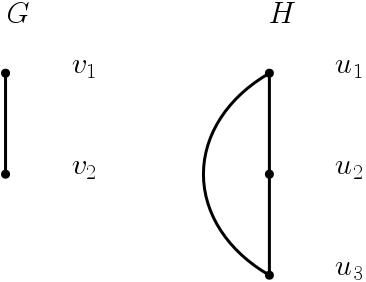
\includegraphics[scale=0.3]{GandH}
	%	\subcaption{}
	\end{minipage}
\begin{minipage}{0.45\textwidth}
	\centering
	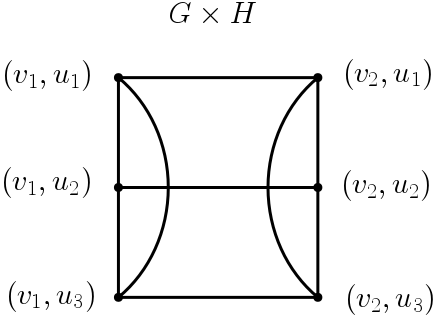
\includegraphics[scale=0.3]{GxH}
%	\subcaption{}
\end{minipage}
\caption{Two graphs and their product graph.}
\end{figure}

\begin{definition}
	\label{def:product_graphs}
	Given two graphs $G=(V(G),E(G))$ and $H=(V(H), E(H))$, the \emph{product graph of $G$ and $H$} is the graph with vertex set $V(G)\times V(H)$ and edge set
	$\{((i_1,j),(i_2,j)):(i_1,i_2)\in E(G), j\in V(H)\}\cup\{((i,j_1),(i,j_2)):(j_1,j_2)\in E(H), i\in V(G)\}$. It is denoted $G\times H$. 
\end{definition} 

In order to investigate the simplex of a product graph, we must better understand its eigenstructure. 

\begin{lemma}
	\label{lem:prod_graph_eigenstructure}
	Let graphs $G$  and $H$ be given. Put $n=|V(G)|$ and $m=|V(H)|$. Suppose $G$ has eigenvalues $\lambda_1\geq \dots\geq \lambda_{n}$ and corresponding eigenvectors $\vp_1,\dots,\vp_{n}$, as usual. Let $H$ have eigenvalues $\mu_1\geq \dots\geq \mu_{m}$ and corresponding eigenvectors $\bpsi_1,\dots,\bpsi_{m}$. Then $G\times H$ has $mn$ eigenvalues $\{\lambda_i+\mu_j\}_{(i,j)i\in[n]\times[m]}$ with eigenvectors $\{f_{i,j}\}_{(i,j)\in[n]\times[m]}$ given by 
	$f_{i,j}(k,\ell) = \vp_i(k)\bpsi_j(\ell)$. 
\end{lemma}

Consequently, with $G$ and $H$ as in Lemma~\ref{lem:prod_graph_eigenstructure}, we see that the product graph yields a simplex $\splx_{G\times H}\in\R^{mn-1}$ with vertices $\{\sv_{ij}\}_{(i,j)\in[n]\times[m]}$ given by 
\[\sv_{ij}(k\ell)=f_{k\ell}(ij)(\lambda_k+\mu_\ell)^{1/2}.\]


\subsection{Examples}
\label{sec:examples}

We now move onto concrete examples of the simplices of particular graphs whose eigenstructures we can compute explicitly. We also compute the graph of perhaps the most well-known simplex:  the probability simplex. 

\paragraph{The complete graph, $K_n$.}
Let us consider the combinatorial simplex $\splx=\splx_{K_n}$.  The Laplacian $\L_{K_n}$ has two eigenvalues: 0 with multiplicity 1 and $n$ with multiplicity $n-1$. To see this, observe that for any $\eig$ perpendicular to $\one$, we have 
\begin{align*}
\L_{K_n}\eig &= \bigg(\vp(1)(n-1)-\sum_{i\neq 1}\eg(i),\dots,\vp(n)(n-1)-\sum_{i\neq n}\eg(i)\bigg) \\
&= \bigg(\vp(1)n - \sum_i \vp(i), \dots,\vp(n)n - \sum_i \vp(i)\bigg) \\
&= (\vp(1)n,\dots,\vp(n)n) = n\eig,
\end{align*}
since $\sum_i\vp(i)=\la \eig,\one\ra =0$. Let $\Q$  described the rotation matrix which rotates each vector  by $\pi/4$  about each axis. Thus $\Q\e_1=\one$, and we can $n-1$ orthogonal eigenvectors $\Q\e_2,\dots,\Q\e_n$. The vertices of $\splx$  are thus given by $\sv_i(j) = \sqrt{n}(\Q\e_{j+1})(i)$. 

\paragraph{The Cycle graph,  $C_n$.}
The cycle graph $C_n$ has edge set $E=\{(i,j):j=i+1\mod n\}$. We assume that $n$ is even for this example. 
We leave it to the reader to verify by direct computation  that the eigenvalues  and eigenvectors of $\L_{C_n}$ are given by 
\[\vp_i(j) = \cos(\frac{2\pi(i-1)j}{n}),\quad \lambda_i = 2-2\cos(\frac{2\pi(i-1)}{n}),\]
for $i=1,\dots,n/2+1$, and 
\[\vp_i(j) = \cos(\frac{2\pi(i-n/2-1)j}{n}),\quad \lambda_i = 2-2\cos(\frac{2\pi(i-n/2-1)}{n}),\]
for $i=n/2+2,\dots,n$. Therefore,  the vertices of $\splx_{C_n}$ are given by  
\begin{equation*}
\sv_i(j) = \begin{cases}
\cos(\frac{2\pi(i-1)j}{n})\bigg(2-\cos(\frac{2\pi(i-\chi(j>n/2+1)n/2 -1)}{n})\bigg),& i\leq n/2+1, \\
\sin(\frac{2\pi(i-n/2-1)j}{n})\bigg(2-\cos(\frac{2\pi(i-\chi(j>n/2+1)n/2 -1)}{n})\bigg),& i> n/2+1.
\end{cases}
\end{equation*}


\paragraph{The probability simplex.} 
Fix  $n\in\N$. The \emph{probability simplex} is the simplex $\widetilde{\splx}_p=\conv(\{\bchi_i\}_{i=1}^n \cup \{\zero\})$. It is most likely the simplex of greatest familiarity to mathematicians and computer scientists, being used to reason geometrically about probability distributions. The probability simplex has centroid $\one/n\neq\zero$ and we will consider its centred version 
\[\splx_p \equiv \widetilde{\splx}_p -  \frac{\J}{n},\]
which has vertices  $\sv_i = \bchi_i - \one/n$, $i<n$, and $\sv_n = -\one/n$. Note that $\sv_j-\sv_n = \bchi_j$ and so 
$\la \bchi_i, \sv_j-\sv_n\ra = \delta_{ij}$. Taking  $\sv_i^\du = \bchi_i$ and $\sv_n^\du = -\sum_i \bchi_i = -\one$ thus gives us the dual vertices. The  angles between the facets of $\splx_p$ are thus defined by 
\begin{equation*}
\cos\theta_{ij}(\splx_p) = - \la \bchi_i,\bchi_j\ra = -\delta_{ij}, 
\end{equation*}
for $i,j\in[n-1]$ and 
\begin{equation*}
\cos\theta_{in}(\splx_p) = \frac{\la \bchi_i,\one\ra}{\norm{1}} = 1/\sqrt{n},
\end{equation*}
for all $i\in[n]$. 
This implies  that $\theta_{ij}(\splx_p) = 0$ for $i\neq j$, $i,j\neq n$ and $\theta_{in}(\splx_p) \in =(0,\pi/2)$. 
Using the  construction of Section~\ref{sec:simplex_to_graph}, we  associate to $\splx_p$ the graph with Laplacian matrix $\Sv(\splx_p^\du)^\to \Sv(\splx_p^\du)$, where $\Sv(\splx_p^\du)=(\sv_1^\du,\dots,\sv_n^\du)$. This matrix has $(i,j)$-th  entry $1$ for $i=j$, 1  for $i=n$ or $j=n$,  and 0 otherwise. This graph thus has each vertex connected  to $n$, but to  no others.  That  is, the graph of the probability simplex $\splx_p$ is  the star graph on  $n$ vertices. 

 



\section{Properties of \texorpdfstring{$\splx_G$}{the Combinatorial Simplex} and \texorpdfstring{$\splx_G^+$}{its inverse}}
\label{sec:S_G}
We now embark on our voyage to understand the mathematical properties of the simplices of a graph. This section is devoted to the study of $\splx_G$ and $\splx_G^+$, while Section \ref{sec:Sn_G} is concerned with $\splxn_G$ and $\splxn_G^+$. For bibliographic purposes, we will encode many of the results as Lemmas even if they are relatively simple. There are many results, and this should enable easier accounting. We begin with three basic properties.

\begin{lemma}
	\label{lem:S_G_basic_properties}
	The following three properties hold: 
	\begin{enumerate}
		\item 	Both $\splx_G$ and $\splx_G^+$ are centred at the origin;
		\item The squared distance between the vertices of $\splx_G^+$ is equal to the effective resistance between the corresponding vertices of $G$; 
		\item For any non-empty $U\subsetneq V$, the faces $\splx_U$ and $\splx^+_{U^c}$ are orthogonal. 
	\end{enumerate}
\end{lemma}
\begin{proof}
	For (i) we  simply compute $\cent(\splx) = n^{-1}\Eval^{-1/2}\Eig^\tp \one =\zero$, since $\la \vp_i,\one\ra =0$ for all $i<n$.  Likewise, $\cent(\splx^+)=\zero$. For (ii), 
	\begin{equation*}
	\norm{\sv_i^+-\sv_j^+}_2^2 = \norm{\sv_i^+}_2^2 + \norm{\sv_j^+}_2^2 - 2\la \sv_i^+,\sv_j^+\ra = \L_G^+(i,i) + \L_G^+(j,j) - 2\L_G^+(i,j) = \effr(i,j).
	\end{equation*}
	The third property follows as a result of the fact that $\splx_G^+$ is dual to $\splx_G$ (Observation \ref{obs:inverse_is_dual}) and Lemma \ref{lem:dual_faces_orthogonal}. 
\end{proof}




Property (ii) in the previous lemma was first noticed by Fielder~\cite[Chapter 6]{fiedler2011matrices}, and was also remarked upon by Van Mieghem \etal~\cite{van2017pseudoinverse} who used it in their study of best spreader nodes in electrical networks. 
We will return to this connection in later sections. We now turn our attention to properties of the angles of a simplex.  

\begin{lemma}
	The combinatorial simplex $\splx_G$ of a graph $G$ is hyperacute iff $\L_G^+$ is a Laplacian.
\end{lemma}
\begin{proof}
	Using Equation~\eqref{eq:cos_theta_ij} and the fact that $\splx_G^+=\splx_G^\du$ (Observation \ref{obs:inverse_is_dual}), we have
	\[\cos \theta_{ij} = -\frac{\la \sv_i^+,\sv_j^+\ra }{\norm{\sv_i^+}_2 \norm{\sv_j^+}_2},\]
	where we recall that $\theta_{ij}$ is the angle between $\splx_\ic$ and $\splx_\jc$. Thus, $\splx_G$ is hyperacute iff
	 \[-\la \sv_i^+,\sv_j^+\ra\\/\norm{\sv_i^+}_2 \norm{\sv_j^+}_2 \in[0,1],\] which occurs iff $\la \sv_i^+,\sv_j^+\ra \leq 0$. In this case $\L_G^+(i,j)\leq 0$, implying that $\L_G^+$ is a Laplacian (recall that it already satisfies the other required properties: $\L_G^+\one=\zero$ and $\L_G^+(i,i)\geq 0$). 
\end{proof}

\begin{corollary}
	\label{cor:Lkn+_laplacian}
	The combinatorial simplex of the complete graph,  $\splx_{K_n}$, is hyperacute. 
\end{corollary}
\begin{proof}
	Let $\L=\L_{K_n}$. 
	It suffices to show by the previous lemma that $\L^+=\L_{K^n}^+$ is a Laplacian. We've already seen that $\L_G^+\one=\zero$ for any $G$, so it remains only to show that $\L^+(k,k)>0$ for all $k\in[n]$ and $\L^+(k,\ell)\leq 0$ for all $k\neq\ell$, i.e., that $\sign(\L(k,\ell))=\sign(\L^+(k,\ell))$ for all $k,\ell$. Recall from Section \ref{sec:examples} that $K_n$ has eigenvalue $n$ with multiplicity $n-1$ and a single zero eigenvalue. Hence, $\L=n\sum_{i<n}\vp_i\vp_i^\tp$ and $\L^+=n^{-1}\sum_{i<n}\vp_i\vp_i^\tp$. 
	Therefore, $\sign(\L(k,\ell)) = \sign(n\sum_{i<n}\vp_i(k)\vp_i(\ell)) = \sign(\sum_{i<n}\vp_i(k)\vp_i(\ell)) = \sign(\L^+(k,\ell))$ which implies the result. 
\end{proof}

Before continuing, we make a brief  detour  to demonstrate how this result combined  with  the link between $\splx_G^+$ and the effective resistance of $G$ allows us to uncover the  total  effective  resistance of certain graphs. Recalling that  $\Rtot_G$  is the  total  effective resistance  in  $G$,  apply Lemma~\ref{lem:S_G_basic_properties} and write  
\begin{align*}
\Rtot_G &= \frac{1}{2}\sum_{i,j\in[n]} \effr(i,j) = \frac{1}{2}\sum_{i,j\in[n]}\norm{\sv_i^+-\sv_j^+}_2^2 \\ 
&= \frac{n}{2}\sum_{in[n]}\norm{\sv_i^+}_2^2 + \frac{n}{2}\sum_{j\in[n]}\norm{\sv_j^+}_2^2 - 2\sum_{i,j\in[n]}\la\sv_i^+,\sv_j^+\ra \\ 
&= n\sum_{i\in[n]}\norm{\sv_i^+}_2^2 - 2\sum_{i\in[n]}\la \L_G(i,\cdot),\one\ra = n\sum_{i\in[n]}\norm{\sv_i^+}_2^2.
\end{align*}

Let $K_n^\alpha$ denote the complete graph on $n$ vertices where each edge has weight $\alpha$. By Corollary~\ref{cor:Lkn+_laplacian}, $\L_{K_n^\alpha}^+=\L_H$ for some graph $H$. Therefore, $\L_{K_n^\alpha}=\L_H^+$ and  $\norm{\sv_i^+(H)}_2^2 = \norm{\sv_i(\L_{K_n^\alpha})}_2^2$.  If $K_n$ is the unweighted complete graph, we see that $\L_{K_n^\alpha}=\alpha\L_{K_n}$. Using  that $L_{K_n}$ has eigenvalue $n$ with multiplicity $n-1$  (Section~\ref{sec:examples}) gives $L_{K_n^\alpha}=\alpha n\sum_{i<n}\vp_i\vp_i^\tp$, meaning that $\L_{K_n^\alpha}=\L_H^+$ has eigenvalue $\alpha n$ with multiplicity $n-1$. The effective resistance of $H$ is then 
\begin{equation*}
\Rtot_H = n\Tr(\L_H^+) = \alpha(n-1). 
\end{equation*}
Moreover, $\L_H$ has eigenvalue $(\alpha n)^{-1}$ with multiplicity $n-1$, and  is therefore a complete graph with weights $(\alpha n^2)^{-1}$. We have proven the  following:  

\begin{lemma}
	For any complete graph $H$ on $n$ vertices with uniform edge weights  $(\alpha n^2)^{-1}$ for any $\alpha$,  $\Rtot_H = \alpha (n-1)$. 
\end{lemma}



As Fiedler pointed out~\cite{fiedler1993geometric}, the correspondence also allows us to answer questions related to the distribution of angles of simplices. It is not, for example, a priori obvious that all distributions of angles  are possible in a hyperacute simplex, in the following sense. 

\begin{lemma}
	For every $n-1\leq k \leq \binom{n}{2}$, there exists a hyperacute simplex on $n$ vertices with $k$ strictly acute interior angles. 
\end{lemma}
\begin{proof}
	Fix $k$ and consider a connected graph on $n$ vertices with $k$ edges (note the importance that $k\geq n-1$). The interior angles $\{\theta_{ij}^+\}_{i,j}$ of $\splx_G^+$ obey $\cos\theta_{ij} = w(i,j) / \sqrt{w(i)w(j)}$, hence $\theta_{ij}=\pi/2$ whenever $w(i,j)=0$, and $\theta_{ij}\in(0,\pi/2)$ for all $(i,j)\in E(G)$. Therefore, $\splx_G^+$ meets the desired criteria. 
\end{proof}



The following lemma presents an alternate characterization of the simplex, and was first proved by Devriendt  and Van Mieghem~\cite{devriendt2018simplex}. As they notice, the following representation provides an easy way to check whether a given point lies inside the simplex. As our proof is similar  to theirs, we move  it to  Appendix~\ref{sec:app_proofs_correspondence}. 

\begin{lemma}[\cite{devriendt2018simplex}]
\label{lem:S_alt_desc}
For a simplex $\splx$ of a graph $G$, 
\begin{equation}
\label{eq:S_alt_desc}
    \splx=\bigg\{\x\in \R^{n-1}:\x^\tp\Sv^++\frac{\one^\tp}{n}\geq \zero^\tp\bigg\}.
\end{equation}
\end{lemma}

Just as each facet of a tetrahedron is contained in a plane and each edge is contained in an infinite line, each face $\splx_U$ of a simplex $U$ is contained in a \emph{flat} (i.e., a linear subspace shifted by some constant\footnote{Also  called an affine subspace.}) of dimension $|U|-1$. The following lemma helps characterize these flats. 

\begin{lemma}
\label{lem:SUsubset}
Let $\splx$ be the simplex of a graph $G=(V,E,w)$, and fix $U\subset V$. For any non-empty $E\subset U^c$,
\begin{equation*}
    \splx_U \subset \bigg\{\x\in\R^{n-1}: \sum_{i\in E}\la \x,\sv_i^+\ra +\frac{|E|}{n}=  0\bigg\},
\end{equation*}
and
\begin{equation*}
    \splx^+_U \subset \bigg\{\x\in\R^{n-1}: \sum_{i\in E}\la \x,\sv_i\ra +\frac{|E|}{n}=  0\bigg\},
\end{equation*}
\end{lemma}
\begin{proof}
Let $\x\in\splx_U$ be arbitrary. For any $i\in U^c$ we have $\la \x,\sv_i^+\ra = -1/n$. Hence, for any $E\subset U^c$
\[\sum_{i\in E}\la \x,\sv_i^+\ra + \frac{|E|}{n} = \sum_{i\in E}\bigg(\la \x,\sv_i^+\ra+\frac{1}{n}\bigg)=\sum_{i\in E}\bigg(\frac{1}{n}-\frac{1}{n}\bigg)=0,\]
implying that $\x$ is in the desired set. 
\end{proof}

Lemma \ref{lem:SUsubset} gives us an alternate way to prove Lemma \ref{lem:S_alt_desc}. For any $i$,  taking $U=N\setminus \{i\}$ and $E=\{i\}$, it implies that $\splx_{\{i\}^c}$ is a subset of the hyperplane 
\begin{equation}
\label{eq:Hi}
 \H_i\equiv \{\x\in\R^{n-1}:\la \x,\sv_i^+\ra+1/n=0\}.
\end{equation}
All points in the simplex $\splx$ lie to one side of $\splx_{\{i\}^c}$, i.e., they lie in the halfspace 
\[\H_i^{\geq } \equiv \{\x\in\R^{n-1}:\la \x,\sv_i^+\ra+1/n\geq0\}.\]
(We know it is this halfspace because $\zero\in\splx\cap\H_i^{\geq }$.) The simplex is the interior of the region defined by the intersection of the faces $\splx_{\{i\}^c}$, i.e.,   
\begin{equation}
\label{eq:splx_bigcapH_i}
    \splx=\bigcap_i \H_i^{\geq }.
\end{equation}
Moreover, $\x\in \bigcap_i\H_i^{\geq }$ iff $\la \x,\sv_i^+\ra +1/n\geq 0$ for all $i$, i.e., $(\la \x,\sv_1^+\ra,\dots,\la \x,\sv_n^+\ra) + \one/n\geq \zero$, meaning $\x$ satisfies \eqref{eq:S_alt_desc}.  We emphasize that a very similar discussion applies to $\splx^+$, in which case one has 
\begin{equation}
\label{eq:splx^+_bigcapH_i}
\splx^+=\bigcap_i (\H_i^+)^{\geq },
\end{equation}
for $(\H_i^+)^{\geq } \equiv \{\x\in\R^{n-1}:\la \x,\sv_i\ra + 1/n\geq 0\}$. 

\begin{figure}
	\centering
	\includegraphics[scale=0.5]{HI_plane}
	\caption{An illustration of the combinatorial simplex $\splx_G\subset\R^3$ and its face $\splx_\ic$ contained in the hyperplane $\H_i$. }
	\label{fig:Hi_plane}
\end{figure}


\paragraph{Centroids and altitudes.} 
We now turn to investigating the centroids and altitudes of the simplices, and how they relate to properties of the underlying graph. We begin by exploring the relationships between properties of the simplices themselves. 

Recall that the altitude between $\splx[U]$ and $\splx[U^c]$ of a simplex $\splx$ is denoted $\alt(\splx_U)$ and is the unique vector $\p-\q$ where  $\p\in \splx_{U^c}$ and $\q\in\splx_{U}$ which lies in the orthogonal complement of both $\splx_U$ and $\splx_{U^c}$. One would thus expect that $\alt(\splx_U)$ and $\alt(\splx_{U^c})$ to be antiparallel; a fact verified by Lemma \ref{lem:complimentary_centroids}.  

In what follows,  we will often write $\cent_U$ for $\cent(\splx_U)$ (resp., $\cent_U^+$ for $\cent(\splx_U^+)$) and $\alt_U$ for $\alt(\splx_U)$ (resp., $\alt_U^+$ for $\alt(\splx_U^+)$). 

\begin{lemma}[\cite{devriendt2018simplex}]
\label{lem:complimentary_centroids}
Let $U\subset V$ be non-empty. Then the vectors $\cent(\splx_U)$ and $\cent(\splx_{U^c})$ are antiparallel. In particular, $(n-|U|)\cent(\splx_{U^c}) = |U|\cent(\splx_{U})$ and 
\[\frac{\cent(\splx_U)}{\norm{\cent(\splx_U)}_2}=-\frac{\cent(\splx_{U^c})}{\norm{\cent(\splx_{U^c})}_2}.\]
\end{lemma}
\begin{proof}
This is a straightforward computation: Observing that $\bchi_U=\one-\bchi_{U^c}$ we have  
\[\cent_U = |U|^{-1}\Sv\bchi_U = |U|^{-1}\Sv(\one-\bchi_{U^c})=-|U|^{-1}\Sv\bchi_{U^c}=-|U|^{-1}\frac{|U^c|}{|U^c|}\Sv\bchi_{U^c}=\frac{n-|U|}{|U|}\cent_{U^c},\]
where we've used that $\Sv\one=\zero$. This proves the first result; the second follows from normalizing the two vectors.
\end{proof}

We would now like to examine the relationships between altitudes and centroids in the simplex and its inverse. We will demonstrate that centroids of opposing faces are antiparallel, and that the centroid of the face $U$ is parallel to the altitude of originating from the face generated by $U$ in its inverse. First however, we require the following technical result. 

\begin{lemma}
	\label{lem:S_U_ortho_complement}
	Any vector perpendicular to $\splx_U$ can be written as $\Sv^+(\f_{U^c}+\alpha \bchi_U)$ for some $\alpha\in\R$ and vector $\f_{U^c}$ such that $\f_{U^c}(U)=\zero$. 
\end{lemma}
\begin{proof}
	Let $\y\in\R^{n-1}$ be orthogonal to $\splx_U$. Since $\rank(\Sv^+)=n-1$, we can find some $\z$ such that $\y=\Sv^+\z=\sum_{i\in U^c}\sv_i^+z(i) + \sum_{j\in U}\sv_j^+z(j)$. Define $\f$ by $\f(U^c)=\z(U^c)$ and $\f(U)=\zero$ and $\z_{U^c}$.  We can then write $\y$ as $\Sv^+\f+\sum_{j\in U}\sv_j^+z(j)$, so we must show that $\z(U)$ is a constant vector. The orthogonality of $\y$ to $\splx_U$ implies that for every two barycentric coordinates $\x_U$ and $\y_U$ with $\x(U^c)=\y(U^c)=\zero$, 
	\begin{align}
	0 &= \la \y,\Sv\x_U-\Sv\y_u\ra \notag \\
	&= \sum_{i\in U^c}z(i) \la \sv_i^+,\Sv(\x_U-\y_U)\ra + \sum_{j\in U}z(j)\la \sv_j^+,\Sv(\x_U-\y_U)\ra  \notag \\
	&= \sum_{j\in U}z(j)\la \sv_j^+,\Sv(\x_U-\y_U)\ra, \label{eq:lem_ortho_complement1}
	\end{align} 
	where the final inequality follows because $\sv_i^+$ is orthogonal to $\splx_U$ for $i\in U^c$ by Lemma \ref{lem:S_G_basic_properties}.
	 Now, for $j\in U$, 
	\begin{align}
	\la \sv_j^+,\Sv(\x_U-\y_U)\ra &= \bchi_j^\tp \Sv^+\Sv(\x_U-\y_U) = \bchi_j^\tp \bigg(\I - \frac{\J}{n}\bigg)(\x_U-\y_U) = \bchi_j^\tp (\x_U-\y_U). \label{eq:lem_ortho_complement2}
	\end{align}
	Suppose for contradiction that $z(k)\neq z(j)$ for some $k,j\in U$. Put $\x_U = \bchi_k$ and $\y_U=\bchi_j$. Using Equation  \eqref{eq:lem_ortho_complement2} write \eqref{eq:lem_ortho_complement1} as 
	\begin{align*}
	z(k)\bchi_k^\tp(\bchi_k-\bchi_j) + z(j)\bchi_j^\tp(\bchi_k -\bchi_j) + \sum_{\ell\in U^c,\ell\neq j,k}z(\ell)\bchi_\ell^\tp(\bchi_k-\bchi_j) = z(k)-z(j)\neq 0,
	\end{align*}
	a contradiction. 
\end{proof}

We can now proceed to the main result. 

\begin{lemma}
\label{lem:alt_and_centroid}
For a simplex $\splx$ of a graph $G=(V,E)$ and any $U\subset V$, $U\neq\emptyset$, 
\begin{equation}
\label{eq:alt_and_centroid}
    \frac{\alt(\splx_U)}{\norm{\alt(\splx_{U})}_2}=\frac{\cent^+(\splx_{U^c})}{\norm{\cent^+(\splx_{U^c})}_2}=-\frac{\cent^+(\splx_{U})}{\norm{\cent^+(\splx_{U})}_2},
\end{equation}
and 
\begin{equation*}
    \frac{\alt^+(\splx_U)}{\norm{\alt^+(\splx_{U})}_2}=\frac{\cent(\splx_{U^c})}{\norm{\cent(\splx_{U^c})}_2}=-\frac{\cent(\splx_{U})}{\norm{\cent(\splx_{U})}_2}.
\end{equation*}
\end{lemma}
\begin{proof}
We prove the first set of equalities only; the second is obtained similarly. By definition, $\alt_U$ is orthogonal to both $\splx_U$ and $\splx_{U^c}$. Lemma \ref{lem:S_U_ortho_complement} then implies both that 
\begin{equation*}
\alt_U = \Sv^+\f + \alpha \Sv^+\bchi_U,
\end{equation*}
and 
\begin{equation*}
\alt_U = \Sv^+\g + \beta\Sv^+\bchi_{U^c},
\end{equation*}
for some $\alpha,\beta\in\R$, and vectors $\f,\g$ with $\f(U)=\zero$ and $\g(U^c)=\zero$. In particular then, 
\begin{equation}
\label{eq:lem_alt_centroid1}
\frac{\Sv^+(\f+\alpha\bchi_U)}{\norm{\Sv^+(\f+\alpha\bchi_U)}_2}=\frac{\Sv^+(\g+\beta\bchi_{U^c})}{\norm{\Sv^+(\g+\beta\bchi_{U^c})}_2}.
\end{equation}
By Lemma \ref{lem:complimentary_centroids}, taking $\f=\pm\bchi_{U^c}/|U^c|$, $\g=\mp\bchi_U/|U|$, and $\alpha=\beta=0$ yield solutions to the above equation. We have thus obtained Equation \eqref{eq:alt_and_centroid} up to its sign; 
it remains to determine whether $\alt(\splx_U)$ is parallel to antiparallel to $\cent(\splx_U)$. Since it is one of the two, we have 
\[\frac{\la \alt_U,\cent^+_U\ra}{\norm{\alt_U}_2\norm{\cent^+U}_2}\in\{1,-1\},\]
hence to see that they are antiparallel it suffices to show that $\la \alt_U,\cent^+U\ra<0$. Let $\alt_U= \Sv\y_{U^c}-\Sv\z_U$ for barycentric coordinates $\y_{U^c}$ and $\z_U$ representing the faces $\splx_{U^c}$ and $\splx_U$. Then, 
\begin{align*}
\la \alt_U,\cent^+_U\ra &= \frac{1}{n}\la \Sv(\y_{U^c}-\z_U),\Sv\bchi^+_U\ra \\
&= \frac{1}{n}(\y_{U^c}^\tp-\z_U^\tp)\bigg(\I-\frac{\J}{n}\bigg)\bchi_U\\ &=-\frac{1}{n}\z_U^\tp\bchi_U  - \frac{1}{n^2}(\y_{U^c}^\tp-\z_U^\tp)\one\one^\tp\bchi_U\\
&= -\frac{1}{n}<0.
\end{align*}
Therefore, $\alt_U$ is indeed antiparallel to $\cent^+_U$, meaning that the correct signage is $\f=\bchi_{U^c}/|U^c|$ and $\g=-\bchi_U/|U|$. Thus, 
\begin{equation*}
\frac{\alt_U}{\norm{\alt_U}_2}=\frac{\Sv^+\bchi_{U^c}}{\norm{ \Sv^+\bchi_{U^c}}_2}=-\frac{\Sv^+\bchi_{U}}{\norm{\Sv^+\bchi_U}_2},
\end{equation*}
which is Equation \eqref{eq:alt_and_centroid}. 
\end{proof}

\begin{remark}
	We note that there are no other solutions, up to scaling, of the system of equations for $\alt_U$ in the previous proof. Indeed, let $\f,\g,\alpha,\beta$ satisfy the equations. 
	Then 
	\[\Sv^+(\f-\beta\bchi_{U^c}) + \Sv^+(\alpha\bchi_U-\g)=\zero, \]
	so $f-\beta\bchi_{U^c} + \alpha\bchi -g\in \ker(\Sv^+) = \spn(\one)$, implying that $\f-\beta\bchi_{U^c} = k\bchi_{U^c}$ and $\alpha\bchi_U -g=k\bchi_{U}$ for some $k\in \R$, which yields the same solution as in the proof. 
\end{remark}

Whereas the previous few lemmas explored relationships among $\splx_G$ and $\splx_G^+$ only, we now begin to observe several connections between the geometry of the simplices and properties of the graph. We begin by recalling that given $U\subset V(G)$ the \emph{cut-set} of $U$ is 
\[\partial U \equiv (U\times U^c)\cap E(G)= \{(i,j)\in E(G): i\in U, j\in U^c\}.\]
Noting that $|\bchi_U(i)-\bchi_U(j)|=\chi_{(i,j)\in \partial U}$, we see that
\begin{align*}
w(\partial U) = \sum_{i,j\in E} w(i,j)|\bchi_U(i)-\bchi_U(j)| = \sum_{i,j\in E} w(i,j)(\bchi_U(i)-\bchi_U(j))^2 = \Lf(\bchi_U). 
\end{align*}
Moreover, $\norm{\cent(\splx_U)}^2_2 = \la |U|^{-1} \Sv\bchi_U,|U|^{-1} \Sv\bchi_U\ra = |U|^{-2} \Lf(\bchi_U)$ and so 
\begin{equation}
\label{eq:c(S_U)}
\norm{\cent(\splx_U)}_2^2 = \frac{w(\partial U)}{|U|^2}.
\end{equation}
Via the same process we can also obtain an equivalent expression for the centroid of the inverse simplex: 
\begin{equation}
\label{eq:c(S+_U)}
\norm{\cent(\splx^+_U)}_2^2 = \frac{w(\partial^+ U)}{|U|^2},
\end{equation}
where we follow the notation of \cite{devriendt2018simplex} and define \begin{equation}
\label{eq:w(d^+)}
w(\partial^+U) \equiv  \la \Sv^+\bchi_U,\Sv^+\bchi_U\ra=\la \bchi_U,\L^+\bchi_U\ra=\Lf^+(\bchi_U).
\end{equation} 
Equations \eqref{eq:c(S_U)} and \eqref{eq:c(S+_U)} were also given in \cite{devriendt2018simplex}. As a sanity check, we note that the equations are consistent with the facts that $\norm{\sv_i}_2^2 = w(i)$ and $\norm{\sv_i^+}_2^2 = \L^+(i,i) = \Lnf^+(\bchi_i)$. These equations allow us to give an interesting correspondence between the sizes of the altitudes and cut-sets of $G$. 

\begin{lemma}
\label{lem:||alt||}
For any non-empty $U\subset V$, $\norm{\alt^+_U}_2^2=1/w(\partial U)$ and $\norm{\alt_U}_2^2 = 1/w(\partial^+ U)$.  
\end{lemma}
\begin{proof}
By definition of the altitude there exists barycentric coordinates $\x_U$ and $\x_{U^c}$ such that $\alt^+_U = \Sv^+(\x_U-\x_{U^c})$. Combining this representation of $\alt^+_U$ with that given by Lemma \ref{lem:alt_and_centroid}, write 
\begin{align*}
    \norm{a^+_U}_2 = \frac{\la a^+_U,a^+_U\ra }{\norm{a^+_U}_2} = \frac{\la \Sv^+(\x_{U^c}-\x_{U}), c_{U^c}\ra }{\norm{c_{U^c}}_2} = \frac{\la \Sv^+(\x_{U^c}-\x_{U}), \Sv\bchi_{U^c}\ra }{\sqrt{w(\partial U^c)}},
\end{align*}
where the final equality comes from using the definition of the centroid in the numerator, and Equation~\eqref{eq:c(S_U)} in the denominator. Recalling the relation between $\Sv$ and $\Sv^+$ given by Equation~\eqref{eq:sv+sv} and that $\x_U$ and $\x_{U^c}$ are barycentric coordinates, we can rewrite the above as 
\[\frac{(\x_{U^c}-\x_{U})^\tp(\I-\one\one^\tp/n)\bchi_{U^c}}{\sqrt{w(\partial U^c)}}=\frac{1}{\sqrt{w(\partial U^c)}}. \]
Squaring both sides while noting that $\partial U = \partial U^c$ completes the proof of the first equality. For the second, we proceed in precisely the same manner to obtain $\norm{a_U}_2^2 = 1/w(\partial^+ U^c)$. However, it's not immediately obvious that $w(\partial^+U^c)=w(\partial^+U)$. To see this, first recall that $\Sv^+\one = \Eval^{-1/2}\Eig^\tp\one = \zero$, and so 
\begin{align*}
w(\partial^+ U^c) &= \la \Sv^+\bchi_{U^c},\Sv^+\bchi_{U^c}\ra  \\
&= \la \Sv^+(\one - \bchi_{U}),\Sv^+(\one - \bchi_{U})\ra  \\
&= \la \Sv^+\bchi_{U},\Sv^+\bchi_{U}\ra = w(\partial^+ U).
\qedhere
\end{align*}
\end{proof}

The aforementioned astute reader may have noticed that the above result implies something about the computational difficulty of determining the length of the minimum and maximum altitudes in hyperacute simplices. We tell this reader to ``hold their horses''---this result and others like it will be presented in Chapter \ref{chap:algorithmics}. 

The next two lemmas were both proven by Devriendt and Van Mieghem~\cite{devriendt2018simplex}, extending work done by Fiedler. 
The following lemma gives an explicit expression for the altitudes in terms of graph properties and the inverse centroid. 

\begin{lemma}
\label{lem:alt}
For any non-empty $U\subset V$, 
\[\alt_U=\frac{n-|U|}{w(\partial^+ U)}\cent^+_{U^c},\quad \text{and}\quad \alt^+_U = \frac{n-|U|}{w(\partial U)} \cent_{U^c}.\]
\end{lemma}
\begin{proof}
This is a consequence of identities \eqref{eq:c(S_U)} and \eqref{eq:c(S+_U)} and Lemmas \ref{lem:alt_and_centroid} and \ref{lem:||alt||}. Applying the latter and then the former, observe that 
	\[\alt_U = \frac{\norm{\alt_U}_2}{\norm{\cent^+_{U^c}}_2}\cent^+_{U^c} =
\bigg(\frac{1}{\sqrt{w(\partial^+ U^c)}} \bigg/\frac{\sqrt{w(\partial^+U)}}{|U^c|} \bigg)\cent^+_{U^c} = \frac{n-|U|}{w(\partial^+U)}c^+_{U^c},\]
where we've once against used that $w(\partial^+ U^c )=w(\partial^+ U)$. A similar computation holds for $\alt_U^+$.  
\end{proof}

Just as one generalizes the incidence of a vertex to the neighbourhood of a set of vertices, one can generalize an edge to the incidence between groups of vertices, as
\[\partial U_1\cap \partial U_2 = \{(i,j)\in E(G), i\in U_1,j\in U_2\},\]
for $U_1,U_2\subset V(G)$. The final lemma gives an expression for the weight (or size) of this set in terms of the altitudes and centroids of the simplices. 


\begin{lemma}
	\label{lem:alt_centroid_dot_product}
Let $U_1,U_2\subset V$ with $U_1\cap U_2=\emptyset$. Then 
\begin{equation*}
    \la \cent(\splx_{U_1}),\cent(\splx_{U_2})\ra = - \frac{w(\partial U_1\cap \partial U_2)}{|U_1||U_2|},\quad\text{and}\quad \la \alt^+_{U_1},\alt^+_{U_2}\ra = -\frac{w(\partial U_1^c\cap \partial U_2^c)}{w(\partial U_1)w(\partial U_2)}.
\end{equation*}
\end{lemma}
\begin{proof}
For $i,j\in V$, $i\sim j$, observe that 
\[\bchi_{U_1}^\tp \L_{i,j}\bchi_{U_2}=
\begin{cases}
-w(i,j),& i\in U_1,j\in U_2\text{ or }i\in U_2,j\in U_1,\\
0,&\text{otherwise.}
\end{cases}\]
Therefore, 
\begin{align*}
    \la \cent_{U_1},\cent_{U_2}\ra &= \la |U_1|^{-1}\Sv\bchi_{U_1},|U_2|^{-1}\Sv\bchi_{U_2}\ra = |U_1|^{-1}|U_2|^{-1} \bchi_{U_1}^\tp \L_G\bchi_{U_2} \\
    &= |U_1|^{-1}|U_2|^{-1}\sum_{i\sim j} \bchi_{U_1}^\tp \L_{(i,j)}\bchi_{U_2} = |U_1|^{-1}|U_2|^{-1}\sum_{(i,j)\in \partial U_1\cap \partial U_2} -w(i,j),
\end{align*}
which proves the first equality. The second is shown similarly by employing Lemma \ref{lem:alt} and the previous identity:
\begin{align*}
    \la \alt^+_{U_1},\alt^+_{U_2}\ra &= \frac{|U_1^c||U_2^c|}{w(\partial U_1) w(\partial U_2)}\la \cent_{U_1^c},\cent_{U_2^c}\ra
    =-\frac{w(\partial U_1^c\cap \partial U_2^c)}{w(\partial U_1)w(\partial U_2)}.\qedhere
\end{align*}
\end{proof}

Given the number of---often related and interacting---results in this section, it may be worth providing a brief summary. The important takeaways are that (i) the geometry of the inverse simplex $\splx^+$ is intimately related to the effective resistance of the graph (Lemma \ref{lem:S_G_basic_properties}) and (ii) the lengths of the altitudes and centroids of $\splx$ and $\splx^+$ are proportional to the weights of cuts (Equations \eqref{eq:c(S_U)}, \eqref{eq:c(S+_U)}, Lemmas \ref{lem:||alt||}, \ref{lem:alt}, \ref{lem:alt_centroid_dot_product}). 

\section{Properties of \texorpdfstring{$\splxn_G$}{the normalized Simplex} and \texorpdfstring{$\splxn_G^+$}{and its inverse}}
\label{sec:Sn_G}

Here we study the normalized simplex $\splxn_G$ of the connected graph $G=(V,E,w)$---which we again fix throughout this section---a somewhat less accessible object than its unnormalized counterpart.  The normalized simplex is, roughly speaking, distorted by the weights of the vertices. Consequently, many of the relationships between $\splx_G$ and $\splx_G^+$ are lost between $\splxn_G$ and $\splxn_G^+$. The first issue is that, in general, $\splxn_G$ and its inverse are not centred at the origin. Indeed, recall that the zero eigenvector $\vpn_n$ of $\Ln_G$ sits in the space $\spn(\W^{1/2}_G\one)$, which is distinct from $\spn(\one)$ unless $\W^{1/2}_G=d\I$ for some $d$, in which case $G$ is regular.
If $G$ is not regular, we thus have that $\vp_i \in \spn(\W^{1/2}_G\one)\subset \spn(\one)^\perp$ for all $i<n$ implying that $\la \vp_i,\one\ra \neq 0$. In this case then,  
 \[\cent(\splxn_G) = \frac{1}{n} \Evaln^{1/2}\Eign^\tp \one = \frac{1}{n} \begin{pmatrix}
 \sqrt{\lambda_1}\la \vp_1,\one\ra \\
 \vdots \\
\sqrt{ \lambda_{n-1}}\la \vp_{n-1},\one \ra
 \end{pmatrix}\neq \zero.\]
The above argument proves the following.

\begin{lemma}
	\label{lem:centroid_normalized}
	The centroid of $\splxn_G$ coincides with the origin of $\R^{n-1}$ iff $G$ is regular. 
\end{lemma}

Given this, one might wonder whether the origin is even a point in the simplex $\splxn$. It is easily seen that it is, however. Consider the barycentric coordinate $\u = \sqrt{\w}/\norm{\sqrt{\w}}_1$, where $\sqrt{\w}=(w(1)^{1/2}, \dots, w(n)^{1/2})$. Since all eigenvectors $\vpn_i$, $i<n$ are orthogonal to $\vp_n \in\spn(\w^{1/2})$ it follows that $\zero = \Svn\u\in\splxn$. 

The next set of properties which don't hold between $\splxn$ and $\splxn^+$ are the orthogonality relationships present between a simplex and its dual. That is, in general $\splxn^+_G$ is the not the dual of $\splxn_G$. 

\begin{lemma}
	\label{lem:inverse_not_dual}
	The inverse simplex $\splxn_G^+$ is the dual of $\splxn_G$ iff $G$ is regular. 
\end{lemma}
\begin{proof}
	For any $i,j,k\in\N$ write 
	\begin{equation}
	\label{eq:lem_inverse_not_dual}
	\la \svn_i^+,\svn_j-\svn_k\ra = \delta_{ij} - \delta_{ik} + \frac{\sqrt{w(i)w(k)}}{n} - \frac{\sqrt{w(i)w(j)}}{n}.
	\end{equation}
	First suppose that $G$ is regular; so  $w(r)=w(s)$ for all $r,s$. Then for $i\neq k$, Equation \eqref{eq:lem_inverse_not_dual} becomes $\la \svn_i^+,\svn_j-\svn_k\ra = \delta_{ij}$. Since $k$ was arbitrary, we see that $\{\svn_i^+\}$ is the sister pair of $\{\svn_j-\svn_k\}$. Conversely, suppose $G$ is not regular and let $i,k$ obey $0\neq w(i)\neq w(k)$. Taking $i=j\neq k$ in \eqref{eq:lem_inverse_not_dual} we see 
	\[\la \svn_i^+,\svn_i-\svn_k\ra = 1 - \frac{\sqrt{w(i)}}{n}(\sqrt{w(k)}-\sqrt{w(i)})\neq 1,\]
	so $\{\svn_i^+\}$ is not the sister set of $\{\svn_j-\svn_k\}$, completing the argument. 
\end{proof}

A consequence of the previous Lemma is that we can no longer apply Lemma \ref{lem:dual_faces_orthogonal} (regarding the orthogonality of $\ssplx_U$ and $\ssplx_{U^c}^\du$) to obtain information concerning $\splxn_U$ and $\splxn_{U^c}^+$. The following two lemmas and corresponding corollary address the link between these faces, and---rather unfortunately---demonstrate that indeed, they are not orthogonal in general. 
The first gives sufficient conditions under which the faces are orthogonal, the second provides necessary conditions. 
Before we state the lemmas, recall from Section \ref{sec:background_spectral} that a subset of vertices is weight  (or degree) homogenous if each vertex in the set has the same weight. 

\begin{lemma}
	\label{lem:Sn_perp_homogenous}
	Let $U_1,U_2\subset V(G)$ be two non-empty, weight homogenous subsets such that $U_1\cap U_2=\emptyset$. Then the faces $\splxn^+[U_1]$ and $\splxn[U_2]$ are orthogonal. 
\end{lemma}
\begin{proof}
	Suppose $w(i)=w_1$ for all $i\in U_1$ and $w(i)=w_2$ for all $i\in U_2$. Let $\x_{U_1}$ be the barycentric coordinate of any point in $\splxn^+[U_1]$ and $\x_{U_2}$ that of any point in $\splxn[U_2]$. 
	\begin{align*}
	\la \Svn^+\x_{U_1},\Svn\x_{U_2}\ra &= \x_{U_1}^\tp \bigg(\I-\frac{\sqrt{\w}\sqrt{\w}^\tp}{\vol(G)}\bigg) \x_{U_2}\\
	&= \x_{U_1}^\tp\x_{U_2} - \frac{1}{\vol(G)}\sum_{i\in U_1}\x_{U_1}(i)\sqrt{w(i)}\sum_{j\in U_2}\x_{U_2}(j) \sqrt{w(j)} \\
	&= -\frac{1}{\vol(G)}\sqrt{w_1w_2}\sum_{i\in U_1}\x_{U_1}(i) \sum_{j\in U_2}\x_{U_2}(j) = -\frac{\sqrt{w_1w_2}}{\vol(G)},
	\end{align*} 
	where the second equality is due to fact that $U_1\cap U_2=\emptyset$. This demonstrates that $\la \Svn^+\x_{U_1},\p-\q\ra=0$ for any $\p,\q\in\splxn[U_2]$, completing the proof. 
\end{proof}

\begin{lemma}
	\label{lem:Sn_not_homogeneous}
	Suppose  $U_1\subset V(G)$ is not degree homogeneous. Then for all $U_2\subset V(G)$ then faces $\splxn[U_1]$ (resp., $\splxn^+[U_1]$) and $\splxn^+[U_2]$ (resp., $\splxn[U_2]$) are not orthogonal. 
\end{lemma}
\begin{proof}
	We show that $\splxn[U_1]$ and $\splxn^+[U_2]$ are not orthogonal; the other case is nearly identical. Let $i,j\in U_1$ be such that $w(i)\neq w(j)$ and consider the points $\p=\Svn\bchi_i,\q=\Svn\bchi_j\in\splxn[U_1]$. For any $\Svn^+\x\in\splxn^+[U_2]$, performing the usual arithmetic yields
	\begin{align*}
	\la \Svn^+\x,\p-\q\ra &= \frac{1}{\vol(G)} \sum_{k\in U_2}\sqrt{w(k)}x(k)(\sqrt{w(j)}-\sqrt{w(j)}) \neq 0.\qedhere
	\end{align*}
\end{proof}

We state a consequence of Lemmas \ref{lem:Sn_perp_homogenous} and \ref{lem:Sn_not_homogeneous} which exemplifies a clear contrast between  the combinatorial simplices and the normalized simplices.   

\begin{corollary}
	\label{cor:Sn_orthog_iff_regular}
	The vertex $\svn_i^+$ (resp., $\svn_i$) is orthogonal to $\splxn_\ic$ (resp., $\splxn^+_\ic$) iff $G[\ic]=G[V\setminus\{i\}]$ is regular. 
\end{corollary}
\begin{proof}
	If $G[\ic]$ is regular then $\ic$ is weight homogenous. By Lemma~\ref{lem:Sn_perp_homogenous} $\splxn[\{i\}]=\svn_i$ (resp., $\splxn^+[\{i\}]=\svn_i^+$) is orthogonal to $\splxn[\ic]$ (resp., $\splxn^+[\ic]$). (Note that the singleton $\{i\}$ is clearly degree homogeneous.) Conversely, if $G[\ic]$ is not regular then by Lemma~\ref{lem:Sn_not_homogeneous} $\svn_i$ (resp., $\svn_i^+$) is not orthogonal to $\splxn[\ic]$ (resp., $\splxn^+[\ic]$).
\end{proof}

\paragraph{Centroids and altitudes.}
Let us attempt to parallel the arguments given in Section~\ref{sec:S_G}  concerning the centroids and altitudes of $\splx_G$ and $\splx_G^+$. For the normalized Laplacian we have
\begin{align}
\Lnf(\bchi_U)&=\sum_{i\sim j}w(i,j) \bigg(\frac{\bchi_U(i)}{\sqrt{w(i)}}-\frac{\bchi_U(j)}{\sqrt{w(j)}}\bigg)^2 \notag \\
&= \sum_{i\in U,j\in U^c}w(i,j)\bigg(\frac{\bchi_U(i)}{\sqrt{w(i)}}-\frac{\bchi_U(j)}{\sqrt{w(j)}}\bigg)^2 \notag \\
&= \sum_{i\in U,j\in U^c}w(i,j)\frac{\bchi_U(i)}{w(i)} \notag \\
&= \sum_{i\in U}\frac{1}{w(i)} \sum_{j\in \partial(i)\cap U^c}w(i,j) \notag \\
&= \sum_{i\in U}\frac{w_{G[i+U^c]}(i)}{w(i)}, \label{eq:Lnf(chiU)}
\end{align}
where we've used the shorthand $i+U^c = \{i\}\cup U^c$ and we recall that $G[I]$ is the graph restricted to the vertices in $I$. 
To interpret the above quantity, we might define  
\[\gamma(i,B)\equiv \frac{w_{G[i+B^c]}(i)}{w(i)},\]
as the \emph{fractional weight of $i$ in $B$}. 
Further defining $\gamma(A,B)$ as the \emph{total fractional weight from $A$ to $B$}:
\[\gamma(A,B) \equiv \sum_{i\in A}\gamma(i,B), \]
we have 
$\Lnf(\bchi_U) = \gamma(U,U^c)$, 
and so the length of the centroid $c(\splxn_U)$ captures the total fraction of weight between $U$ and $U^c$:
\begin{equation}
\label{eq:c(SnU)}
\norm{c(\splxn_U)}_2^2 = \frac{1}{|U|^2}\la \Svn\chi_U,\Svn\chi_U\ra = \frac{1}{|U|^2}\Lnf(\chi_U) = \frac{1}{|U|^2} \gamma(U,U^c),
\end{equation}
which is the equivalent to Equation \ref{eq:c(S_U)} for the normalized simplex. Performing a similar computation for $\cent(\splxn^+_U)$ doesn't seem to yield anything overly insightful. 


\paragraph{Alternate descriptions and duals.} As we did for the combinatorial simplices, we now try to formulate a hyperplane representation of the normalized simplices. As the reader will see, however, this is difficult due to the influence of the graph weights on their geometry. We begin with a lemma which is roughly the equivalent of Lemma \ref{lem:SUsubset} for the normalized simplex. 

\begin{lemma}
	\label{lem:SUn_subset}
	Let $U\subset V$ be non-empty and $F\subset U^c$. Setting 
	\[\beta_i^S = \sqrt{w(i)} \frac{\max_{j\in S} \sqrt{w(j)}}{\vol(G)},\]
	for any set $S$, we have 
	\begin{equation*}
	\splxn_U \subset \Hn_{F}^\geq \equiv \bigg\{\x\in\R^{n-1}: \sum_{i\in F} (\la \x,\svn_i^+\ra + \beta_i^{F^c})\ge 0\bigg\}.
	\end{equation*}
	Similarly, 
	\begin{equation*}
	\splxn^+_U \subset (\Hn^+_{F})^\geq \equiv \bigg\{\x\in\R^{n-1}: \sum_{i\in F} (\la \x,\svn_i\ra + \beta_i^{F^c})\ge 0\bigg\}.
	\end{equation*}
\end{lemma} 
\begin{proof}
	Let $\x=\Svn\y\in \splxn_U$, where $\y$  is a barycentric coordinate with $\y(U^c)=\zero$. For $i\in U^c$, 
	\begin{align*}
	\la \Svn\y,\svn_i^+ \ra &= \y^\tp \Svn^\tp \Svn^+ \bchi_i = \y^\tp \bigg(\I-\frac{\sqrt{\w}\sqrt{\w}^\tp}{\vol(G)}\bigg)\bchi_i = - \frac{1}{\vol(G)} \left(\sum_{j\in U}y(j) \sqrt{w(j)}\right) \sqrt{w(i)}.
	\end{align*}
	Since $\norm{\y}_1=1$, and $F^c\supset U$ (since $F\subset U^c$) it follows that 
	\[\sum_{j\in U}y(i) \sqrt{w(j)} \leq \max_{j\in U} \sqrt{w(j)} \leq \max_{j\in F^c}\sqrt{w(j)},\]
	hence 
	\[\la \Svn\y,\svn_i^+\ra \geq -\frac{\sqrt{w(i)}}{\vol(G)} \max_{j\in F^c}\sqrt{\w(j)} = -\beta_i^{F^c}.\]  
	Consequently, $\sum_{i\in F} (\la \x,\svn_i^+\ra + \beta_i^{F_c}) \geq \sum_{i\in F^c}(-\beta_i^{F^c} +\beta_i^{F^c})=0$, so indeed $\x\in \Hn_F$. The proof for the $\splxn^+_G$ and $\Hn_F^+$ is almost identical. 
\end{proof}

\begin{figure}
	\centering
	\begin{minipage}{0.45\textwidth}
		\centering
		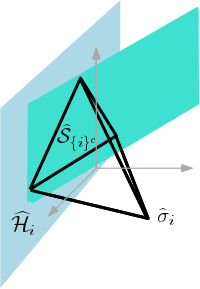
\includegraphics[scale=0.3]{Hin_plane}
		\subcaption{}
	\end{minipage}
	\begin{minipage}{0.45\textwidth}
	\centering
	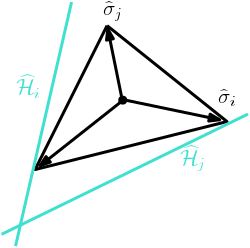
\includegraphics[scale=0.5]{Hin_plane2}
	\subcaption{}
\end{minipage}
\caption{An illustration of the fact that, in general, $\splxn_\ic$ is not contained in $\Hn_i=\{\x:\la \x,\svn_i^+\ra + \beta_i=0\}$. }
\label{fig:Hin_planes}
\end{figure}

We might expect that Lemma \ref{lem:SUn_subset} yields a hyperplane representation of the normalized simplex, as did Lemma \ref{lem:SUsubset} for the combinatorial simplex. Unfortunately however, the issue is once again complicated by the vertex weights and the relation between $\Svn^+$ and $\Svn$. Let us illustrate the problem by focusing on $\splxn$. 

As opposed to Section \ref{sec:S_G}, $\splxn_\ic $ is not contained in the hyperplane $\Hn_i = \{\x: \la \x,\svn_i^+\ra + \beta_i=0\}$, where we take $\beta_i = \beta_i^{\{i\}^c} = \sqrt{w(i)}\max_{j\neq i}\sqrt{w(j)} / \vol(G)$. To see this, take any $k\notin \argmax_{j\neq i} \sqrt{w(j)}$ (such a $k$ exists iff the graph is not regular) and note that while $\sv_k\in\splxn_U$ it is not in $\Hn_i$: 
\[\la \svn_k,\sv_i^+\ra = \bchi_k\Svn^\tp\Svn^+\bchi_i = -\frac{\sqrt{w(k)w(i)}}{\vol(G)}\neq \beta_i,\]
by assumption. The other way to see this is to note that $\svn_i^+$ is not perpendicular to $\splxn_\ic$ in general by Corollary \ref{cor:Sn_orthog_iff_regular}. Thus, it is not  clear how to generate an analogous description to Equation \eqref{eq:S_alt_desc} for the normalized simplex. While this may seem relatively inconsequential, it severely complicates finding the dual of $\splxn_G$, which is the question we turn to next. 

\paragraph{What is $\splxn_G^\du$ and and $(\splxn_G^+)^\du$?} 
Given that $\splxn_G^+$ is not the dual of $\splxn_G$ in general, it  seems appropriate  to  ask ``what on  earth \emph{is} the dual of the normalized simplex?". The question has an interesting  implicit answer when asked of  $\splxn_G^+$, as demonstrated by  the following  lemma. 

\begin{lemma}
	For any graph $G$, there  exists a graph $H$ such that the  dual  of $\splxn_G^+$ is the combinatorial  simplex of $H$.  
\end{lemma} 
\begin{proof}
Using the same reasoning which was applied to $\splx_G^+$, we see that $\splxn_G^+$  is also hyperacute.
This implies, by Theorem~\ref{thm:graph-simplex}, that its centred version is the inverse \emph{combinatorial} simplex of some graph $H$. That is,  $(\splxn_G^+)_0 = \splx_H^+$. Since all translationally congruent simplices  share the same dual, we have 
\begin{equation*}
(\splxn_G^+)^\du = (\splxn_G^+)^\du_0 = (\splx_H^+)^\du = \splx_H.\qedhere
\end{equation*}
\end{proof}

Unfortunately, this result is purely  existential and does not yield much insight as to  actual structure of $(\splxn_G^+)^\du$. In the  case of $\splxn_G$, somewhat surprisingly, the question is intimately related to the hyperplane representation---or lack thereof---of $\splxn_G$. 
We can obtain an implicit representation for the dual vertices $\{\svnd_i\}$ by noting that they must satisfy  $\la \svnd_i,\svn_j-\svn_n\ra=\delta_{ij}$ for all $i,j\neq n$. This translates to 
\begin{equation*}
\sum_{\ell=1}^n \svnd_i(\ell)(\vpn_k(j)-\vpn_k(n))\lambdan_k^{1/2}=\delta_{ij},
\end{equation*}
but extracting values of $\svnd_i$ which meet this condition is not trivial. 
We might, however, try a different tactic. Note that in the case of the combinatorial simplices, the dual vertices are encoded in their hyperplane representation by Equation \eqref{eq:S_alt_desc}: $\splx_G = \bigcap_i\{\x:\la \x,\sv_i^+\ra \geq -1/n\}$. It is thus  natural to wonder whether this relationship holds for every simplex, that is,  if given a simplex described as the intersection of haldspaces, say $\ssplx=\bigcap_i \{\x:\la \z_i,\x\ra \geq b_i\}$ are the vectors $\z_i$ are parallel to the dual vertices of $\ssplx$.  The following lemma gives gives sufficient conditions as to when this is the case. 

 
\begin{lemma}
	\label{lem:hdesc_dual}
	Let $\ssplx\subset\R^{n-1}$ be a centred simplex with $\ssplx=\bigcap_{i=1}^n  \{\x\in\R^{n-1}: \la \x,\z_i\ra \geq  \alpha_i\}$. Then $\{-\z_i/(\alpha_i n)\}$ are the vertices of $\ssplx^\du$. 
\end{lemma}
\begin{proof}
	As usual, let $\{\sv_i\}$ be the vertices of $\ssplx$. Put $\bgamma_i = -\z_i/(\alpha_i n)$. We need to show that $\{\bgamma_i\}_{i=1}^{n-1}$ is the sister basis to $\{\sv_i-\sv_n\}_{i=1}^{n-1}$. Let $H_i$ be the boundary of the halfspace $\{\x:\la \x,\z_i\ra \geq \alpha_i\}$, so $H_i = \{\x:\la \x,\z_i\ra = \alpha_i\}$. Enumerate the vertices $\{\sv_i\}$ such that $\splx_\ic \subset H_i$. Fix $i\in[n-1]$. We claim that 
	\[\sv_i \in \bigcap_{j\neq i}H_i.\]
	Indeed, $\splx_\jc$ is the $n-1$ dimensional simplex with vertices $\{\sv_\ell\}_{\ell\neq j}$. Hence $\sv_i\in \splx_\jc$ for all $j\neq i$ and thus also lies in $\cap_{j \neq i}H_j$. Therefore, $\la \sv_i,\z_j\ra = \alpha_j$ for all $j\neq i$, from which it follows  that $\la \bgamma_j,\sv_i-\sv_n\ra = -\la \z_j,\sv_i\ra/(\alpha_j n) + \la \z_j,\sv_n\ra / (\alpha_j n )=1/n - 1/n =0$.  
	It remains to show that $\la \bgamma_i,\sv_i-\sv_n\ra=1$ for all $i\neq n$. Since $\ssplx$ is centred by assumption, we have $\sv_i = -\sum_{j\neq i} \sv_j$. Consequently, 
	\begin{align*}
	\la \bgamma_i,\sv_i-\sv_n\ra &= -\sum_{j\neq i}\la \bgamma_i,\sv_j\ra - \la \bgamma_i,\sv_n \ra = \frac{1}{n}(n-1) + \frac{1}{n} = 1,
	\end{align*}
	as was to be shown.  
\end{proof}

Lemma \ref{lem:hdesc_dual} allows us to extract the dual given a hyperplane description of a centred simplex. The next natural question is then how the hyperplane description of an arbitrary simplex relates to the hyperplane description of its centred counterpart. This is answered by the following lemma. 

\begin{lemma}
	\label{lem:hdesc_centred}
	Let $\ssplx=\cap_i \{\x:\la \x,\z_i\ra \geq \alpha_i\}$ be a simplex. Its centred version, $\ssplx_0$, can be written as $\cap_i \{\x:\la \x,\z_i\ra \geq \alpha_i - \la \cent(\ssplx),\z_i\ra\}$. 
\end{lemma}
\begin{proof}
	As usual, take $\H_i = \{\x:\la \x,\z_i\ra = \alpha_i\}$ to be the hyperplanes bounding the simplex. The hyperplanes bounding the centred simplex, are parallel to the hyperplanes $\H_i$ and can thus be written as 
	\[\H_{i0} = \{\x:\la \x,\z_i\ra = \beta_i\},\]
	for some $\beta_i$. Moreover, just as $\sv_j\in\H_i$ for $j\neq i$, we have $\sv_j-\cent(\ssplx)\in \H_{i0}$, since $\{\sv_j-\cent(\ssplx)\}$ are the vertices of $\ssplx_0$. As such, $\la \sv_j-\cent(\ssplx),\z_i\ra=\beta_i$, and 
	\[\la \sv_j-\cent(\ssplx),\z_i\ra = \la \sv_j,\z_i\ra - \la\cent(\ssplx),\z_i\ra = \alpha_i - \la\cent(\ssplx),\z_i\ra,\]
	whence $\beta_i = \alpha_i - \la\cent(\ssplx),\z_i\ra$. It then follows that 
	\[\ssplx_0=\bigcap_i \H_{i0}^{\geq },\]
	where $\H_{i0}^\geq = \{\x:\la \x,\z_i\ra \geq  \alpha_i - \la \cent(\ssplx),
	\z_i\ra\}$. 
\end{proof}

Taken together, Lemmas \ref{lem:hdesc_dual} and \ref{lem:hdesc_centred} provide a path to try and determine the dual simplex of $\splxn_G$. In particular, if we could determine a hyperplane representation of any simplex congruent to $\splxn_G$,  then we can obtain a hyperplane representation of its centred version by Lemma \ref{lem:hdesc_centred} and to the dual of its centred version by Lemma \ref{lem:hdesc_dual}. Since the dual is common to all congruent simplices by Observation \ref{obs:dual_centred}, this would yield $\splx_G^\du$. Unfortunately, obtaining such a representation is  not trivial. We leave the question as an  open problem. 

 






\chapter{Further Properties of the Correspondence}
\label{chap:further_properties}

\chapterquote{Everything is  funny,  if you can laugh at it.}{Lewis Carroll}

The previous chapter introduced the graph-simplex correspondence and devoted several sections to the basic properties of the simplices associated to a given graph. In this chapter we  continue the study of the correspondence and present several of its more significant (but perhaps more complicated) properties.  We begin,  however, by demonstrating that  some of the interplay between $\splx_G$ and $\splx_G^+$ generalizes to an arbitrary simplex and its dual. 

\section{A General Property of the Dual Simplex }
Given that $\splx_G^+$  is the dual of $\splx_G$, it is natural to wonder whether some aspects of  their relationship are common to that between any simplex and its dual.  
Here we demonstrate that this is indeed the case; in particular, the Gram matrix of any (centred) simplex and its dual enjoy  the same pseudoinverse relationship. 
As we explained in Section~\ref{sec:Sn_G}, this relationship  is crucial to many of the proofs pertaining to  the combinatorial  simplices.
That  an equivalent property  holds for arbitrary simplices is therefore highly beneficial for their  study. 

\begin{lemma}
	\label{lem:dual_pseudoinverse}
	Let $\ssplx\subset\R^{n-1}$ be an arbitrary centred  simplex, and $\ssplx^\du$ its dual. Put $\Sv=\Sv(\ssplx)=(\bgamma_i)$ and $\Sv^\du=\Sv(\ssplx)=(\bgamma_i^\du)$ as usual. Then $\Sv^\du\Sv^\tp = \Sv(\Sv^\du)^\tp=\I$ and $(\Sv^\du)^\tp\Sv^\du$ is the Moore-Penrose pseudoinverse of $\Sv^\tp\Sv$. 
\end{lemma}
\begin{proof}
	First we inquire into the relationship between $\Sv$ and $\Sv^\du$. Put $\M=(\bgamma_1-\bgamma_n,\dots,\bgamma_{n-1}-\bgamma_n)$ and $\Q = (\bgamma^\du_1,\dots,\bgamma_{n-1}^\du)$. By definition, $\{\bgamma_i^\du\}$ is the dual  basis to $\{\bgamma_i-\bgamma_n\}$. Thus, by Observation~\ref{obs:bi-orthogonal_unique}, $\Q^\tp=\M^{-1}$ (we are working in $\R^{n-1}$), so  $\M\Q^\tp=\I$. The $(i,j)$-th component of this matrix product can therefore be expressed as 
	\begin{align}
	\delta_{ij} = \M\Q^\tp(i,j) &= \sum_{\ell=1}^{n-1} (\bgamma_\ell(i) - \bgamma_n(i))\bgamma_\ell^\du(j) = \sum_{\ell=1}^{n-1} \bgamma_\ell(i)\bgamma^\du_\ell(j) - \bgamma_n(i)\sum_{\ell=1}^{n-1}\bgamma^\du_\ell(j).\label{eq:lem_dual_pseudoinverse1}
	\end{align}
	Now,  since $\ssplx^\du$ is centred, 
	\begin{equation*}
	0=	(\Sv^\du\one)(j) = \sum_{\ell\in[n]} \bgamma_\ell^\du(j),
	\end{equation*}
	implying that $\sum_{\ell=1}^{n-1}\bgamma_\ell^\du(j) = - \bgamma_n^\du(j)$. Equation~\eqref{eq:lem_dual_pseudoinverse1} can then be written as 
	$
	\sum_{\ell=1}^{n} \bgamma_\ell(i)\bgamma_\ell^\du(j)=\delta_{ij},
	$
	implying that the components of $\Sv^\du\Sv^\tp$ are
	\begin{align*}
	(\Sv^\du\Sv^\tp)(i,j) &= \sum_{\ell=1}^n \bgamma_\ell^\du(i)\bgamma_\ell(j)=\delta_{ij},
	\end{align*}
	so that $\Sv^\du\Sv^\tp=\I$. A similar argument  holds for $\Sv(\Sv^\du)^\tp$, \emph{mutatis mutandis}.  
	
	We now proceed to demonstrating the pseudoinverse relation between $\Sv^\tp\Sv$ and $(\Sv^\du)^\tp\Sv^\du$. Recall that to demonstrate that  a matrix $\B_1$ is the pseudoinverse of $\B_2$, we need  to show that (i) $\B_1\B_2\B_1=\B_1$, (ii) $\B_2\B_1\B_2=\B_2$, (iii) $(\B_1\B_2)^\tp = \B_1\B_2$ and  (iv)  $(\B_2\B_1)^\tp = \B_2\B_1$ (Definition~\ref{def:simplex}). Using the relationship between  $\Sv^\du$ and  $\Sv$ given above, these become simple computations. For instance, 
	\begin{equation*}
	\Sv^\tp\Sv(\Sv^\du)^\tp\Sv^\du\Sv^\tp\Sv = \Sv^\tp \I^2 \Sv=\Sv^\tp\Sv,
	\end{equation*}
	and, 
	\begin{align*}
	((\Sv^\du)^\tp\Sv^\du \Sv^\tp\Sv)^\tp = ((\Sv^\du)^\tp\I\Sv)^\tp = \Sv^\tp\Sv^\du = \I-\frac{\J}{n} = (\Sv^\du)^\tp\Sv = (\Sv^\du)^\tp\I\Sv = (\Sv^\du)^\tp\Sv^\du\Sv^\tp\Sv.
	\end{align*} 
	Conditions (i) and (iii) therefore  hold between $\Sv^\tp\Sv$ and  $(\Sv^\du)^\tp\Sv^\du$; conditions (ii) and (iv) follow similarly. 
\end{proof}


In the next  section, we  will demonstrate  that this insight allows us to  generalize results pertaining to hyperacute simplices to all simplices. 
We thus witness another benefit of the correspondence: By leveraging knowledge  of $\splx_G$ and $\splx_G^+$ we  can  gain insights into the behaviour of general simplices. 



\section{Block Matrix Equations}
\label{sec:block_matrix}
In this section we are finally able  to satisfy those readers who have  wondered about the applicability of electrical  networks to the graph-simplex correspondence. Applying Lemma~\ref{lem:block_equation_graph}, we are able to  develop block matrix equations which relate the structure of $\splx_G$ and $\splx_G^+$. Then,  using the results of the previous section we generalize  these equations to arbitrary simplices.  

Before we  begin, a brief remark on the relationship of the following results  and Fiedler's work. Fiedler's derivation of the graph-simplex correspondence relied on a matrix equation---an equation equivalent to~\eqref{eq:simplex_block_matrix}, in fact~\cite[Theorem 3.1]{fiedler1993geometric}. Conversely, we are obtaining such equations as a \emph{consequence} of the correspondence. It is our hope that different treatments of the material shed light on its different---and hopefully complementary---implications.  

Let a centred, hyperacute simplex $\ssplx$ be given, with $\Sv(\ssplx)=\{\bgamma_i\}$.  Let $\bar{d}$ be the average squared distance between all the vertices of $\ssplx$, that is
\begin{equation}
\label{eq:avg_squared_distance}
\bar{d} \equiv  \frac{1}{n^2}\sum_{i\leq j} \norm{\bgamma_i-\bgamma_j}_2^2.
\end{equation}
Let $\xi(i)$ give the average squared distance of vertex $i$ from other vertices minus the total average distance, 
\begin{equation}
\label{eq:avg_sqd_distance_i}
\xi(i) \equiv \frac{1}{n}\sum_{j} \norm{\bgamma_i-\bgamma_j}_2^2 - \bar{d},
\end{equation}
and put $\bxi=(\xi(1),\dots,\xi(n))$. 
The following  results relate  the distance matrix of $\ssplx$ to the vertex  matrix of its dual. 

\begin{lemma}
	\label{lem:block_inverse_simplex}
	Let $\ssplx\subset\R^{n-1}$ be a hyperacute simplex with  squared distance matrix $\D_\ssplx$, and average squared distance vector $\bxi$.
	Let $\Q=(\Sv^\du)^\tp\Sv^\du$  where $\Sv^\du$ is the vertex matrix of $\ssplx^\du$.  Then, 
	\begin{equation}
	\label{eq:simplex_block_matrix}
	-\frac{1}{2} \begin{pmatrix}
	0 & \one_n^\tp \\ 
	\one_n &  \D_\ssplx
	\end{pmatrix} = \begin{pmatrix}
	\bxi^\tp \Q\bxi + 4\overline{d} & -(\Q\bxi + 2\one/n)^\tp \\
	-(\Q\bxi + 2\one/n) & \Q
	\end{pmatrix}^{-1}.
	\end{equation}
	Moreover, the vertices of $\ssplx^\du$ and the distance matrix of $\ssplx$ are related by the equation
	\begin{equation}
	\label{eq:lem_inverse_relation}
	\Q \D_\ssplx \Q = -2\Q,
	\end{equation}
	and in the space $\spn(\one)^\perp$ it holds that 
	\begin{equation*}
	\label{eq:lem_inverse_relation2}
	\D_\ssplx\Q \D_\ssplx= -2\D_\ssplx.	
	\end{equation*}
\end{lemma}

\begin{proof}
By Theorem~\ref{thm:graph-simplex}, $\ssplx$ is the inverse simplex of some graph $G$ and therefore $\D=\D_\ssplx=\Reff$, where $\Reff$ is the effective resistance matrix (Lemma~\ref{lem:S_G_basic_properties}). Therefore, we can rewrite $\xi(i)$ as 
 \begin{align*}
\frac{1}{n}\sum_j \effr(i,j) - \frac{1}{n^2}\sum_{i<j}\effr(i,j),
\end{align*}
whence,
\begin{align*}
\bxi = \frac{1}{n}\Reff\one - \frac{1}{n^2} \one \one^\tp \Reff\one = \frac{1}{n}\Reff\one - \frac{1}{n^2} \J \Reff\one.
\end{align*}
Meanwhile, the dual simplex to $\ssplx$ is the simplex of the graph $G$, and hence obeys $\Q=\L_G$. Consequently, letting $\bD=\frac{1}{n}\Reff\one - \frac{1}{n^2} \J \Reff\one$, we can rewrite Equation~\eqref{eq:simplex_block_matrix} as the purely graph theoretic statement  
\begin{equation*}
%\label{eq:block_inverse_er}
	-\frac{1}{2} \begin{pmatrix}
0 & \one_n^\tp \\ 
\one_n &  \Reff
\end{pmatrix} = 
\begin{pmatrix}
\bD^\tp \L_G\bD + \frac{4}{n^2}\Rtot_G & -(\L_G\bD + \frac{2}{n}\one)^\tp \\
-(\L_G\bD + \frac{2}{n}\one) & \L_G
\end{pmatrix}^{-1}.
\end{equation*}
This equation is verified by Lemma~\ref{lem:block_equation_graph}. The final two equations in  the lemma translate to $\L_G\Reff_G\L_G=-2\L_G$ and $\Reff_G\L_G\Reff_G=-2\Reff_G$ on $\spn(\one)^\perp$. Both of these also hold  via Lemma~\ref{lem:block_equation_graph}. 
\end{proof}


While Lemma~\ref{lem:block_inverse_simplex} may be interesting, it is unfortunately restricted in its scope. In what follows we demonstrate that it can be generalized to hold for all simplices. Before we begin, we require a generalization of the statement $\Reff=\bD\one^\tp+\one\bD^\tp - 2\L_G^+$ to all distance  matrices (recall  that $\Reff$ is the  distance  matrix of $\splx_G^+$). This is accomplished by  the following lemma. 


\begin{lemma}
	\label{lem:distance_matrix}
	For any centred simplex $\ssplx\subset\R^{n-1}$  with distance matrix $\D_\ssplx$ and vertex  matrix $\Sv$, it holds  that $\D_\ssplx = \one\bxi^\tp + \bxi\one^\tp - 2\Sv^\tp\Sv$.
\end{lemma}
\begin{proof}
	Fix  $k,\ell\in[n]$. The proof is purely computational. We have 
	\begin{equation*}
	(\bxi\one^\tp)(k,\ell) = \frac{1}{n}\sum_j\norm{\bgamma_k-\bgamma_j}_2^2 - \bar{d},\quad (\one\bxi^\tp)(k,\ell) = \frac{1}{n}\sum_j\norm{\bgamma_\ell-\bgamma_j}_2^2 - \bar{d}, 
	\end{equation*}
	and  $-2\Sv^\tp\Sv = -2\la \bgamma_k,\bgamma_\ell\ra$. 
	Expanding the norm in terms of dot products, write
	\begin{align*}
	(\bxi\one^\tp + \one\bxi^\tp - 2\Sv^\tp\Sv)(k,\ell) &= \frac{1}{n}\bigg(\sum_j \norm{\bgamma_k-\bgamma_j}_2^2 + \sum_j\norm{\bgamma_\ell-\bgamma_j}_2^2 \bigg) \\
	&\qquad- \frac{2}{n^2}\sum_{i<j} \norm{\bgamma_i-\bgamma_j}_2^2 -2\la\bgamma_k,\bgamma_\ell\ra \\ 
	&=\frac{1}{n}\sum_j\left(\norm{\bgamma_k}_2^2 + \norm{\bgamma_j}_2^2+\norm{\bgamma_\ell}_2^2 +\norm{\bgamma_j}_2^2  -2\la \bgamma_k,\bgamma_j\ra -2\la\bgamma_\ell,\bgamma_j\ra\right) \\
	&\qquad -\frac{1}{n^2}\sum_{i,j}\left(\norm{\bgamma_i}_2^2+\norm{\bgamma_j}_2^2-2\la\bgamma_i,\bgamma_j\ra\right)  -2\la \bgamma_k,\bgamma_\ell\ra. \\
	&= \norm{\bgamma_k}_2^2 + \norm{\bgamma_\ell}_2^2 - 2\la\bgamma_k,\bgamma_\ell\ra + 2\bigg(\frac{1}{n}\sum_j\norm{\bgamma_j}_2^2 - \frac{1}{n^2}\sum_{i,j}\norm{\bgamma_j}_2^2\bigg)  \\
	&\qquad +\frac{1}{n^2}\sum_{i,j} \la \bgamma_i,\bgamma_j\ra - \frac{2}{n}\sum_j (\la \bgamma_k,\bgamma_j\ra -\bgamma_\ell,\bgamma_j\ra).
	\end{align*} 
	Note that in the second  line we removed the factor of two from $\bar{d}$ by summing over all $i,j$ rather than simply $i<j$. 
	Now, the first three terms in the final equation are  equal to $\norm{\bgamma_k-\bgamma_\ell}_2^2=\D_\ssplx(k,\ell)$. Therefore,  it remains  to show  that the final  three terms are zero. The first  of  these, $\frac{1}{n}\sum_j\norm{\bgam_j}_2^2 - \frac{1}{n^2}\sum_{i,j}\norm{\bgamma_j}_2^2$,  is clearly   zero after noticing that the final summand is independent of $i$. As for the final two, we write them in terms of  the centroid of $\ssplx$ (which is $\zero$), as 
	\begin{align*}
	&\quad \frac{1}{n^2}\sum_{i,j} \la \bgamma_i,\bgamma_j\ra - \frac{2}{n}\sum_j (\la \bgamma_k,\bgamma_j\ra -\bgamma_\ell,\bgamma_j\ra) \\
	&= \frac{1}{n^2}\bigg\la \sum_i\bgamma_i,\sum_j\bgamma_j\bigg\ra - \frac{2}{n}\bigg(\bigg\la \bgamma_k,\sum_j\bgamma_j\bigg\ra 
	 -\bigg\la \bgamma_\ell,\sum_j\bgamma_j\bigg\ra\bigg) \\
	&= \frac{1}{n^2}\la n\cent(\ssplx),n\cent(\ssplx)\ra - \frac{2}{n}(\la \bgamma_k,n\cent(\ssplx)\ra - \la \bgamma_\ell,n\cent(\ssplx)\ra \\
	&= 0,
	\end{align*}
	as was to  be shown. 
\end{proof}

We can now strengthen  Lemma~\ref{lem:block_inverse_simplex} to all simplices,  even those which  are not centred.   

\begin{theorem}
	\label{thm:block_general_simplex}
	The equations of Lemma~\ref{lem:block_inverse_simplex} hold for \emph{any} simplex $\ssplx\subset\R^{n-1}$. 
\end{theorem}
\begin{proof}
	Let us first assume that $\ssplx$ is centred. 
	The proof proceeds very much as  does  that of Lemma~\ref{lem:block_equation_graph}, by computing the matrix product  
	\[\begin{pmatrix}
	0 & \one^\tp \\
	\one & \D_\ssplx
	\end{pmatrix} \begin{pmatrix}
	\bxi^\tp\Q\bxi + 4\bar{d}  &  -(\Q\bxi  + \frac{2}{n}\one)^\tp  \\
	-(\Q\bxi  + \frac{2}{n}\one) &  \Q
	\end{pmatrix},\] and demonstrating that it equals $-2\I$. Instead of leverage  the relationship $\Reff_G=\one\bD^\tp+\bD\one^\tp - 2\L_G^+$ as was done  in that case, we use the more general equation $\D_\ssplx = \one\bxi^\tp+\bxi\one^\tp - 2\Sv^\tp\Sv$ given by Lemma~\ref{lem:distance_matrix}. However, since that proof  was given  in the appendix we will give this one here.  The top left corner of  the product of these two matrices is $-\one^\tp\Q\bxi-2/n \one^\tp\one = -2$ as $\one^\tp\Q = \one^\tp(\Sv^\du)^\tp\Sv^\du$ since $\ssplx^\du$ is centred by definition. Likewise,  the top right  hand corner is zero.  After expanding $\D_\ssplx$  in accordance with Lemma~\ref{lem:distance_matrix} the bottom left  corner becomes 
	\begin{align}
	&\one\bxi^\tp\Q\bxi+4\bar{d}\one - (\one\bxi^\tp+\bxi\one^\tp - 2\Sv^\tp\Sv)\Q\bxi -\frac{2}{n}\D_\ssplx\one = 4\bar{d}\one + 2\Sv^\tp\Sv\Q\bxi  -\frac{2}{n}\D_\ssplx\one. \label{eq:lem_block_general_simplex1}
	\end{align}
	Lemma~\ref{lem:dual_pseudoinverse} dictates that $\Q$ is the pseudoinverse of $\Sv^\tp\Sv$ so, by Lemma~\ref{lem:pseudoinverse_properties}, $\Sv^\tp\Sv\Q=\I-\J/n$ (of course, we're implicitly using that $\spn(\one)^\perp = \ker(\Sv)=\ker(\Sv^\tp\Sv)$). 
	Moreover, after noting that 
	\begin{equation*}
	\bxi = \frac{1}{n}\D_\ssplx\one -\bar{d}\one,\quad \text{and}\quad  \bar{d} = \frac{1}{2n^2}\one^\tp\D\one,
	\end{equation*}
	we can  rewrite the right  hand side of Equation~\eqref{eq:lem_block_general_simplex1} as 
	\begin{align*}
	&\quad  4\bar{d}\one +2\bigg(\I-\frac{\J}{n}\bigg)\bigg(\frac{1}{n}\D_\ssplx\one-\bar{d}\one\bigg)  -\frac{2}{n}\D_\ssplx\one \\
	&= 2\bar{d}\one -  \frac{2}{n^2}\J\D_\ssplx\one + \frac{2}{n}\J\bar{d}\one \\
	&=\frac{1}{n^2}\J\D_\ssplx\one -  \frac{2}{n^2}\J\D_\ssplx\one + \frac{1}{n^3}\J^2\D_\ssplx\one \\
	&= \frac{1}{n^2}\J\D_\ssplx\one -  \frac{2}{n^2}\J\D_\ssplx\one + \frac{1}{n^2}\J\D_\ssplx\one=\zero.
	\end{align*}
	Carrying out a similar  procedure for  the  bottom right corner, we  obtain  
	\begin{align*}
	-\one\bxi^\tp\Q-\frac{2}{n}\J+\D_\ssplx\Q &= -\one\bxi^\tp\Q-\frac{2}{n}\J  + (\one\bxi^\tp+\bxi\one^\tp -2\Sv^\tp\Sv)\Q \\
	&= -\frac{2}{n}\J-2\bigg(\I-\frac{\J}{n}\bigg) = -2\I.
	\end{align*}
	The  final two equations follow via similar computations: 
	\begin{align*}
	\Q\D_\ssplx\Q = \Q(\one\bxi^\tp+\bxi\one^\tp-2\Sv^\tp\Sv)\Q = -2\Q\Sv^\tp\Sv\Q = -2\Sv^\tp\Sv,
	\end{align*}
	due to properties of the pseudoinverse (Lemma~\ref{lem:pseudoinverse_properties}), and if $\x\perp\one$ then 
	\begin{align*}
	\D_\ssplx \Q\D_\ssplx \x = \D_\ssplx \Q(\one\bxi^\tp  +\bxi\one^\tp - 2\Sv^\tp\Sv)\x = -2\D_\ssplx\Q \Sv^\tp\Sv\x = -2\D_\ssplx\bigg(\I-\frac{\J}{n}\bigg) \x = -2\D_\ssplx,
	\end{align*}
	which completes the proof if $\ssplx$ is centred. If $\ssplx$  is not centred, then we need only apply the relationship to its centred  version $\ssplx_0$, and note  that the quantities $\D_\ssplx, \bxi,\bar{d}$ and $\Q$ are the same for $\ssplx_0$ and $\ssplx$. The first three are the same because they deal with distances between vertices, which are invariant under linear transformations. $\Q$ is the  same due to  Observation~\ref{obs:dual_centred}. 
\end{proof}

\begin{remark}
	We have thus recovered Fiedler's block matrix relation~\cite{fiedler1993geometric}, although he does not give the same explicit   interpretation of  the entries as we do. As discussed above, it is interesting that Fiedler used the equation  as the basis for the correspondence while our approach is the reverse. 
\end{remark}

\subsection{Applications}
We now discuss several  uses of the equations developed above. 
One consequence is a relation between the volume of the simplex and the effective resistances in the graph. To see this, we need to introduce a particular object from the field of distance geometry. Let $\D(\X)$ be the distance matrix of a set $\X$ of $d$ points. The matrix 
\begin{equation}
\label{eq:menger_matrix}
\begin{pmatrix}
0 & \one^\tp \\
\one & \D(\X)
\end{pmatrix}\in\R^{(d+1)\times (d+1)},
\end{equation}
is called the \emph{Menger matrix of $X$}, the determinant of which is called the \emph{Cayley-Menger determinant}, named after Arthur Cayley and Karl Menger~\cite{cayley1841theorem, Menger1928}. The Cayley-Menger determinant is related to the volume of the underlying set of points as follows. 


\begin{lemma}[\cite{menger1931new}]
	\label{lem:menger_volume}
	Let $\D(\X)$ be the distance matrix of a set $\X$ of $d$ points. The squared $d-1$ dimensional volume\footnote{That is, the volume as calculated in $\R^{d-1}$.} of the convex hull of $\X$ is proportional to the  determinant of the Menger matrix: 
	\begin{equation}
	\label{eq:vol(convX)}
	\vol^2(\conv(\X)) = \frac{(-1)^d}{((d-1)!)^2 2^{d-1}} \det\begin{pmatrix}
	0 & \one^\tp \\
	\one & \D(\X)
	\end{pmatrix}.
	\end{equation} 
\end{lemma}

The relation between the Menger matrix and the volume combined with the matrix equations above allows us to give a concise formula for the volume of any hyperacute simplex. 
This fact  was first pointed out by Van Mieghem \etal~\cite{van2017pseudoinverse}. 

\begin{lemma}
	\label{lem:volume}
	Let $\splx^+\subset\R^{n-1}$ be the inverse combinatorial simplex of $G$. The  $n-1$ dimensional volume of $\splx^+$ is
	\begin{equation}
	\label{eq:vol(T)}
	\vol(\splx^+) = \frac{1}{(n-1)!\cdot \Gamma_G^{1/2}},
	\end{equation}
	where $\Gamma_G$ is the total weight of all spanning  trees of $G$. 
\end{lemma}

We remind the reader that $\Gamma_G$ was discussed in  Section~\ref{sec:background_laplacian}; see  Equation~\eqref{eq:Gamma_G}  in particular. The proof of Lemma~\ref{lem:volume} may  be  found in Appendix~\ref{sec:app_proofs_further}.   


We can use these results to produce an  equation relating the  diagonal entries of the Laplacian to the volume of $\splx_G^+$ and its facets.  

\begin{lemma}
	\label{lem:L(i,i)_trees}
	Let $G$ be a connected graph and fix $i\in V(G)$. 
	Put $G_\ic=G[V\setminus \{i\}]$. If $\splx^+\subset\R^{n-1}$  is the inverse combinatorial simplex of $G$ then the volumes
	of $\splx^+_\ic$ and $\splx^+$ are related as 
	\begin{equation}
	\label{eq:vol/vol}
	\frac{\vol^2(\splx_\ic^+)}{\vol^2(\splx^+)} = (n-1)^2\L_G(i,i) = (n-1)^2w(i).
	\end{equation}
\end{lemma}
\begin{proof}
	Let $\splx^+$ have vertices $\sv_1^+,\dots,\sv_n^+$, and let $\M$ be the Menger matrix associated with $\splx^+$. Sylvester's formula (Lemma~\ref{lem:sylvester}) gives us that 
	\begin{equation*}
	\M^{-1}(i+1,i+1) =\det\M^{-1}(i+1,i+1)= \pm \frac{\det\M(U,U)}{\det\M},
	\end{equation*}
	where $U=\{i+1\}^c$. Observe that $\M(U,U)$ is the Menger matrix of the simplex $\splx_\ic^+$; we are simply removing the row and column corresponding to the $i$-th vertex. Translating the determinants of Menger matrices into statements about volumes of simplices via Equation~\eqref{eq:vol(T)} gives 
	\begin{align*}
	\M^{-1}(i+1,i+1) &= \pm \frac{[(n-2)!]^2 2^{n-2}}{(-1)^{n-1}}\vol^2(\splx_\ic^+) \bigg / \frac{[(n-1)!]^2 2^{n-1}}{(-1)^n} \vol^2(\splx^+) \\
	&= \mp \frac{1}{2(n-1)^2}\frac{\vol^2(\splx_\ic^+)}{\vol^2(\splx^+)}. 
	\end{align*} 
	Via the block matrix equation~\eqref{eq:block_inverse_er} we have $\M^{-1}(i+1,i+1) = -\frac{1}{2}\L_G(i,i)$ (since the distance matrix  of $\splx^+$  is the effective resistance matrix of $G$). Plugging this into the above equation and noting that both $\L_G(i,i)$ and $\vol^2(\splx_\ic^+)/(2(n-1)^2\vol^2(\splx^+))$ are positive  gives the desired result. 
\end{proof}

\begin{remark}
	The facet  $\splx_\ic^+$ is distinct from the inverse combinatorial  simplex of the graph  $G_\ic$. However, if one could relate  their volumes then this would yield an equation for  $\L_G(i,i)$ in terms of the spanning trees of $G$ and  $G_\ic$ by combining Lemma~\ref{lem:volume}  and Equation~\eqref{eq:vol/vol}.  
\end{remark}

Given that Lemma~\ref{lem:volume} uses the block matrix equation  for hyperacute simplices, it  is natural  to wonder whether we  can generalize the result by appealing instead to generalized matrix equation which holds for all simplices  (Theorem~\ref{thm:block_general_simplex}). We can in fact, but first  we need to prove several results concerning the Gram matrix of a  general  dual  simplex.  We begin  with two  technical lemmas which  will later prove useful. 

\begin{lemma}
	\label{lem:volume_cofactors}
	For any simplex $\ssplx\subset\R^{n-1}$, let $\Q=\Sv(\ssplx^\du)^\tp\Sv(\ssplx^\du)$ be the Gram matrix of the dual simplex. The volume of $\ssplx$ is related  to  the cofactors of $\Q$ as 
	\begin{equation*}
	\vol^2(\ssplx) = \frac{4}{[(n-1)!]^2} \bigg(\sum_{i\in[n]}\sum_{j\in[n]} \r(i)\r(j)(-1)^{i+j}\det(\Q_{-i,-j})\bigg)^{-1},
	\end{equation*}
	where $\r=-\Q\bxi-\frac{2}{n}\one$. 
\end{lemma}
\begin{proof}
	The statement  is essentially  extracted from the proof of Lemma~\ref{lem:volume}, so we do not reformulate it here. We do  note, however, that this lemma makes use of the block matrix equation for general simplices, whereas the proof of Lemma~\ref{lem:volume}  relies  only on Lemma~\ref{lem:block_inverse_simplex}. 
\end{proof}

The following second technical lemma will help with our eventual aim of demonstrating  that all cofactors of a Gram matrix (of a centred simplex) are constant. The  previous lemma will then  enable us  to relate this value to the volume. 

\begin{lemma}
	\label{lem:cofactors_technical}
	Let  $\M\in\R^{n\times n}$ have real eigenvalues $\mu_1,\dots,\mu_n$. Then 
	\begin{equation}
	\label{eq:cofactors_technical}
	\sum_{i=1}^n \prod_{j\neq i}\mu_i = \sum_{i=1}^n  \det(\M_{-i,-j}).
	\end{equation}
\end{lemma}
\begin{proof}
We make use of technique used by Godsil and Royle~\cite{godsil2013algebraic} to prove Kirchoff's matrix  tree theorem. For $\M'$ and  $\M''$  square, it  holds that $\det(\M'+\M'') = \sum_{U\subset[n]} \det \M'_U$, where  $\M'_U$ is the matrix obtained by replacing row $i$  in $\M'$ with row   $i$ of $\M''$  for  all $i\in U$. We will apply  this to the sum $t\I-\M$. Fix $U\subset[n]$ and  let  us consider $\det(t\I)_U$ for a moment. Letting $S_n$ denote the set of all permutations on $n$ vertices,  recall  that the determinant obeys  
\begin{equation*}
\det((t\I)_U) = \sum_{\tau\in S_n}\sgn(\tau)\prod_{i\in[n]}(t\I)_U(i,\tau(i)),
\end{equation*}
where $\sgn(\tau)$ is the  sign  of the permutation. Now,  for  $i\notin  U$, the $i$-th row of $t\I$ is $t\e_i$, so $(t\I)_U(i,\tau(i)) = t\delta_{i,\tau(i)}$. Consequently, we can restrict  our attention to those permutations which fix each $i\notin U$: 
\begin{align*}
\det((t\I)_U) &= \sum_{\substack{\tau \in S_n\\\tau(i)=i,i\in U^c}} \sgn(\tau) \prod_{j\in U} (t\I)_U(j,\tau(j))\prod_{i\notin U}(t\I)_U(i,\tau(i)) \\
&=  \sum_{\substack{\tau \in S_n\\\tau(i)=i,i\in U^c}} \sgn(\tau) \bigg(\prod_{j\in U} (t\I)_U(j,\tau(j))\bigg)t^{n-|U|} \\
&= t^{n-|U|}\sum_{\tau \in S_{U}} \sgn(\tau) \prod_{j\in U} (-\M)(j,\tau(j)) \\
&= t^{n-|U|} \det(-\M(U,U)),  %= t^{n-|U|}(-1)^{|U|}\det(\Ln(U,U)).
\end{align*}
where we recall that $\M(U,U)$ denotes the submatrix of $\M$ indexed by the rows and columns of  $U$. It is worth remarking that the penultimate inequality follows because the  set of all permutations in $S_n$ which fix the elements of $U^c$ (i.e.,  do  not  change their positions) is in  one-to-one correspondence with the set of all permutations on $U$. The final equality then  uses the definition of the determinant. 
Returning to the characteristic polynomial, and noting that $\det(-\M(U,U))=(-1)^{|U|}\det(\M(U,U))$ write 
\begin{align}
\det(t\I - \M) &= \sum_{U\subset[n]} \det((t\I)_U) = \sum_{U\subset[n]}t^{n-|U|}(-1)^{|U|} \det(\M(U,U)) \notag \\
&=\sum_{k=1}^n \sum_{U\subset[n],|U|=k}t^{n-k}(-1)^k\det(\M(U,U)).\label{eq:lem_prod_evalsn1}
\end{align}
On the other  hand, we can of course  write the characteristic polynomial in  terms of  the  eigenvalues of $\M$~\cite{brooks2006coefficients}: 
\begin{align}
\det(t\I -\M) &= \sum_{k=0}^n (-1)^{n-k}\bigg(\sum_{U\subset[n],|U|=k}\prod_{i\in U}\mu_i\bigg)t^{n-k}.\label{eq:lem_prod_evalsn2}
\end{align}
Matching  the coefficients of the term involving  $t$  in  Expressions~\eqref{eq:lem_prod_evalsn1} and~\eqref{eq:lem_prod_evalsn2} gives 
\begin{align*}
(-1)^{n-1}\sum_{U\subset[n],|U|=n-1}\prod_{i\in U}\mu_i &= (-1)^{n-1}\sum_{U\subset[n],|U|=n-1}\det(\M(U,U)) \\
&= (-1)^{n-1}\sum_{i=1}^n\det(\M_{-i,-i}),
\end{align*}
which  is equivalent to the desired expression. 
\end{proof}


We are  now almost ready to prove  that all cofactors of Gram  matrices of dual simplices are equal. We require one final tool,  however.  
Let $\M\in\R^{n\times n}$. The \emph{adjugate} of $\M$, denoted by $\adj(\M)$, is the matrix whose $(i,j)$-th entry is equal to the $(j,i)$-th  cofactor of $\M$, i.e., 
\begin{equation*}
\adj(\M)(i,j) = (-1)^{i+j}\det(\M_{-i,-j}),
\end{equation*}
where $\M_{-i,-j}\in\R^{(n-1)\times( n-1)}$ is the matrix obtained by removing the $i$-th row and column of $\M$. The adjugate obeys  the following equation  (see e.g., \cite{godsil2013algebraic})
\begin{equation}
\label{eq:MadjM}
\M\adj(\M)=\det(\M)\I.
\end{equation}

\begin{lemma}
	\label{lem:cofactors_equal}
	Let $\BGamma$ be the vertex matrix of $n$ affinely independent points in  $\R^{n-1}$ whose  centroid is $\zero$,  i.e., $\BGamma\one=\zero$. Then (i) the cofactors of the Gram matrix  $\Q=\BGamma^\tp\BGamma$ are all equal to some number $\kappa(\Q)$ and (ii) $\prod_{i<n}\mu_i = n\cdot \kappa(\Q)$  where $\mu_1,\dots,\mu_{n-1}$ are the non-zero eigenvalues of $\Q$. 
\end{lemma}
\begin{proof}
	Note that $\det\Q=\zero$ since  $\one\in\ker\Q$. Hence, using Equation~\eqref{eq:MadjM}, $\Q\adj\Q = \det(\Q)\I=\zero_{n\times n}$. Each column  of $\adj\Q$ is  thus in $\ker\Q=\ker\BGamma=\spn(\one)$ (here we're using both  Lemma~\ref{lem:rank(QtQ)} and the fact that $\dim\ker\BGamma=1$ due to affine independence). Therefore, $\adj\Q = (\alpha_1\one,\alpha_2\one,\dots,\alpha_n\one)$ for some $\alpha_i\in\R$. However, since  $\Q$ is symmetric, $\Q_{-i,-j}=\Q_{-j,-i}$ for each $i,j\in[n]$, implying that $\adj\Q = (\adj\Q)^\tp$. This in turn implies that $\alpha_i=\alpha_j$  for all $i,j$, meaning that $\adj\Q$ is a constant matrix equal to, say, $\kappa(\Q)\J$. This proves (i). (ii) now follows from applying  Lemma~\ref{lem:cofactors_technical} along with the fact that  since $\Q$ has rank $n-1$, it has $n-1$ non-zero eigenvalues. Hence, if $\mu_n$  is the single zero eigenvalue, 
	\begin{equation*}
	\prod_{j<n}\mu_j = \sum_{i=1}^n \prod_{j\neq i}\mu_i = \sum_i \det(\Q_{-i,-i}) = n\kappa(\Q).\qedhere 
	\end{equation*}
\end{proof}


Finally, we can  extract a general theorem about the volume of arbitrary simplices.  


\begin{theorem}
	\label{thm:simplex_volume}
	For any simplex $\ssplx\subset\R^{n-1}$, 
	\begin{equation*}
	\vol(\ssplx) = \frac{\sqrt{n}}{(n-1)!}\prod_{i<n}\frac{1}{\mu_i^{1/2}},
	\end{equation*}
	where $\mu_1,\dots,\mu_{n-1}$ are the non-zero eigenvalues of the matrix   $\Q=\Sv(\ssplx^\du)^\tp\Sv(\ssplx)$, the Gram matrix of the dual simplex. 
\end{theorem}
\begin{proof}
As per Lemma~\ref{lem:cofactors_equal}, let the cofactors of  $\Q$ be  equal to $\kappa(\Q)$. Take  $\r=-\Q\bxi-\frac{2}{n}\one$  as usual.  
Combining Lemmas~\ref{lem:volume_cofactors} and~\ref{lem:cofactors_technical} gives  
\begin{align*}
\vol^2(\ssplx) &= \frac{4}{[(n-1)!]^2}\bigg(\kappa(\Q)\sum_{i,j\in[n]} r(i)r(j)\bigg)^{-1} \\
&= \frac{4}{[(n-1)!]^2\kappa(\Q)}(\la \r,\one\ra^2)^{-1} = \frac{n}{[(n-1)!]^2\prod_{i<n}\mu_i},
\end{align*}
where we've written $\kappa(\Q)$ in terms of the eigenvalues by Lemma~\ref{lem:cofactors_equal} and used that $\la \r,\one\ra = -2$. 
\end{proof}

As an immediate consequence of this theorem, we obtain the volume of the combinatorial simplex of a graph. Our  result matches  that obtained by Van Mieghem \etal~\cite{van2017pseudoinverse}, but is gleaned  in a  different manner. 

\begin{corollary}
	\label{cor:vol(SG)}
	For a connected graph $G$, 
	\begin{equation*}
	\vol(\splx_G) = \frac{\sqrt{n}}{(n-1)!}\prod_{i<n}\lambda_i^{1/2}  = \frac{n \cdot\Gamma_G^{1/2}}{(n-1)!}
	\end{equation*}
	where  $\lambda_1\geq \lambda_2\geq \dots\geq\lambda_{n-1}>  \lambda_n=0$  are the eigenvalues of $\L_G$. 
\end{corollary}
\begin{proof}
	The Gram matrix of the dual simplex of $\splx_G$ is $\L_G^+$,  which has eigenvalues $\lambda_i^{-1}$. Apply  Theorem~\ref{thm:simplex_volume}. The second  inequality follows from applying the matrix tree theorem.  
\end{proof}

Another consequence relates the volumes of the combinatorial simplices to the weight  of all spanning trees of $G$.  

\begin{corollary}
	\label{cor:vol(SG)/vol(S+)}
	The ratio of $G$'s combinatorial simplices  obeys
	\begin{align*}
	\frac{\vol(\splx_G)}{\vol(\splx_G^+)} = n\Gamma_G. 
	\end{align*}
\end{corollary} 
\begin{proof}
	We have $\vol(\splx_G) = \frac{\sqrt{n}}{(n-1)!}\prod_{i<n}{\lambda_i^{1/2}}$ and  $\vol(\splx_G^+) = \frac{\sqrt{n}}{(n-1)!}\prod_{i<n}{\lambda_i^{-1/2}}$. Take the  ratio   and recall that $\Gamma_G = \prod_{i<n}\lambda_i$.  
\end{proof}

Unfortunately,   it is  difficult to  garner  similar insights regarding the  normalized simplices. Indeed, because we do  not know what the duals of the normalized simplices are in general,  we cannot relate their volumes to the eigenvalues of $\Ln_G$. We can however, relate  the eigenvalues of $\Ln_G$ to the volumes of $\splx_G$ and  $\splx_G^+$.  To  do  this, we first need  to make a detour to  study the adjugate the normalized Laplacian. 

It is well-known  that the adjugate is commutative with matrix multiplication~\cite{godsil2013algebraic}: $\adj(\M\Q) = \adj(\M)\adj(\Q)$ for any $\M$ and  $\Q$. Applying this  to $\Ln$ (we drop the subscript), we have 
\begin{align*}
\adj(\Ln) &= \adj(\W^{-1/2}\L_G\W^{-1/2}) \\
&= \adj(\W^{-1/2})\adj(\L_G)\adj(\W^{-1/2}) \\
&= \Gamma_G \cdot \adj(\W^{-1/2})\,\J\,\adj(\W^{-1/2}),
\end{align*}
where we've used that each cofactor of $\L_G$ is  equal  to  $\Gamma_G$ by  Theorem~\ref{thm:matrix_tree_theorem}. Using Equation~\eqref{eq:MadjM} to compute $\adj(\W^{-1/2})$ yields
\begin{align*}
\adj(\W^{-1/2}) = \W^{1/2} \det(\W^{-1/2}) \I = \bigg(\prod_i w(i)^{-1/2}\bigg) \W^{1/2},
\end{align*}
therefore, 
\begin{align}
\adj(\Ln)  = \Gamma_G \bigg(\prod_i w(i)^{-1/2}\bigg)^2 \W^{1/2} \J\W^{1/2}  = \Gamma_G \bigg(\prod_i \frac{1}{w(i)} \bigg) \sqrt{\w}\sqrt{\w}^\tp.
\label{eq:adj(Ln)}
\end{align}
From the above we gather that each cofactor of $\Ln$  is not constant. This can, however, be remedied by weighting  each  cofactor judiciously: 

\begin{lemma}
	\label{lem:adjLn_constant}
	For each $i,j\in[n]$, $(-1)^{i+j}\det(\Ln_{-i,-j}))(w(i)w(j))^{-1/2}$ is independent of $i$  and $j$  and equal to the  constant $\kappa(\Ln) = \Gamma_G\prod_k 1/w(k)$. 
\end{lemma}
\begin{proof}
	Equation~\eqref{eq:adj(Ln)} implies that  \[(-1)^{i+j}\det(\L_{-i,-j})=\adj(\Ln)(j,i) = \Gamma_G\bigg(\prod_k \frac{1}{w(k)}\bigg) (w(i)w(j))^{1/2}.\] Rearranging gives the result.  
\end{proof}


This allows us to relate the  eigenvalues of $\Ln$ to those of $\L_G$, and consequently to the volume of $\splx_G$  and  $\splx_G^+$  as  follows. 

\begin{lemma}
	\label{lem:prod_evalsn}
	If $\lambdan_1\geq \dots \geq  \lambda_{n-1}>\lambdan_0$ are the eigenvalues of $\Ln_G$, then 
	\begin{equation}
	\label{eq:prod_evalsn}
	\prod_{i<n} \lambdan_i =\Gamma_G\bigg(\prod_j \frac{1}{w(j)}\bigg) \vol(G) = \frac{\vol(\splx_G)}{n\vol(\splx^+_G)}\bigg(\prod_j \frac{1}{w(j)}\bigg) \vol(G). 
	\end{equation}
\end{lemma}
\begin{proof}
	We apply Lemma~\ref{lem:cofactors_technical}. 
	Observe that the only non-zero product of  $n-1$ eigenvalues is $\prod_{i<n} \lambdan_i$ since $\lambdan_n=0$.  Applying  Lemma~\ref{lem:adjLn_constant} to Equation~\eqref{eq:cofactors_technical} yields 
	\begin{align*}
	\prod_{i<n}\lambdan_i &=  \sum_{i\in[n]} \det(\Ln_{-i,-i}) =  \sum_{i\in[n]} (-1)^{i+i}\det(\Ln_{-i,-i}) w(i) \cdot w(i)^{-1}\\
	&= \kappa(\Ln) \sum_{i\in[n]} w(i) = \Gamma_G\; \vol(G) \prod_k\frac{1}{w(k)}.  
	\end{align*}
	This proves the first  equality. The second follows from writing $\Gamma_G$ in terms of the volumes of the combinatorial simplices as per Corollary~\ref{cor:vol(SG)/vol(S+)}. 
\end{proof}

Finally,  we remark that the previous lemma provides an explicit relationship  between the  eigenvalues of  $\Ln_G$ and those of $\L_G$. Indeed, combining Kirchoff's matrix tree theorem---Theorem~\ref{thm:matrix_tree_theorem}---with  Equation~\eqref{eq:prod_evalsn} gives 
\begin{equation*}
	\prod_{i<n}\lambdan_i \lambda_i = \frac{\vol(G)}{n}\prod_{j\in[n]}\frac{1}{w(j)}.
\end{equation*}



We now turn  to  investigating the   relationships between the volumes  of the facets  of a  simplex. Several of the following results  are given  by  Fiedler in  his most  recent  work on the subject~\cite{fiedler2011matrices}, but  he  does  not prove them by  means of  the correspondence. 

\begin{lemma}
	\label{lem:volT_multi}
	For any hyperacute simplex $\ssplx\subset\R^{n-1}$ and  $i\in[n]$, the following equations hold:
	\begin{enumerate}
		\item $\vol(\ssplx_\ic) = \sum_{j\neq i}\vol(\ssplx_\jc)\cos\theta_{ij}(\ssplx)$;
		\item $\vol^2(\ssplx_\ic) =  \sum_{j\neq i}\vol^2(\ssplx_\jc) - \sum_{j,k\neq i,j\neq k} \vol(\ssplx_\jc)\vol(\ssplx_\kc)\cos\theta_{jk}(\ssplx)$; and
		\item $(n-1)\vol(\ssplx_{\{i,j\}^c})\vol(\ssplx) = (n-2)\vol(\ssplx_\ic)\vol(\ssplx_\jc)\sin\theta_{ij}(\ssplx)$ for  all $j\neq i$. 
	\end{enumerate}
	Here, as usual, $\theta_{ij}(\ssplx)$ is the angle between $\ssplx_\ic$ and $\ssplx_\jc$. 
\end{lemma}

\begin{remark}
	One might expect that the second equation in the above lemma follows immediately from squaring the first. However, performing the computation demonstrates that this is not the case. Hence the second equation is in  fact providing new information. 
\end{remark}
\begin{proof}
	It suffices to take $\ssplx=\splx^+$, the  inverse combinatorial simplex of some graph $G$.  Let $\{\sv_i\}$ be the vertices of $\splx_G$, the combinatorial simplex of $G$. 	
	We have $\L_G(i,j)=\la\sv_i,\sv_j\ra = \norm{\sv_i}_2\norm{\sv_j}_2\cos\phi_{ij}$, where $\phi_{ij}$ is the angle between $\sv_i$ and $\sv_j$. Since the vertices $\{\sv_i\}$ are  dual to those of $\splx^+_G$, we have $\cos\phi_{ij}=-\cos\theta^+_{ij}$ where $\theta^+_{ij}$ is the angle between $\splx^+_\ic$ and $\splx^+_\jc$. (We are applying the same reasoning here as in Sections~\ref{sec:background_simplex_angles} and~\ref{sec:simplex_to_graph}.) Combining this with the fact that $\L_G\one=\zero$ and Equation~\eqref{eq:vol/vol} gives
	\begin{align*}
	0 &= \sum_{j\in[n]} \L_G(i,j) = \norm{\sv_i}_2^2 - \sum_{j\neq i}\norm{\sv_i}_2\norm{\sv_j}_2\cos\theta_{ij}^+ \\
	&= \frac{\vol(\splx_\ic^+)}{(n-1)^2\vol^2(\splx^+)} \bigg(\vol(\splx^+_\ic) - \sum_{j\neq i}\vol(\splx_\jc^+)\cos\theta_{ij}^+\bigg),
	\end{align*}
	implying that $\vol(\splx^+_\ic) - \sum_{j\neq i}\vol(\splx_\jc^+)\cos\theta_{ij}^+=0$ which proves the first equation. To see the second,  note that $\L_G(i,k)=-\sum_{j\neq k}\L_G(i,k)$  (again using that $\L_G\one=\zero$). Applying  this twice, we obtain 
	\[\L_G(i,i) = -\sum_{j\neq i}\L_G(i,j) = \sum_{j\neq i}\sum_{k\neq i}\L_G(k,j) = \sum_{j\neq i}\L_G(j,j) + \sum_{j,k\neq i,k\neq j}\L_G(k,j).\] 
	As above,  translating this to expressions involving the volumes of facets of $\splx^+$ and then multiplying through by $n^2\vol(\splx^+)$ gives  
	\begin{equation*}
	\vol^2(\splx_\jc^+) = \sum_{j\neq i}\vol^2(\splx_\jc^+) - \sum_{j,k\neq i,k\neq j} \vol(\splx_\kc^+)\vol(\splx_\jc^+)\cos\theta_{kj}^+. 
	\end{equation*}
	It remains to  prove  the  third equation.  Let $\M$ be  the Menger matrix of $\splx^+$, and  let $U=\{i,j\}$  and  $U_1=\{i+1,j+1\}$ for any $i\neq j$. Without loss of generality assume  $i<j$. 
	Notice that $\M(U_1^c,U_1^c)$ is the Menger matrix of the vertices $\{\sv_k\}_{k\neq i,j}$. 
	Combining Sylvester's equation and our usual block matrix relation gives 
	\begin{align*}
	\frac{\det\M(U_1^c,U_1^c)}{\det \M} &= \pm \det \bigg(-\frac{1}{2}\L_G(U,U)\bigg) \\
	&= 
	\pm \frac{1}{4}\det\begin{pmatrix}
	\norm{\sv_i}_2^2 & \la \sv_i,\sv_j\ra \\
	\la \sv_i,\sv_j\ra & \norm{\sv_j}_2^2 
	\end{pmatrix} \\
	&=\pm \frac{1}{4}\bigg(\norm{\sv_i}_2^2\norm{\sv_j}_2^2 - \la \sv_i,\sv_j\ra^2\bigg) \\
	&= \pm\frac{1}{4}\norm{\sv_i}_2^2\norm{\sv_j}_2^2(1 - \cos^2\phi_{ij})
	\end{align*}
	where $\phi_{ij}$ is the angle between $\sv_i$ and $\sv_j$ (Section~\ref{sec:background_simplex_angles}). Since the vertices $\{\sv_i\}$ are the  duals  to those in $\splx^+$, we have $\cos\phi_{ij}=-\cos\theta_{ij}^+$  so \[\norm{\sv_i}_2^2\norm{\sv_j}_2^2(1 - \cos^2\phi_{ij}) = \norm{\sv_i}_2^2\norm{\sv_j}_2^2(1 - \cos^2\theta_{ij}^+) =  \norm{\sv_i}_2^2\norm{\sv_j}_2^2\sin^2\theta_{ij}^+.\]   
	Writing $\det\M(U_1^c,U_1^c)$  in terms of $\vol(\splx_{U^c}^+)$ and $\det \M$  in terms of $\vol(\splx^+)$ by  means of Equation~\eqref{eq:vol(convX)}, and using~\eqref{eq:vol/vol} to relate $\norm{\sv_i}_2^2=\L_G(i,i)$ and $\norm{\sv_j}_2^2=\L_G(j,j)$  to  the volumes of $\splx_\ic^+$  and $\splx_\jc^+$ then yields 
	\begin{align*}
	\frac{1}{4(n-1)^2(n-2)^2}\frac{\vol^2(\splx_{U^c}^+)}{\vol^2(\splx^+)} =  \frac{\vol^2(\splx_\ic^+)}{(n-1)^2\vol^2(\splx^+)}\frac{\vol^2(\splx_\jc^+)}{(n-1)^2\vol^2(\splx^+)}\sin^2\theta_{ij}^+.
	\end{align*}
	Notice that we have rid ourselves  of the ambiguity in sign because we see that both  sides are the square of some quantity, hence are  positive. 
	Simplying and taking the square root of both sides of the above expression gives the third equation.
\end{proof}





Our next set of results demonstrate the the inverse relation can be used not only to infer geometric properties of simplices, but also graph-theoretic properties. A variant of the following  was proved by Fiedler~\cite{fiedler2011matrices}. 

\begin{lemma}
	\label{lem:block_matrix_tree}
 For a weighted and connected tree $T=(V,E,w)$ on $n$ vertices let the matrix $\bS_T$ describe the inverse distances  between vertices, i.e., for $(i,j)\in E$, $\bS_T(i,j) = 1/w(i,j)$ and for $(i,j)\notin E$, $\bS_T(i,j) = \sum_{\ell=1}^{k-1} 1/w(v_\ell,v_{\ell+1})$ where $i=v_1,v_2,\dots,v_k=j$ is the unique path between $i$ and $j$. Then,
 \begin{equation}
 \label{eq:block_ST}
-\frac{1}{2} \begin{pmatrix}
0 & \one^\tp \\
\one & \bS_T 
\end{pmatrix}
\begin{pmatrix}
\sum_{i\sim j}1/w(i,j)  & (\d-2\one)^\tp \\
\d-2\one & \L_T
\end{pmatrix} = \I,
 \end{equation}
 where  $\d=(\deg(1),\dots,\deg(n))$. 
\end{lemma}

This result is interesting insofar  as it lets us generate new statements concerning the effective resistance in trees. For example:  

\begin{corollary}
	Let $T$  be a weighted and connected tree. Then 
	\begin{equation*}
	\bD^\tp \L_T\bD + \frac{4R_T}{n^2} = \sum_{i,j}  \frac{1}{w(i,j)}, \quad \text{and}\quad \L_G\bD = \bigg(2-\frac{2}{n}\bigg)\one - \d,
	\end{equation*}
	where $\bD = \diag(\L_T^+(i,i))=\frac{1}{n}\Reff\one - \frac{1}{n^2} \J \Reff\one$ and $\d= (\deg(1),\dots,\deg(n))$. 
\end{corollary}
\begin{proof}
	Let $\bS_T$ be as it was in  Lemma \ref{lem:block_matrix_tree}. It's well known  that in trees, the effective resistance between nodes $i,j$  is equal to $\sum_{s=1}^{r-1} 1/w(v_s,v_{s+1})$ where $i=v_1,\dots,v_r=j$ is the shortest path between $i$ and $j$ in $T$ (see e.g., \cite{ellens2011effective}). That is, $\Reff_T=\bS_T$. Since matrix inverses are unique, combining Equations \eqref{eq:block_ST} and~\eqref{eq:block_inverse_er} yields 
	\begin{equation*}
	\begin{pmatrix}
	\sum_{i\sim j}1/w(i,j)  & (\d-2\one)^\tp \\
	\d-2\one & \L_T
	\end{pmatrix} = \begin{pmatrix}
	\bD^\tp  \L_T \bD  + 4R_T/n^2
	&  -(\L_T\bD + \frac{2}{n}\one )^\tp \\
	-(\L_T\bD + \frac{2}{n}\one ) 
	& \L_T
	\end{pmatrix},
	\end{equation*}  
	from which the claim follows. 
\end{proof}






\section{Inequalities}
\label{sec:inequalities}
In this section we demonstrate how the  correspondence may be used to obtain both geometric and graph-theoretic inequalities. We begin with an inequality relating the quadratic form $\Lf$ to the ``weight'' of the cuts associated with the pseudoinverse.  It was first proved by Devriendt and Van Mieghem~\cite{devriendt2018simplex}. Interestingly, a parallel result for the normalized Laplacian form does not seem to exist. As usual,  omitted proofs are found in the appendix. 
 
\begin{lemma}
	\label{lem:ineq_f1}
For any $f$ with $\la f,\one\ra=0$, $
\Lf(f) \geq \norm{f}_1^2/4w(\partial^+F^+)$, 
for $F^+\equiv \{i:f(i)\geq 0\}$. 
\end{lemma}

Next we give an (admittedly, somewhat undecipherable) inequality relating the centroids of $\splx_G$ to the vertex matrix of $\splxn$. The motivation is simply to demonstrate the potential uses of known graph-theoretic inequalities in the simplex domain. 

Using Cheeger's inequality~\cite{chung1997spectral},
\begin{equation*}
\cond_G \geq \lambdan_{n-1} \geq \frac{\cond_G^2}{2},
\end{equation*}  
where  $\lambdan_1\geq \lambdan_{n-1}>\lambdan_n=0$ are the eigenvalues of the normalized Laplacian of  $G$, and $\cond_G$ is the \emph{conductance of $G$}, 
\begin{equation*}
\cond_G\equiv \min_{U:vol(U)\leq \vol(G)/2} \frac{\vol(\partial U)}{|U|},
\end{equation*}
we can  relate  the centroids of $\splx_G$ to $\splxn_G$ as follows. 

\begin{observation}
	\begin{equation*}
	\min_{U:\vol(U)\leq \vol(G)/2} \norm{\cent(\splx_U)}_2^4 |U|^2  \leq \min_{i=1}^n (\Svn\Svn^\tp)(i,i) \leq \min_{U:\vol(U)\leq \vol(G)/2} \norm{\cent(\splx_U)}_2^2 |U|.  
	\end{equation*}
\end{observation}
\begin{proof}
	Use that $\norm{\cent(\splx_U)}_2^2 =  |U|^{-2} \bchi_U\L_G\bchi_U$ (Section~\ref{sec:S_G}) and that $\Svn\Svn^\tp=\Evaln$ (Equation~\eqref{eq:SvSv^t}) and apply Cheeger's inequality. 
\end{proof}

We can also translate several of the results obtained in the previous section on  volumes and spanning  trees into inequalities. 

\begin{lemma}
\label{lem:volT_inequalities}
For any hyperacute simplex $\ssplx\subset\R^{n-1}$ and  $i\in[n]$, the following equations hold:
\begin{enumerate}
	\item $\vol(\ssplx_\ic) \leq \sum_{j\neq i}\vol(\ssplx_\jc)$;
	\item $\sum_{j\neq i}\vol^2\ssplx_\jc\geq \vol^2\ssplx_\ic\geq   \sum_{j\neq i}\vol^2(\ssplx_\jc) - \sum_{j,k\neq i,j\neq k} \vol(\ssplx_\jc)\vol(\ssplx_\kc)$; and
	\item $(n-1)\vol\ssplx_{\{i,j\}^c}\vol(\ssplx) \leq  (n-2)\vol(\ssplx_\ic)\vol(\ssplx_\jc)$ for  all $j\neq i$.
\end{enumerate}
\end{lemma}
\begin{proof}
	Follows immediately from Lemma~\ref{lem:volT_multi} after  recalling that because $\ssplx$  is  hyperacute all interior  angles are at most $\pi/2$. We remark that for the second  equation  we have simply provided the  easy  upper bound provided by Equation (2) of Lemma~\ref{lem:volT_multi}. 
\end{proof}



\section{Quadrics}
\label{sec:quadrics}

Here we explore several quadrics associated with the simplices of $G$. Again,  proofs which  are  found elsewhere are typically omitted and found in Appendix~\ref{sec:app_proofs_further}. 

We remind the reader that a  \emph{quadric} in $\R^d$ is a hypersurface of dimension $d-1$ of the form 
\begin{equation*}
\{\x\in\R^d: \x^\tp \Q\x + \r^\tp \x + s=0\},
\end{equation*}
for some $\Q\in\R^{d\times d},\r\in\R^d$  and $s\in \R$. 
In $\R^3$, typical examples of quadrics are spheroids and ellipsoids ($\r=\zero$ in these cases), paraboloids, hyperboloids, and  cylinders. In what follows we focus on ellipsoids, in particular on \emph{circumscribed} ellipsoids. Such a quadric of interest in simplex geometry is the following. 

\begin{definition}[\cite{krause1983steinerellipsoide}]
\label{def:steiner_ellipsoid}
The \emph{Steiner Circumscribed Ellipsoid}, or simply the \emph{Steiner Ellipsoid} of a simplex $\ssplx$ with vertices $\{\bgam_i\}$ is a quadric which contains the vertices and whose tangent plane at $\bgam_i$ is parallel to the affine plane spanned by $\{\bgam_j\}_{j\neq i}$. 
\end{definition}

Figure~\ref{fig:ellipsoid_and_sphere} illustrates  the Steiner ellipsoid of a generic simplex. Its existence  and uniqueness is guaranteed by the following theorem. 

\begin{theorem}[\cite{fiedler2005geometry}]
The Steiner ellipsoid of a simplex $\ssplx$ is unique and moreover, is the ellipsoid with minimum volume which contains $\ssplx$. 
\end{theorem}

Owing to its uniqueness, we denote the Steiner ellipsoid of the simplex $\ssplx$ by $\El(\ssplx)$. The following lemma gives an explicit representation of the circumscribed ellipsoid of the combinatorial simplex of $G$---which we will  henceforth call the \emph{(Steiner) circumscribed ellipsoid of $G$}---and of its inverse, which we call the \emph{inverse (Steiner) circumscribed Ellipsoid of $G$}. 

\begin{lemma}[\cite{fiedler2005geometry}]
	\label{lem:El(S)}
The Steiner circumscribed ellipsoid  of $G$ and its inverse  are described by 
\begin{equation}
\label{eq:steinerE}
    \El(\splx_G) = \bigg\{\x: \x^\tp \Sv^+(\Sv^+)^\tp \x - \frac{n-1}{n}=0\bigg\},
\end{equation}
and 
\begin{equation}
\label{eq:steinerE_inverse}
\El(\splx^+_G) = \bigg\{\x: \x^\tp \Sv\Sv^\tp \x - \frac{n-1}{n}=0\bigg\}.
\end{equation}
\end{lemma}


 Perhaps more insightful representations of $\El(\splx_G)$ and $\El(\splx_G^+)$ come from appealing to Equations~\eqref{eq:SvSv^t} and~\eqref{eq:SvSv+}, i.e., $\Sv^+(\Sv^+)^\tp = \Eval^{-1}$ and $\Sv\Sv^\tp=\Eval$.  Applying  these,
\begin{equation}
\label{eq:steinerE2}
    \El(\splx_G) = \bigg\{\x:\x^\tp \Eval^{-1}\x = \frac{n-1}{n}\bigg\},\quad\text{and}\quad \El(\splx_G^+) = \bigg\{\x:\x^\tp \Eval\x = \frac{n-1}{n}\bigg\}
\end{equation}

This allows us to give explicit formulas for the semi-axes of $\El(\splx)$.
 The \emph{semi-axes} of an ellipsoid written in the standard form $\x^\tp \bS^2\x=1$ with $\bS\in\R^{d\times d}$ a diagonal matrix are the $d$ vectors $\e_i\cdot \bS(i,i)^{-1}$. They are the unique vectors $\u_i$ such that any  point $\x$ on the ellipsoid can be written as $\x=\sum_i \u_i\alpha_i$ with  $\sum_i\alpha_i^2=1$~\cite{devriendt2018simplex}. 
 
 \begin{lemma}
 	The semi-axes of the Steiner Ellipsoids  $\El(\splx_G)$ and $\El(\splx_G^+)$ are, respectively, 
 	\[\e_i\cdot \lambda_i\bigg(\frac{n-1}{n}\bigg)^{1/2}\quad\text{and}\quad\frac{\e_i}{\sqrt{\lambda_i} }\cdot \bigg(\frac{n}{n-1}\bigg)^{1/2}, \] 
 	for $i=1,\dots,n-1$. 
 \end{lemma}
\begin{proof}
	Consider $\El(\splx_G)$. The diagonal matrix $\bS=\Eval^{-1/2} (\frac{n}{n-1})^{1/2}$ has entries $\bS(i,i) = \e_i(\frac{n}{(n-1)\lambda_i})^{1/2}$, and equation  \eqref{eq:steinerE2} demonstrates  that  $\El(\splx_G) = \{\x:\x^\tp \bS^2\x=1\}$. Apply the definition of semi-axes. The argument is similar for $\El(\splx_G^+)$. 
\end{proof}

\begin{figure}
	\centering
	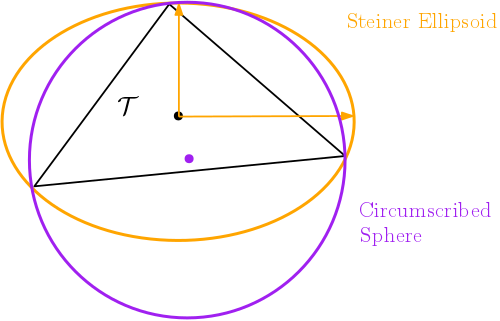
\includegraphics[scale=0.4]{ellipsoid_and_sphere}
	\caption{A simplex $\ssplx\subset\R^2$ and  its corresponding Steiner circumscribed ellipsoid in orange (light) and circumscribed sphere in purple (dark). The arrows illustrate the semi-axes of the ellipsoid.}
	\label{fig:ellipsoid_and_sphere}
\end{figure}

The appearance of the  eigenvalues  in  the semi-axes allows us to relate the volumes of $\El(\splx_G)$ and $\El(\splx_G^+)$.  The volume of an  ellipsoid in $\R^{n-1}$ written in the standard  form mentioned  above is 
\begin{equation*}
\frac{\pi^{\frac{n-1}{2}}}{\Gamma(\frac{n+1}{2})} \det(\bS^{-1}),
\end{equation*}
where $\Gamma(z)$ is the gamma function.  We emphasize  that the gamma function is distinct from $\Gamma_G$, the  total weight of spanning trees in $G$.  
For $\El(\splx_G)$, $\bS = \sqrt{\frac{n}{n-1}} \Eval^{-1/2}$, so 
\begin{align*}
\vol(\El(\splx_G)) &= \frac{\pi^{\frac{n-1}{2}}}{\Gamma(\frac{n+1}{2})} \bigg(\frac{n-1}{n}\bigg)^{\frac{n-1}{2}} \det\Eval^{1/2} \\
&= \frac{\pi^{\frac{n-1}{2}}}{\Gamma(\frac{n+1}{2})} \bigg(\frac{n-1}{n}\bigg)^{\frac{n-1}{2}}\bigg(\prod_{i<n}\lambda_i\bigg)^{1/2} \\
&= \frac{\pi^{\frac{n-1}{2}}}{\Gamma(\frac{n+1}{2})} \bigg(\frac{n-1}{n}\bigg)^{\frac{n-1}{2}} \sqrt{n}\Gamma_G^{1/2}.
\end{align*}

Moreover, as was noticed by Devriendt  and  Van Mieghem~\cite{devriendt2018simplex},  the linear dependence of both $\vol(\El(\splx_G)$ and $\vol(\splx_G)$ on $\Gamma_G^{1/2}$ (recall Corollary~\ref{cor:vol(SG)}) implies their ratio is independent of the particular graph $G$: 
\begin{equation*}
\frac{\vol(\El(\splx_G))}{\vol(\splx_G)} = \frac{\pi^{\frac{n-1}{2}}}{\Gamma(\frac{n+1}{2})} \bigg(\frac{n-1}{n}\bigg)^{\frac{n-1}{2}} \frac{(n-1)!}{\sqrt{n}}.
\end{equation*}

A similar procedure may be performed  with $\vol(\El(\splx_G^+))$  and $\vol(\splx_G^+)$. In that  case we  have 
\begin{align*}
\vol(\El(\splx_G^+)) = \frac{\pi^{\frac{n-1}{2}}}{\Gamma(\frac{n+1}{2})} \bigg(\frac{n-1}{n}\bigg)^{\frac{n-1}{2}} \det\Eval^{-1/2} = \frac{\pi^{\frac{n-1}{2}}}{\Gamma(\frac{n+1}{2})} \bigg(\frac{n-1}{n}\bigg)^{\frac{n-1}{2}} (n\Gamma_G)^{-1/2}.
\end{align*}
The ratio  of $\vol(\El(\splx_G^+))$ to $\vol(\splx^+_G)$ is the same as above. 



Next we investigate the circumscribed sphere of the combinatorial  simplex. Similarly to the circumscribed ellipsoid, the \emph{cirscumscribed sphere  of a convex body $\P$} is the sphere whose boundary contains all the vertices of $\P$. The circumscribed sphere does not exist in general. However, just as it is possible to always draw a circle containing the endpoints  of a triangle, so the circumscribed sphere of a hyperacute simplex always exists  as is demonstrated  by the following lemma.  

\begin{lemma}[\cite{fiedler1993geometric}]
	\label{lem:circ_sphere}
	Let $\splx^+\subset\R^{n-1}$ be a hyperacute simplex. The circumscribed sphere  of $\splx^+$ exists and is given by the set of points $\{\x:\x=\Sv\balpha, \; \la \balpha,\one \ra = 1, \; \la \balpha,\D\balpha\ra =0\}$, which is a sphere centred at the point $\frac{1}{2}\Sv(\L_G\bD + \one/n)$ with radius $\frac{1}{2}\sqrt{\bD^\tp\L_G\bD + 4\Rtot_G/n^2}$ where $G$ is $\splx^+$'s associated graph, and $\bD = \diag(\L_G^+(i,i))$. 
\end{lemma}

\begin{remark}
	It is no coincidence that the radius of the sphere is related to the top left entry in the  inverse of the Menger matrix  associated with  $\splx^+$. This was  noticed by Fiedler and is relied  upon in  the proof of Lemma~\ref{lem:circ_sphere}. 
\end{remark}


Until this point, we have been examining only the quadrics associated with the combinatorial simplices. We now consider the normalized simplices. Since all the vertices of the normalized simplex lie on the unit sphere, it's clear  that the circumscribed sphere of $\splxn_G$ is precisely $\{\x:\x^\tp\x=1\}$. It's not as straightforward  to see what they circumscribed ellipsoid, $\El(\splxn)$, is on the other hand. One might suspect that it obeys the  equation $\x^\tp \Svn^+(\Svn^+)^\tp=1-1/n$, as this is the natural analogue of \eqref{eq:steinerE}. However, because $\Svn^+$ and $\Svn$ obey a non-constant pseudoinverse relation, this equation fails the first test: $\svn_i^\tp\Svn^+(\Svn^+)^\tp\svn_i = \bchi_i^\tp(\I-\sqrt{\w}\sqrt{\w}^\tp/\vol(G))\bchi_i=1-\sqrt{w(i)w(j)}/\vol(G)$ is not constant. 
However, at this point we recall that beyond being simply  the inverse simplex of $\splx$, $\splx^+$ is also its dual.  We might thus hazard a guess that the correct matrix is $\Svn^\du (\Svn^\du)^\tp$, where $\Svn^\du$ is the vertex matrix of $\splxn^\du$. The  following lemma  confirms this hypothesis and, moreover, verifies that similar reasoning can be applied to the Steiner Ellipsoid of any simplex---not only those corresponding to graphs.  

\begin{lemma}
	\label{lem:El(T)_general}
	Let $\ssplx\subset\R^{n-1}$ be a simplex whose dual has vertex matrix  $\Sv^\du$. Then  the Steiner ellipsoid of $\ssplx$ is 
	\begin{equation*}
	\El(\ssplx) = \bigg\{\x:\x^\tp\Sv^\du(\Sv^\du)^\tp\x=\frac{n-1}{n}\bigg\}.
	\end{equation*} 
\end{lemma}

\begin{proof}
	The computation is almost identical to that in the proof of Lemma~\ref{lem:El(S)}, except we  take $\M=\Sv^\du(\Sv^\du)^\tp$ and use the general relationship between  $\Sv^\tp\Sv$ and $\Sv^\du(\Sv^\du)^\tp$ given by Lemma~\ref{lem:dual_pseudoinverse}. 
\end{proof}


\section{Resistive Polytope}
\label{sec:resistive_polytope}
In this section we explore the relationship between the inverse combinatorial simplex of $G$ and another geometric object related to the effective resistance of the graph. Consider the vertices $\bmu_i=\L_G^{+/2}\bchi_i\in\R^n$, for $i\in[n]$. This yields $n$ points in $\R^n$, also with pairwise squared distances equal to the effective resistance of the graph: 

\begin{equation*}
\norm{\bmu_i-\bmu_j}_2^2 = \norm{\L_G^{+/2}(\bchi_i-\bchi_j)}_2^2 =  (\bchi_i-\bchi_j)^\tp \L_G^+(\bchi_i-\bchi_j)=\effr(i,j).
\end{equation*}

This embedding has been referred to as a \emph{resistive embedding}~\cite{shayanNotes,ding2011cover}, and is an example of an $\ell_2^2$ metric~\cite{arora2009expander} owing  to the well known fact that the effective resistance is a metric (e.g., ~\cite{klein1993resistance}). That being said however, while the mapping seems to be known~\cite{ghosh2008minimizing}, there is very little literature on its properties. 

Set 
\begin{equation}
\label{eq:res_pol}
\respol_G \equiv \conv(\{\bmu_i\}),
\end{equation}
and  call  $\respol_G$ the \emph{resistive polytope of $G$}. Note that $\L_G^{+/2}$ is $\respol_G$'s vertex matrix. As usual, we may omit the subscript $G$ for convenience. We emphasize that while the vertices $\{\bmu_i\}$ obey the same pairwise  distances as  those of the inverse simplex $\splx_G^+$, $\respol_G$  is not the same object as $\splx_G^+$. First, of course, there is  the fact that it sits in  $\R^n$. However,  we also note that the entries of $\mu_i$ (the first $n-1$, at least) do not match those of $\sv_i^+$. Indeed, 

\begin{align*}
\mu_i(\ell) = \L_G^{+/2}(\ell,i) = \sum_{j\in[n]}\lambda_j^{-1/2}\vp_j\vp_j^\tp(\ell,i) = \sum_{j\in[n]}\lambda_j^{-1/2}\vp_j(\ell)\vp_j(i).
\end{align*}
Recalling the formula for the vertices of the inverse simplex $\splx^+$ demonstrates that 
\begin{equation*}
\mu_i(\ell) = \sum_{j\in[n]}\sv_\ell^+(j)\vp_j(i) = \sum_{j\in[n]}\sv_i^+(j)\vp_j(\ell).
\end{equation*}
Hence, in general, $\mu_i(\ell)\neq \sv_i^+(\ell)$. However, the dot product between the vertices of $\respol_G$ does respect  the same relationships as those between the vertices of $\splx_G^+$:
\begin{align*}
\la \bmu_i,\bmu_j\ra &=\sum_{\ell\in[n]} \L_G^{+/2}(\ell,i)\L_G^{+/2}(\ell,j) \\
&= \la \L_G^{+/2}(\cdot,i),\L_G^{+/2}(\cdot,j)\ra \\
&=\la \L_G^{+/2}(\cdot,i),\L_G^{+/2}(j,\cdot)\ra= \L_G^+(i,j),
\end{align*}
since $\L_G^{+/2}$ is symmetric and  $\L_G^{+/2}\L_G^{+/2}=\L_G^+$.  We can also see this from recalling that 
\[\effr(i,j) = \L_G^+(i,i) + \L_G^+(j,j) - \frac{1}{2}\L_G^+(i,j),\]
combined with the facts that $\norm{\bmu_i-\bmu_j}_2^2 = \effr(i,j)$ and $\norm{\bmu_i}_2^2 = \L_G^+(i,i)$. The centroid of $\re_G$ also coincides with the origin  of $\R^n$: 
\begin{equation*}
\cent(\re_G) = \frac{1}{n}\L_G^{+/2}\one = \frac{1}{n}\sum_{i\in[n-1]}\lambda_i^{-1/2}\vp_i\vp_i^\tp \one = \zero.
\end{equation*}

One therefore begins to suspect that $\respol_G$ is the same object of  $\splx_G^+$, simply projected onto some hyperplane of $\R^n$. The following lemma  demonstrates that this is indeed the  case, and  that  the hyperplane  is that which is has $\spn(\one)$ as its orthogonal complement. See Figure~\ref{fig:res_embedding} for an  illustration. 

\begin{lemma}
	The all ones vector is orthogonal to $\re_G$. 
\end{lemma}
\begin{proof}
	We need to show that for all $\p,\q\in\re_G$, $\la \one,\p-\q\ra=0$. As usual, let $\x$ and $\y$ be the barycentric coordinates of $\p$ and $\q$ so that $\p=\L_G^{+/2}\x$ and $\q=\L_G^{+/2}\y$. We have
	\begin{align*}
	\la \one,\p\ra &= \sum_{\ell\in[n]} (\L_G^{+/2}\x)(\ell) = \sum_{\ell\in[n]} \sum_{j\in [n]}\L_G^{+/2}(\ell,j)x(j) = \sum_{j\in[n]}x(j) \sum_{\ell\in[n]}\L_G^{+/2}(\ell,j),
	\end{align*}
	where for any $j$, 
	\[\sum_{\ell\in[n]}\L_G^{+/2}(\ell,j)= \one^\tp \L_G^{+/2}\bchi_j=\sum_{\ell\in[n-1]} \lambda_\ell^{-1/2}\one^\tp \vp_\ell\vp_\ell^\tp\bchi_j=0,\]
	since $\vp_i\in\spn(\one)^\perp$  for all $i<n$. Hence  $\la \one,\p\ra=0$ meaning that $\la \one,\p-\q\ra=0$ as well. 
\end{proof}

\begin{figure}
	\centering
	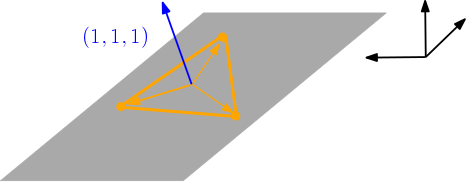
\includegraphics[scale=0.5]{res_embedding}
	\caption{The resistive embedding (in orange;  light) of a graph with three nodes sits in a plane (gray) which is parallel to the all ones vector. }
	\label{fig:res_embedding}
\end{figure}

The relationship between $\re$ and $\splx$ gives us an alternate way to prove equalities such as \eqref{eq:c(S_U)}: There exists an isometry\footnote{A distance preserving map.} between $\re$ and $\splx$, so 
\begin{equation*}
\norm{\cent(\splx^+_U)}_2^2 = \norm{\cent(\re_U)}_2^2 = \frac{1}{|U|^2} \norm{\L_G^{+/2}\bchi_U}_2^2 = \frac{1}{|U|^2}w(\delta^+ U).
\end{equation*}


Additionally, just as $\splx_G^+$  has  the inverse $\splx_G$, $\respol_G$  has an inverse which respects the same  relationships. As one might guess, this inverse has vertex matrix $\L_G^{1/2}$. To see this, for any $i,j\neq k$,  we have 
\begin{equation*}
\la \L_G^{1/2}\bchi_i,\L_G^{+/2}\bchi_j-\L_G^{+/2}\bchi_k\ra = \bchi^\tp \L_G^{1/2}\L_G^{+/2}(\bchi_j-\bchi_k)\ra,
\end{equation*}
where 
\begin{align*}
\L_G^{1/2}\L_G^{+/2} &= \sum_{r,s=1}^{n-1}\lambda_r^{1/2}\lambda_s^{-1/2}\vp_r\vp_r^\tp\vp_s\vp_s^\tp = \sum_{r=1}^{n-1} \vp_r\vp_r^\tp,
\end{align*}
and 
\begin{align*}
\sum_{r=1}^{n-1}\bchi_i \vp_r\vp_r^\tp\bchi_j = \sum_{r=1}^{n-1}\vp_r(i)\vp_r(j) = \delta_{ij} - \frac{1}{n},
\end{align*}
using Equation \eqref{eq:sum_double_ortho}. Hence, 
\begin{align*}
\bchi_i^\tp \L_G^{1/2}\L_G^{+/2}(\bchi_j-\bchi_k) = \delta_{ij} - \frac{1}{n} - (\delta_{ik}-\frac{1}{n}) = \delta_{ij}.
\end{align*}

To  conclude, there exists an isometry between the inverse combinatorial  simplex of a graph $G$ (which  lies in $\R^{n-1}$) and the effective  polytope, $\re_G$ of  $G$ (which  lies in $\R^n$). The resistive polytope lies in a hyperplane orthogonal to the  all-ones vector.  



%\section{Effective  Resistance  \&  Dynamics}
%\label{sec:dynamics}
%In this section we briefly highlight a few connections between stochastic process on $G$ and  the geometry of its inverse combinatorial simplex $\splx_G^+$. 



\section{Continuous Time Random Walks}
\label{sec:random_walks}
This current section is for the reader who is less interested  in the  mathematics  behind the graph-simplex correspondence, and is reading only for the vague  hope  that some of the underlying geometry will be aesthetically pleasing. While  the  content has certainly failed in this vein thus far, this section  is the closest we will come to remedying the situation. 

Consider a  random walk on a graph. The probability distribution  governing the dynamics is a barycentric  coordinate: each coordinate is non-negative and they sum to one. Therefore, we can represent the probability distribution as a point in the simplex and the probability  distribution as a function of time as a path in the simplex. See Figure~\ref{fig:random_walk} for an illustration. In what follows we give equations which determine the dynamics of the path in the simplex as a function of the eigenvalues  and eigenvectors  of the graph. 

We will examine a continuous time random walk which  obeys the equation 
\begin{equation*}
\frac{d \bpi(t)}{dt } = -\L_G\W_G^{-1/2} \bpi(t),
\end{equation*}
and has the solution $\bpi(t)  = \exp(-\L_G\W_G^{-1/2}t)\bpi(0)$. This, however, is relatively unsightful in terms of  analyzing the dynamics of $\bpi(t)$ in terms of the  graph.  Instead, in  what follows we seek  to develop a solution to $\bpi(t)$ in terms of the  eigendecomposition of  $G$.  Define $\bpi_1(t) = \W^{-1/2}\bpi(t)$ and $\bpi_2(t) = \Eign^\tp \bpi_1(t)$, where we recall that $\Eign^\tp$ is the eigenvector matrix  of  $\Ln_G$.  Then 
\begin{equation*}
\frac{d \bpi_1(t)}{dt} = \W^{-1/2}\frac{d \bpi(t)}{dt} = -\W^{-1/2}\L_G\W^{-1/2}\W^{-1/2}\bpi(t) = - \Ln_G\bpi_1(t),
\end{equation*}
and, using the eigendecomposition of $\Ln_G$,   
\begin{equation*}
\frac{ d\bpi_2(t)}{dt} = \Eign^\tp \frac{d\bpi_1(t)}{dt} = -\Eign^\tp \Ln_G \bpi_1(t) = -\Eign^\tp \Eign\Evaln\Eign^\tp \bpi_1(t) = -\Evaln  \bpi_2(t),
\end{equation*}
since  $\Eign^\tp\Eign=\I$. This equation  has the solution 
\begin{equation*}
\bpi_2(t) = \exp(-\Evaln t)\bpi_2(0) = \begin{pmatrix}
e^{-\lambda_1 t}  & &\\
& \ddots  & \\
&& e^{-\lambda_{n-1} t}
\end{pmatrix}  \bpi_2(0).
\end{equation*}

\begin{figure}
	\centering
	\begin{minipage}{0.32\textwidth}
		\centering
		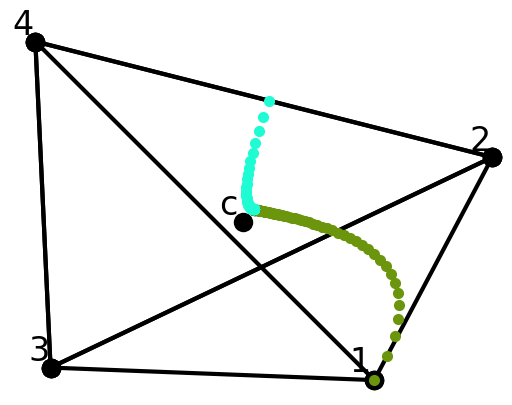
\includegraphics[scale=0.6]{dynamics1}
		\subcaption{}
	\end{minipage}
	\begin{minipage}{0.32\textwidth}
		\centering
		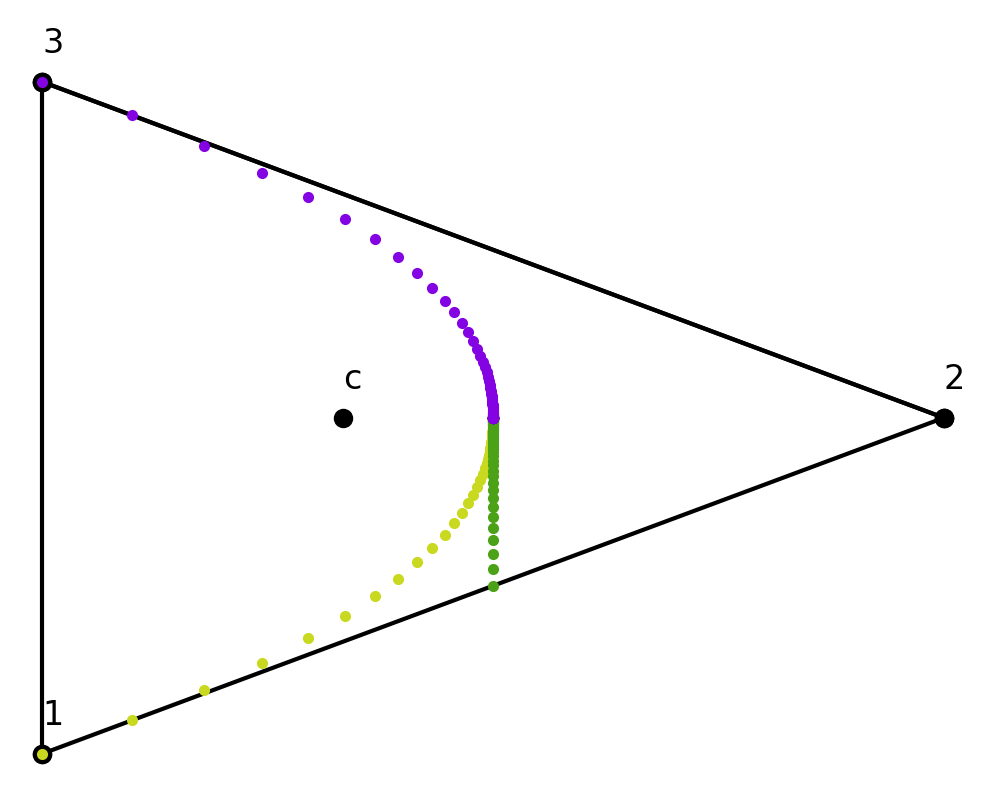
\includegraphics[scale=0.4]{dynamics3}
		\subcaption{}
	\end{minipage}
	\begin{minipage}{0.32\textwidth}
		\centering
		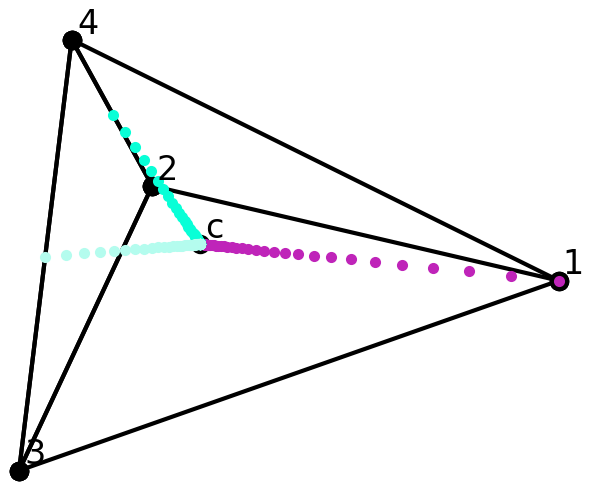
\includegraphics[scale=0.6]{dynamics2}
		\subcaption{}
	\end{minipage}
	\caption{Random walk dynamics plotted as points  in the simplex. Figures (a) and (b) are plotted using the normalized simplex;  figure (c) uses  the normalized simplex. The  underlying graph of Figure (a) has edges $(1,2)$, $(2,3)$, $(3,4)$, $(2,4)$, that underlying (b) edges $(1,2)$ and $(2,3)$ and that of (c) is the complete graph  $K_4$. }
	\label{fig:random_walk}
\end{figure}

Combining the  definitions of $\bpi_1$  and $\bpi_2$ gives $\bpi_2(t)  = \Eign^\tp \bpi_1(t) = \Eign^\tp \W^{-1/2}\bpi(t)$, hence 
$\bpi(t) = \W^{1/2} \Eign \bpi_2(t)$. As a point in the  simplex this gives 
\begin{equation*}
\p(t)  = \Sv\bpi(t) = \Eval^{1/2}\Eig^\tp \W^{1/2}\Eign \bpi_2(t) = \Y\bpi_2(t),
\end{equation*}
after defining $\Y\equiv \Eval^{1/2}\Eig^\tp \W^{1/2}\Eign$. As a point in the normalized simplex, we have 
\begin{equation*}
\q(t) = \Svn\bpi(t) = \Evaln^{1/2}\Eign^\tp\W^{1/2}\Eign\bpi_2(t) = \Yn\bpi_2(t),
\end{equation*}
where $\Yn= \Evaln^{1/2}\Eign^\tp\W^{1/2}\Eign$. We thus  see that the matrices 
\begin{equation*}
\Y = \begin{pmatrix}
\lambda_1^{1/2}\sum_{i\in[n]} \vp_1(i)\vpn_1(i) w_i^{1/2} & \dots &  \lambda_1^{1/2}\sum_{i\in[n]} \vp_1(i)\vpn_{n-1}(i) w_i^{1/2} \\
\vdots & \ddots & \vdots \\
\lambda_{n-1}^{1/2}\sum_{i\in[n]} \vp_{n-1}(i)\vpn_1(i) w_i^{1/2} & \dots &  \lambda_{n-1}^{1/2}\sum_{i\in[n]} \vp_{n-1}(i)\vpn_{n-1}(i) w_i^{1/2} 
\end{pmatrix},
\end{equation*}
and  
\begin{equation*}
\Yn  = \begin{pmatrix}
\lambdan_1^{1/2}\sum_{i\in[n]} \vpn_1(i)\vpn_1(i) w_i^{1/2} & \dots &  \lambdan_1^{1/2}\sum_{i\in[n]} \vpn_1(i)\vpn_{n-1}(i) w_i^{1/2} \\
\vdots & \ddots & \vdots \\
\lambdan_{n-1}^{1/2}\sum_{i\in[n]} \vpn_{n-1}(i)\vpn_1(i) w_i^{1/2} & \dots &  \lambdan_{n-1}^{1/2}\sum_{i\in[n]} \vpn_{n-1}(i)\vpn_{n-1}(i) w_i^{1/2} 
\end{pmatrix},
\end{equation*}
govern the dynamics of the random walk in  $\splx_G$ and $\splxn_G$, respectively.  More specifically, letting $\Y=(\y_1\;\dots\;\y_n)$ we have 
\[\p(t) = \sum_{i\in[n-1]} \y_i (\bpi_2(t))(i) = \sum_{i\in[n-1]}  \y_i e^{-\lambda_i t} \Eign^\tp \W^{-1/2}\bpi(0)(i),\]
and a similar  equation for $\q(t)$. 







\chapter{Algorithmics}
\label{chap:algorithmics}

\chapterquote{I'm smart enough to know that I'm dumb. }{Richard Feynman}

\chapterquote{Beware of bugs in the above code; I have only\\ proved it correct, not tried it.}{Donald  Knuth}

This final technical chapter will discuss some of the algorithmic foundations and consequences of the graph-simplex correspondence. Vis-\`{a}-vis foundations, we will chiefly be concerned with transitioning between a graph and its various simplices. We will explore lower bounds for how quickly this can be done if we wish to obtain the precise result\footnote{Ignoring issues of floating point number accuracy}, and whether we can ``approximate'' any of the constructions (e.g., given the graph $G$ can we quickly obtain a simplex which serves as an approximation\footnote{The notion of approximating a simplex is rather ambiguous and will be expounded upon at a later time.} to $\splx_G$.) With respect to algorithmic consequences on the other hand, we will attempt to leverage knowledge we have in the hitherto relatively unrelated areas of computational graph theory and high-dimensional computational geometry to draw new conclusions about the complexity of several problems in these areas. For instance, if a  graph theoretic problem has an analogue in the simplex, any fact regarding the problem's difficulty---whether it's NP-complete, say---translates to an immediate result about its geometric counterpart. In particular, since the simplex of a graph can be generated in polynomial time given the graph (due to the fact that an eigendecomposition can be computed in polynomial time) and vice versa, problems which are solvable in polynomial time in either the simplex or graph domain  translate to polynomially solvable (yet perhaps not optimal!) problems in the other domain and likewise, problems which are \NP-hard in one domain have analogues which are \NP-hard in the other. 

For the benefit of the reader unfamiliar with computational complexity and reductions, we begin the chapter with a short section containing this background material. We will also discuss computational representations of a simplex therein. 

\section{Preliminaries}
\label{sec:algorithmics_prelims}
\paragraph{Asymptotics.}
We begin with asymptotic notation which will be used to analyze the running time of various algorithms. We use the standard definitions---see any reference text on algorithm design for more background (e.g., \cite{kleinberg2006algorithm}). Let $f,g:U\subset \R \to \R$ be functions. Write $f=O(g)$ (or $f(n)=O(g(n))$) if $\limsup_{x\to \infty}|f(x)/g(x)|<\infty$, and $f=\Omega(g)$ if $g=O(f)$. Write $f=o(g)$ as $x\to c$ if $\lim_{x\to \infty}|f(x)/g(x)|=0$ and $f=\omega(g)$ if $g=o(f)$. If $f=O(g)$ and $f=\Omega(g)$ we write $f=\Theta(g)$. We will also use the tilde to hide polylog factors. Say $f=\tO(g)$ if $f(n) = O(g(n) \log^c n)$ and $f=\tOmega(g)$ if $f(n) = \Omega(g(n) \log^{-c}n)$, for some $c\geq 0$. 


\paragraph{Simplex representations.}
In order to discuss the algorithmics pertaining to simplices and convex polyhedra in general, we must discuss how such objects are represented by a machine. Clearly, we cannot simply enumerate all the points enclosed by a body in high-dimensional space. Instead we must concisely represent the boundaries of the polytope. The two most common such descriptions are 
\begin{itemize}
	\item \textsf{V}-\emph{description}, in which we are given the vertex vectors of the polytope; 
	\item \textsf{H}-\emph{description}, in which we are given the parameters of the half-spaces whose intersection defines the polytope. That is, if $\ssplx=\bigcap_i \{\x:\la \z_i,\x\ra \geq b_i\}$, then an \hdesc of $\ssplx$ would be the vectors $\{\z_i\}$ and the scalars $\{b_i\}$. 
\end{itemize}

It's not at all clear whether these descriptions are equivalent in the sense that one can easily generate one from the other. Indeed, the complexity of vertex enumeration (generating a \vdesc from an \hdesc) and facet enumeration (generating an \hdesc from a \vdesc) remains an open problem for general polytopes~\cite{kaibel2003some}, although there exist polynomial time algorithms when the polytopes are simplices (e.g., \cite{bremner1998primal}). We will return to this fact later on. 

We end by remarking that when discussing general  polytopes, we continue  to work  in $\R^{n-1}$ as a vector space. Thus,  the vertices of the polytope are still vectors which begin at the origin. 

\paragraph{Reductions.}
Some background on computational models and reductions will also be useful. For more details see~\cite{kleinberg2006algorithm} or \cite{knuth2011art}. We will use the typical computational model for analyzing algorithms. Without diving too far into the minutiae, we assume that single arithmetic operations require $O(1)$-time, i.e., constant. We will analyze the runtime of an algorithm as a function of how many bits it takes to represent the input. A common tool for providing upper bounds on the runtime of an algorithm is to ``reduce'' it to a problem for which a bound is already known. Assume problem $P$ requires time $\Omega(f_P(n))$ to solve---meaning that \emph{any} algorithm requires time $\Omega(f_P(n))$---where $n$ represents the size of the input and $f_P(n)$  is some function of $n$, e.g., $f_P(n) =  n^2\log n$. Let $Q$ be a distinct problem and suppose that for every instance of $P$ we can transform the input of $P$ to a valid input for $Q$, and transform the output of $Q$ to a valid output of $P$, both in time $O(f_P(n))$.  We have then established that $f_Q(n) = \Omega(f_P(n))$, where $f_Q$ the runtime required to solve $Q$, since we can solve $P$ in time $f_Q(n) + O(f_P(n))$ by transforming any input to $P$ to the input of $Q$, solving $Q$, and transforming the output back. Such a technique will be used extensively throughout the next few sections. 

\paragraph{The complexity classes \NP, \NP-hard, and \NP-Complete.}
For brevity, we restrict ourselves to a very brief presentation of these concepts. The interested reader can find more background in any reference  on computational  complexity theory. 

The class \NP  is  the set of all decision problems\footnote{That is,  problems  to which we seek a yes/no answer.} which have solutions which are \emph{verifiable} in polynomial time. It is possible, for example, to check  in polynomial time whether  a given  set is in fact an independent set of a certain size. Thus the decision variant of \iset lies in \NP. \NP stands for ``non-deterministic polynomial time'', as it is formally the set of all  decision problems solvable by a non-deterministic Turing  Machine~\cite{papadimitriou2003computational}. 

The class \NP-hard comprises all the problems to  which  any problem in \NP can be reduced in polynomial time (see above). That is, $P\in\NP$-hard iff for all  $Q\in\NP$,  $Q$ can be  reduced to $P$ in polynomial time. Thus,  to show that $P\in\NP$-hard, it suffices to reduce another problem $R\in\NP$-hard to  $P$ (in polynomial time) since,  in this  case, if all problems in \NP are  reducible  to  $R$  they are in turn  reducible  to  $P$. We  tend to think of \NP as the set of ``hard'' problems. 

Finally,  the class \NP-complete is the intersection of the classes \NP and  \NP-hard. Informally then, it is  the  class of all ``hard'' decision problems. 

\begin{figure}
	\centering
	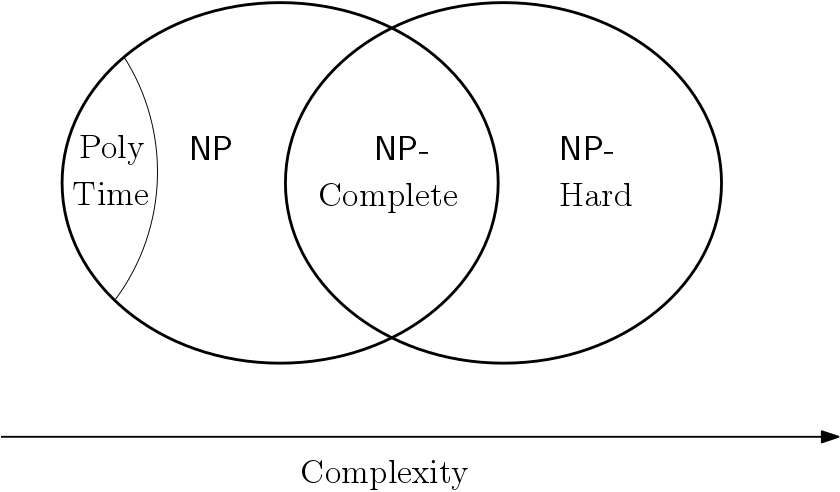
\includegraphics[scale=0.28]{NP_diagram}
	\caption{Illustration of the relationships between the  classes \NP,  \NP-hard, and \NP-complete. ``Poly-time'' refers to problems with polynomial time solutions. Such algorithms can trivially be verified  in polynomial time, hence  are a  subset of problems in \NP. We emphasize that the diagram is  for intuitive purposes only,  and may not reflect the true relationships between these classes. For example, in  the unlikely  case that \textsf{P}=\NP (i.e., all problems in  \NP are solvable in polynomail time), then the regions ``Poly time'', \NP and \NP-complete coincide.}
\end{figure}



\section{Computational Complexity}
\label{sec:algorithmics_complexity}

In this section we investigate the relationships between problems in one domain---either the graph-theoretic or geometric domain---and their analogues in the other. The following result exemplifies the power of the graph-simplex correspondence in yielding results which seem otherwise difficult to obtain (certainly more difficult than the following proof, at any rate).  
It was first stated by Devriendt and Van Mieghem~\cite{devriendt2018simplex} for inverse combinatorial  simplices, and can be slightly generalized as follows.  

\begin{lemma}
	\label{lem:altitude_hard}
	Computing the altitude of minimum length in any simplex is \NP-hard. 
\end{lemma}
\begin{proof}
	The relationship $\norm{\alt(\splx^+_U)}_2^2 = w(\partial U)^{-1}$ (Lemma \ref{lem:alt}) for the inverse simplex of a graph $G$ demonstrates that the problem of computing a minimum length altitude in any hyperacute simplex is \NP-hard, because computing the  maximum weight cut in any weighted graph is \NP-hard~\cite{karp1972reducibility}.  Since the  class  of all hyperacute simplices is contained in the class of all simplices, the result follows.  
\end{proof}

\begin{remark} In  the above statement and its proof, the description of the polytope and simplex was not specified. This is due to the fact that---as discussed above---for simplices there is a polynomial time algorithm to translate betweent the various descriptions. With regard to \NP-completeness therefore, the description makes no difference. Consequently, we will continue to ignore this distinction for the remainder of this section. 
\end{remark}


\begin{remark}
Altitudes do  not have  an analogue in general polyhedra. However, for  those problems which do have analogues, 
if they are \NP-hard for hyperacute simplices then are so for general polyhedra (since simplices are a subclass of polyhedra). Henceforth, we might use this observation  without justification. 
\end{remark}


The remainder of this section is dedicated to obtaining more results of this type. 

We begin by investigating independent sets. Given a graph $G=(V,E,w)$, recall that an \emph{independent set} is a subset $I\subset V$ such that if $i,j\in I$ then $(i,j)\notin E$. 
The weight of an independent set is nicely described by the Laplacian quadratic form. If $I$ is an independent set note that 
\[\vol(I) = w(\partial I),\] 
and so 
\begin{align*}
    \Lf(\bchi_I) = \sum_{i\sim j}w(i,j)(\bchi_I(i)-\bchi_I(j))^2 = \sum_{i\in I}\sum_{j:j\sim i} w(i,j) = \sum_{i\in I}w(i)=w(\partial I),
\end{align*}
where the second and fourth inequalities follows from the fact that $I$ is an independent set. Now, suppose we assign each vertex $i$ a weight $f(i)\geq 0$. The \mwis problem consists of maximizing $f(I)\equiv \sum_{i\in I}f(i)$ over all independent sets $I$. Clearly \mwis is \NP-hard in general, seeing as it reduces to the usual independent set maximization problem by taking $f(i)=1$ for all $i$. If $f$ is a linear function of the weights so that $f(i)=\alpha w(i)$ for all $i$ and some $\alpha> 0$, we call the corresponding problem $\alpha$-\vwis. We will focus on the case $\alpha=1$ for clarity, and call the  corresponding problem just \vwis. The difficulty of this problem is not immediately clear, since it is more structured than simply \mwis. The next lemma removes any doubt as to the problem's tractability.   

\begin{figure}
	\centering
	\begin{minipage}{0.3\textwidth}
		\centering
		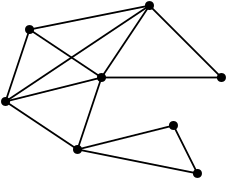
\includegraphics[scale=0.4]{graph}
		\subcaption{}
	\end{minipage}
	\begin{minipage}{0.3\textwidth}
		\centering
		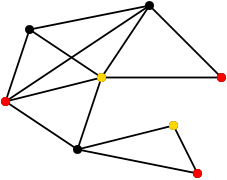
\includegraphics[scale=0.4]{independent_sets}
		\subcaption{}
	\end{minipage}
	\begin{minipage}{0.3\textwidth}
		\centering
		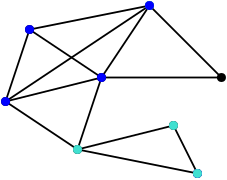
\includegraphics[scale=0.4]{cliques}
		\subcaption{}
	\end{minipage}
	\caption{(a) A connected  graph. (b) Two of its independent sets; one in red (dark) and one yellow (light). The red set constitutes a maximum sized independent set. (c) Two of its cliques; one in blue (dark), one  turquoise (light). The blue  set constitutes a maximum sized clique.}
	\label{fig:is+cliques}
\end{figure}

\begin{lemma}
	\label{lem:vwis}
	\vwis is \NP-Complete. 
\end{lemma}
\begin{proof}
	Given a purported independent $I$, it is easily checkable in polynomial time whether $\vol(I)$ is of a certain size---hence \vwis is in \NP. 
	To that it is \NP-hard, we reduce from \iset. Let $G=(V(G),E(G))$ and  $k\in\N$ be an instance of \iset. The intuition behind the following reduction is to create a separate graph $H$ which, for each independent set $I\subset V(G)$, has an independent set $J$ in $H$ such that  $\vol_H(J)=|I|$ in $H$ and conversely, for each maximal independent set $J$ in $H$ there exists an independent set $I$ in $G$ with $|I| = \vol_H(J)$. From this relationship it follows that $G,k$ constitutes a yes instance to \iset iff $H,k$ is a yes instance to \mwis.  After wordsmithing the intuition, let us proceed to the formal argument. 

	Construct a graph $H=(V(H), E(H))$ as follows. For each vertex $u\in V(G)$, create $\deg_G(u)+1$ vertices $u_0,u_1,\dots,u_{\deg_G(u)}$ in $V(H)$. For $1\leq k\leq \deg_G(u)$ set \[w_H(u_k) =  \frac{1}{\deg_G(u)}.\] Construct the edge set $E(H)$ such that the neighbours of each vertex are described by 
	\begin{equation*}
	\partial_{H}(u_k) = \{u_0\}\cup \bigcup_{v\in \partial_G(u)}\{v_\ell: 0\leq \ell\leq \deg_G(v) \}.
 	\end{equation*}
	In words, $u_k$ is connected to all the vertices representing $v$ if $(u,v)\in E(G)$, and to $u_0$. Now, let $I\subset V(G)$ be an independent set in $G$ and consider the set
	\[J = \{v_k: v\in I, 1\leq k\leq \deg_G(v)\}.\]
	We claim that $J$ is an independent set in $H$. 
	Indeed, if $v_k,u_\ell\in J$ and  $(v_k,u_\ell) \in E(H)$ for some $k\in[\deg_G(v)]$, $\ell\in[\deg_G(u)]$ then $v\in d_G(u)$ by definition of $\partial_H(u)$. Since $I$ is an independent set however, both $u$ and $v$ are not in $I$, a contradiction. This demonstrates that $J$ is bonafide independent set. Moreover, 
	\[\vol_H(J) = \sum_{v\in I}\sum_{k=1}^{\deg_G(u)} w_H(v_k) = \sum_{v\in I}\sum_{k=1}^{\deg_G(u)} \frac{1}{\deg_G(u)} = |I|.\]

	Conversely, let $J$ be an independent set in $H$. We claim that there exists an independent $J'$ in $H$ with $\vol_H(J')\geq \vol_H(J)$ containing only vertices of the form $v_\ell$ for $\ell\geq 1$, i.e., not $v_0$. Initially, set $J'=J$ but suppose $v_0\in J$. Replace $v_0$ by $v_1,\dots,v_{\deg_G(v)}$ in $J'$.  None of the these vertices share edges, and aside from one another, $v_\ell$ and $v_0$ for $\ell>0$ have the same edge set. It follows that $J'$ remains an independent set. Moreover, since $w_H(v_0) < w_H(v_\ell)$ by construction, we have $\vol_H(J)< \vol_H(J')$. Let us remark further that if $J$ contains vertices $\{v_\ell\}_{\ell\in F}$ for some $F\subsetneq  [\deg_G(v)]$, then we may add the missing vertices $v_k$, $k\in [\deg_G(v)]\setminus F$ while maintaining the property that $J$ is an independent set (this follows since $\partial_H(v_k) = \partial_H(v_\ell)$ for all  $\ell,k\geq1$). We have thus argued that every maximal independent set in $H$ can be written in the form $J= \cup_{v\in I}\{v_k: 1\leq k\leq \deg_G(v)\}$ for some set $I\subset V(G)$. We now claim that $I$ is an independent set in $G$. The argument is similar to above: If not, then $u,v\in I$ with $u\sim v$, but this implies that $v_k\sim v_\ell$ in $H$ meaning that $J$ is not an independent set.  Additionally, as above, $\vol_H(J)=|I|$. Therefore, there exists an independent set $J$ in $H$ with $\vol_H(J)\geq k$ iff there exists an independent set $I$ in $G$ with $|I|\geq k$, concluding the argument. 
\end{proof}

This result allows us to conclude that certain optimizations problems in hyperacute simplices---thus convex polytopes in general---are \NP-hard. 

\begin{lemma}
	Let $\P$ be a convex polytope with vertex set $V$. The optimization problem 
	\begin{alignat*}{2}
	\min_{I\subset V, I\neq\emptyset} & \quad &&  \frac{\norm{\cent(\P_I)}_2^2}{|I|} \\
	\text{s.t.}&  &&  \la \sv_i,\sv_j\ra=0,\; i,j\in I,
	\end{alignat*}
	is \NP-hard. In particular, it is \NP-hard whenever $\P$ is the combinatorial simplex of a graph. 
\end{lemma}
\begin{proof}
	Let $\P$ be the combinatorial simplex of a graph $G$. Using that $\la \sv_i,\sv_j\ra = w(i,j)$, the condition that $\la \sv_i,\sv_j\ra =0$ for all $i,j\in I$ translates to $(i,j)\in E(G)$ for all $i,j\in I$. Moreover, Equation \eqref{eq:c(S_U)} in Section \ref{sec:S_G} gives us  
	\begin{align*}
	\frac{|I|}{\norm{c(\splx_I)}_2^2} = w_G(\partial I) = \vol(I),
	\end{align*}
	for $I$ an independent set. 
	The above optimization problem can consequently be formulated as 
	\[\max_{I\subset V(G)} \vol_G(I),\quad  \text{s.t.} \quad I \text{ is an independent set}.\]
	which is precisely the \vwis problem. 
	\end{proof}
	
We can play a similar game by using the relationships furnished by the normalized Laplacian as opposed to the combinatorial Laplacian. Doing this removes the normalizing factor of $|I|$ from the optimization problem in the previous result.  

\begin{lemma}
	Let $\P$ be a convex polytope with vertex set $V$. The optimization problem
	\begin{alignat*}{2}
	\min_{I\subset V, I\neq \emptyset} & \quad &&  {\norm{\cent(\P_I)}_2^2} \\
	\text{s.t.}&  &&  \la \sv_i,\sv_j\ra=0,\; i,j\in I,
	\end{alignat*}
	is \NP-hard. In particular, it is hard for those polytopes and simplices with all vertices on the unit sphere. 
\end{lemma}
\begin{proof}
	The proof is similar to the previous lemma. For $\P$ the normalized simplex of a graph $G$, the condition $\la \sv_i,\sv_j\ra=0$ once again implies that $I$ must be an independent set. Notice that for such an $I$, if $i\in I$ then $\partial(i) \cap I^c = \partial(i)$ (none of $i$'s neighbours are in $I$). Moreover, for $i,j\in I$, $w(i,j)=0$.  Therefore, Equation \eqref{eq:Lnf(chiU)} yields 
	\begin{align*}
	\Lnf(\bchi_I)=\sum_{i\in I}\frac{1}{w(i)}\sum_{j\in I^c\cap \partial(i)} w(i,j) = \sum_{i\in I}\frac{w(i)}{w(i)} = |I|.
	\end{align*}
	The  length  of the centroid  $\P_I$  is  then 
	\begin{align*}
	\norm{c(\P_I)}_2^2=\frac{1}{|I|^2}\bchi_I^\tp\Svn^\tp\Svn\bchi_I= \frac{1}{|I|^2}\Lnf_G(\bchi_I) =\frac{1}{|I|},
	\end{align*} 
	so the optimization problem can be formulated as 
	\[\max_{I\subset V(G)} |I|,\quad  \text{s.t.} \quad I \text{ is an independent set},\]
	which is the \iset problem. 
\end{proof}

A \emph{clique} in a graph $G$ is a complete subgraph of $G$. The \maxclique problems asks, given  $G$, what is the  largest  $k$ such that $G$ has a clique of size $k$? Its decision version variant, \kclique, has parameters $G$ and $k$, and asks whether $G$ has a clique of size $k$. Karp~\cite{karp1972reducibility} demonstrated that $\kclique\in\NP$ and $\maxclique\in\NP$-hard.  

\begin{lemma}
	Given a polytope in either  \vdesc or \hdesc, consider finding a subset $U$ of the vertices such that none of the vertices in $U$ are orthogonal. The optimization version  of these problem is \NP-hard  while the  decision variant is \NP-complete, even in the case of hyperacute simplices. 
\end{lemma}
\begin{proof}
	The optimization version corresponds to \maxclique while the decision variant corresponds to \kclique via the correspondence.   
\end{proof}



Next we extract a result based on the most (in)famous problem in computational graph theory: Graph isomorphism. An \emph{isomorphism} between two graphs $G_1$ and $G_2$ is a bijection $f:V(G_1)\to V(G_2)$ such that $(u,v)\in E(G_1)$ iff $(f(u),f(v))\in E(G_2)$. We write $G_1\cong G_2$ if $G_1$ is isomorphic to $G_2$. The \graphiso problem asks, given $G_1,G_2$ whether they are isomorphic. 
It's clear that $\graphiso\in\NP$, but whether it is \NP-complete remains an open question~\cite{mckay2014practical}. L{\'a}szl{\'o} Babai recently claims to have solved the problem in  quasipolynomial time~\cite{babai2016graph}; the work is still being verified. 
Accordingly, we call a problem \emph{Graph Isomorphism Hard} if it can be reduced to to \graphiso. 
The more general problem of \emph{subgraph} isomorphism, which asks whether $G_1$ has a subgraph isomorphic to $G_2$, is \NP-complete~\cite{cook1971complexity, karp1972reducibility}. We are interested in the relationship between graph isomorphism and polytope congruence.  

\begin{theorem}
	\label{thm:simplex_congruence}
Deciding whether two hyperacute simplices are congruent is Graph Isomorphism Hard. Moreover, given two hyperacute simplices $\splx_1\in\R^d$ and $\splx_2\in\R^k$, deciding whether there exists $k$-dimensional face of $\splx_1$ congruent to $\splx_2$ is \NP-hard. 
\end{theorem}
\begin{proof}
	Let two graphs $G_1$ and $G_2$ be given. Compute their corresponding inverse simplices $\splx_1^+$ and $\splx_2^+$. 
	We claim that $\splx_1^+\cong\splx_2^+$ iff $G_1\cong G_2$. If $\splx_1^+\cong\splx_2^+$ then because they are both centred at the origin there exists a rotation matrix $\Q$ such that $\Q\Sv_1^+=\Sv_2^+$. Since a rotation matrix does not change the relationship between the inner product of vectors\footnote{A rotation matrix $\Q$ obeys $\Q^\tp\Q=\I$, hence $\la \Q\u,\Q\v\ra = \u^\tp \Q^\tp \Q\v=\la \u,\v\ra$.}, we see that $(\Sv_1^+)^\tp\Sv_1^+$ and $(\Sv_2^+)^\tp\Sv_2^+$ define the same Laplacian. Hence $G_1$ is isomorphic to $G_2$. Conversely, if $G_1\cong G_2$, then there exists a  relabelling of the vertices such that their Laplacian matrices are identical, as are the simplices. The second part of the statement follows by a similar reduction, and the fact that $\subgraphiso\in\NP$-complete.
\end{proof}

Kaibel and Schwarz~\cite{kaibel2008complexity} investigated the problem of polytope isomorphism. They define two polytopes is isomorphic if they have the same \emph{face-lattice}---the lattice in which the nodes correspond to subsets of the vertices, and the lattice ordering is by face inclusion. Since congruent simplices share the same face  lattice up to labelling, Theorem \ref{thm:simplex_congruence} implies their result. 


\section{There and Back Again: A Tale of Graphs and Simplices}
In this section we investigate the computational aspects of transitioning between the various objects which we've studied thus far. As one should expect given that the mapping between graphs and simplices relies on the  eigenvalues and eigenvectors of graph  Laplacians, the complexity of these transitions is intimately related with the complexity of computing  eigendecompositions. 
Moreover, as we will see, if we are prepared to compute  eigendecompositions (which is essentially cubic), then we can essentially compute all the objects from one another. We thus begin  with a foray into the computational complexity of eigendecompositions, as we will be mostly  interested in circumstances in which a transition can be computed in less  time than this. Unfortunately, it will become clear that the complexity of  computing a Laplacian eigendecomposition is actually a lower bound to many of the transitions. 
 
Let $M(n)$ denote the complexity of the eigendecomposition problem. It is known that  $M(n)=\tOmega(n^3 + n\log^2 \log \eps)$ to obtain a relative error\footnote{We note that the relative error is a necessary parameter of any algorithm because eigenvalues may be irrational.} of $2^{-\eps}$, while there exists algorithms which run in time $O(n^3 + n\log^2 \log \eps)$~\cite{pan1999complexity}.  
Let \lapdecomp refer to the problem of computing the eigendecomposition of the Laplacian of a graph, i.e., computing its eigenvalues and eigenvectors. The complexity of \lapdecomp does not seem to be known, and we thus denote the lower bound by $\Omega(n^\tau)$ for some $\tau$. We will assume, based on the difficulty of general eigendecomposition that $\tau>2$. 


Now, observe that given $G$, we can compute the combinatorial and nornalized Laplacians (and their inverses) by first constructing the combinatorial or normalized Laplacian in $O(n^2)$, performing an eigendecomposition in time $O(n^\tau)$, and constructing the vertices of the simplices from the eigenvalues and eigenvectors in time $O(n^2)$. Using our  assumption that $\tau>2$, this takes total time $O(n^\tau)$.  Moreover, starting with a simplex with vertex set $\Sv$, one can compute $\Sv^\tp\Sv$ in the time required for matrix multiplication, which is currently $O(n^{2.3727})$~\cite{williams2012multiplying} and whose lower bound is $\Theta(n^\kappa)$ for some $2\leq \kappa\leq 2.3727$~\cite{stothers2010complexity}. If the simplex is the simplex of a graph then this yields the Laplacian (or its pseudoinverse) of the graph in time $O(n^{2.3727})$,  and from here to any of its simplices  in time $O(n^\tau)$. Hence, we can transition between the various simplices in time $O(n^{\max\{2.3727,\tau\}})$.  In what follows therefore, we attempt to beat the barrier of $O(n^\tau)$. 

Another question in which we might be interested is one of \emph{certification}. That is, verifying whether  a given simplex is one of the combinatorial or normalized simplices of a graph. We will investigate  this possibility at  the end of this  section. 

We begin by investigating the relationship between $\splx$ and $\splxn$, when either  $\splx$ or $\splxn$ are given and we are told a priori that they are the simplices of a graph. The results obtained  in this section are summarized in Figure~\ref{fig:mapping_results}. 

\begin{figure}
	\centering
	\renewcommand{\arraystretch}{1.5}	\begin{tabular}{|c|c|c|c|c|c|c|c|c|c|c|}
		\hline 
		\multicolumn{3}{|c|}{} & \multicolumn{4}{c|}{\textsf{V}} & \multicolumn{4}{c|}{\textsf{H}}\\
	\cline{3-11} 
\multicolumn{2}{|r|}{From/To} & $G$ & $\splx_G$ & $\splx_G^+$ & $\splxn_G$ & $\splxn_G^+$ & $\splx_G$ & $\splx_G^+$ & $\splxn_G$ & $\splxn_G^+$ \\
\cline{2-11} 
& $G$ & --- &$\Omega(n^\tau)$ &$\Omega(n^\tau)$ &$\Omega(n^\tau)$ &$\Omega(n^\tau)$ & $\Omega(n^\tau)$ & $\Omega(n^\tau)$ &  & \\
\hline 
\multirow{4}{0.4cm}{\textsf{V}} & $\splx_G$ & $O(n^3)$ & --- & $\Omega(n^\tau)$ & $O(n^2)$ & & $\Omega(n^\tau)$ & $O(1)$ & & \\
\cline{2-11}
& $\splx_G^+$ & & $\Omega(n^\tau)$ & --- & & & $O(1)$ &$\Omega(n^\tau)$ & & \\
\cline{2-11}
& $\splxn_G$ & & ?  / $O(n^2)$ &  & --- & $\Omega(n^\tau)$ & & & &\\
\cline{2-11}
& $\splxn_G^+$ & & & &$\Omega(n^\tau)$ & --- & & & & \\
\hline 
\multirow{4}{0.4cm}{\textsf{H}} & $\splx_G$ & & $\Omega(n^\tau)$ & $O(n^2)$ & & &--- & $\Omega(n^\tau)$& & \\
\cline{2-11}
& $\splx_G^+$ & & $O(n^2)$ & $\Omega(n^\tau)$ & & &$\Omega(n^\tau)$ & --- & & \\
\cline{2-11}
& $\splxn_G$ & & & & &  & & & --- &\\
\cline{2-11}
& $\splxn_G^+$ & & & & & & & & & --- \\
\hline 
	\end{tabular}
	\renewcommand{\arraystretch}{1}
\caption{Summary of results for precise mappings. A slash refers to a difference in runtimes when the graph is available versus when it isn't. The quantity before the slash indicates the runtime \emph{without} the graph, after the slash the runtime \emph{with} the graph. A question mark or empty square indicates that no bounds are yet known. }
\label{fig:mapping_results}
\end{figure}

\paragraph{Between \texorpdfstring{$\splx$}{the combinatorial} and \texorpdfstring{$\splxn$}{normalized simplex}.}
Let us consider the computational complexity of transitioning between $\splx$ and $\splxn$ and vice versa. Let $\phi_{ij}$ (resp., $\phin_{ij}$) be the angle between $\sv_i$ and $\sv_j$ (resp., $\svn_i$ and $\svn_j$). Using the typical formula for the dot product in Euclidean space we have
\begin{equation*}
\cos\phi_{ij} = \frac{\la \sv_i,\sv_j\ra }{\norm{\sv_i}_2\norm{\sv_j}_2} = \frac{\L_G(i,j)}{\sqrt{w(i)w(j)}} = \Ln_G(i,j), \quad\text{and}\quad \cos\phin_{ij} = \frac{\la \svn_i,\svn_j\ra }{\norm{\svn_i}_2\norm{\svn_j}_2} = \Ln_G(i,j),
\end{equation*}
using that $\norm{\svn_i}_2=1$ for all $i$. 
That is, the angles between vertices in $\splx$ in $\splxn$ are the same. Suppose we are given the simplex $\splx$ and told it is the combinatorial simplex of a graph. For each $\sv_i = \Sv(\splx)$, define a new vertex 
\[\bgamma_i = \frac{\sv_i}{\norm{\sv_i}_2}.\]
Is it evident that the angle between $\bgamma_i$ and $\bgamma_j$ is identical to that between $\sv_i$ and $\sv_j$: 
\begin{equation*}
\frac{\la \bgamma_i,\bgamma_j\ra}{\norm{\bgamma_i}_2\norm{\bgamma_j}_2} = \bigg\la \frac{\sv_i}{\norm{\sv_i}_2},\frac{\sv_j}{\norm{\sv_j}_2}\bigg\ra = \cos(\phi_{ij}).
\end{equation*}
Therefore, it follows that the simplex with vertices is congruent  to $\splxn$. This yields the following result. 

\begin{lemma}
	Given a combinatorial simplex $\splx$, a simplex congruent to $\splxn$ can be computed in time $O(n^2)$. 
\end{lemma}
\begin{proof}
	Given $\splx$, define the vertices $\bgamma_i$ as above. Computing $\norm{\sv_i}_2$ takes time $O(n)$ and must be done for each vertex. 
\end{proof}

Given the relative ease with which we can transition from $\splx$ to $\splxn$, it is somewhat surprising that it is much more difficult to transition from $\splxn$ to  $\splx$, especially if the underlying graph $G$ is not given. The obvious tactic is, given the vertices $\{\svn_i\}$, to define vertices $\svn_i \sqrt{w(i)}$, which, since $\sqrt{w(i)}=\norm{\sv_i}_2$, have the same magnitude as $\sv_i$. As above, the scaling does not affect the angle between the vertices, and thus the simplex with these vertices is congruent to $\splx$. However, it's not clear how to obtain the value $\sqrt{w(i)}$ from $\splxn$. Using that $\la \svn_i,\svn_j\ra =(w(i)w(j))^{-1/2}$ we can write 
\[w(i)^{1/2} = -\sum_{j\neq i}w(j)^{-1/2} \bigg/ \sum_{j\neq i}\la \svn_i,\svn_j\ra,\]
which yields a non-linear system of equations. 

Of course, if we are given the graph then we have access to $\sqrt{w(i)}$ and can compute $\svn_i w(i)^{1/2}$ in time $O(n)$. The following result is then immediate. 

\begin{lemma}
	Given a graph $G=(V,E,w)$ and its normalized simplex $\splxn_G$, a simplex congruent to  the combinatorial simplex $\splx_G$ can be computed in $O(n^2)$ time. 
\end{lemma}

%\note{Think about possible lower bounds on computing $\splx$ from $\splxn$ when no graph is given. Doing so would imply knowledge of $\sqrt{\w}$ (taking ratio of lengths of vertices). What does this imply? Does knowledge of $\w$ give us some knowledge of the graph structure from which we can extract a lower bound? }



\paragraph{\texorpdfstring{$\splx$}{The combinatorial} and \texorpdfstring{$\splx^+$}{normalized simplex}.}

Let us suppose that we can generate $\splx^+$ from $\splx$ (or vice versa) in time $O(g(n))$. Note that for $i<n$, 
\[\lambda_i = \frac{\lambda_i^{1/2} \vp_j(i)}{\lambda_i^{-1/2}\vp_j(i)} = \frac{\sv_i(j)}{\sv_i^+(j)}, \quad \text{and} \quad \vp_i(j) = \frac{\sv_j(i)}{\lambda_i^{1/2}},\]
hence knowledge of $\{\sv_i\}$ and $\{\sv_i^+\}$ yields knowledge of the eigendecomposition of the underlying graph $G$ in $O(n^2)$ time ($O(n)$ to determine all the  eigenvalues and $O(n^2)$ to determine the eigenvectors). The same argument holds \emph{mutatis mutandis} for the normalized Laplacian. 

\begin{lemma}
	\label{lem:S_to_S^+_vdesc}
	If a \vdesc of $\splx^+$  (resp., $\splxn^+$) can be generated from a \vdesc of $\splx$ (resp., $\splxn$) or vice versa in time $O(g(n))$, then \lapdecomp can be solved in time $O(g(n) + n^2)$ for arbitrary weighted graphs. Consequently $g(n) = \Omega(n^\tau)$.  
\end{lemma}

An alternate way of seeing that constructing the inverse simplex from its dual is computationally challenging is to recall from Section \ref{sec:S_G} that $\splx_\ic$ is contained in the hyperplane $\{\x\in\R^{n-1}:\la \x,\sv_i^+\ra = -1/n\}$ (Lemma \ref{lem:SUsubset})
 and that that $\sv_i^+$ is perpendicular to $\splx_\ic$ (Lemma \ref{lem:S_G_basic_properties}). Hence, computing the inverse simplex would imply that we had computed normal vectors to $n$ hyperplanes, the typical procedure for which typically involves computing an $n\times n$ determinant and requires  $O(n^3)$ time. 
 
 We now consider transitioning between different descriptions of $\splx$ and $\splx^+$. Let us recall that the \hdesc of $\splx$ and $\splx^+$ yield immediate insight into the vertices of its inverse as $\splx=\cap_i \{\x:\la \x,\sv_i^+\ra \geq -1/n\}$ and $\splx^+=\cap_i\{\x:\la\x,\sv_i\ra \geq -1/n\}$ (Equations \eqref{eq:splx_bigcapH_i} and \eqref{eq:splx^+_bigcapH_i}). Consequently, given given a \hdesc of one of these simplices, the vertices of its inverse are recoverable in quadratic time. This yields the following result. 
 
 \begin{lemma}
 	\label{lem:S_vdesc_to_hdesc}
	 Suppose that in time $t(n)$ we can compute an \hdesc of $\splx$ (resp., $\splx^+$) given its \vdesc. Then a \vdesc of $\splx^+$ (resp., $\splx$) is recoverable in time $t(n) + O(n^2)$, implying by Lemma \ref{lem:S_to_S^+_vdesc} that $t(n) = \Omega(n^\tau)$. 
 \end{lemma}

We also note that a consequence of the relationship between the vertices of $\splx$ and the \hdesc of $\splx^+$ that given \vdesc of $\splx$ or $\splx^+$, we have immediate access to the \hdesc of its inverse. 

A similar result holds for transitioning between the \hdesc of the combinatorial simplices. The argument runs as usual: Given an \hdesc of $\splx$, suppose we can generate an \hdesc of $\splx^+$ in time $t(n)$. We can obtain the vertices $\{\sv_i^+\}$ from the \hdesc of $\splx$, and the vertices $\{\sv_i\}$ from the \hdesc of $\splx^+$. Using these, we can then obtain the eigendecomposition of $G$ in time $O(n^2)$. That is, we can solve \lapdecomp in time $t(n) + O(n^2)$ yielding that $t(n) = \Omega(n^\tau)$. 

\begin{lemma}
	\label{lem:hdesc_to_hdesc}
	Generating an \hdesc of $\splx_G$ given an \hdesc of $\splx_G^+$, and vice versa, requires time $\Omega(n^\tau)$. 
\end{lemma}


\paragraph{Between \texorpdfstring{$G$}{the graph} and \texorpdfstring{$\splx$ or $\splxn$}{its simplices}.}
Similar kinds of results hold  in these cases. Assume that we obtain  the simplex $\splx_G$ from $G$. Notice  that \[\sum_{i=1}^{n-1}   \sv_i(j)^2 = \lambda_j \sum_{i=1}^{n-1} \vp_j(i) = \lambda_j\bigg(1-\frac{1}{n}\bigg),\]
so 
\[\lambda_j = \frac{\sum_{i=1}^{n-1}\sv_i(j)}{1-1/n},\]
which can be computed  in $O(n)$  time. Then, as above, knowledge of the eigenvalues furnishes knowledge  of the eigenvectors in $O(n^2)$ time. Running almost identical arguments for $\splx^+$, $\splxn$, or $\splxn^+$ yields an almost equivalent result as in the previous section.  

\begin{lemma}
	\label{lem:G_to_S_and_Sn}
	If either the combinatorial or normalized simplex or their  inverses can be generated from a graph $G$ in $O(g(n))$ time, then \lapdecomp can be solved in time $O(g(n) + n^2)$ for arbitrary weighted graphs. Consequently $g(n) = \Omega(n^\tau)$. 
\end{lemma}

The information encoded in the dot products between vertices allow us to make queries regarding the edge weights, but  each query takes $O(n)$ time since we must compute a dot product between two vectors of length $n-1$. Hence, re-constructing the graph or its Laplacian takes $O(n^3)$ if we wish do it precisely. 

Let us now consider transitioning between $G$ and the \hdesc of a simplex.  The following lemma summarizes the consequences of this relationship. 

\begin{lemma}
	Given a graph $G$ suppose an \hdesc of $\splx$ (resp., $\splx^+$) can be generated in time $g(n)$. Then a \vdesc of $\splx^+$ (resp., $\splx$ can be obtained in time $O(g(n) + n^2)$ starting from $G$. Consequently, by Lemma \ref{lem:G_to_S_and_Sn}, $g(n)=\Omega(n^\tau)$. 
\end{lemma}


\paragraph{Between different descriptions of the simplices.}

Here we investigate  the interplay between the various different descriptions of the simplices. 


The following is an immediate consequence of Lemma \ref{lem:hdesc_dual}.  

\begin{corollary}
	\label{cor:hdesc_S_to_S+}
	If $\ssplx$ is a centred simplex in \hdesc, we can obtain a \vdesc of $\ssplx^D$ in quadratic time. In particular, given  an \hdesc of the combinatorial simplex $\splx_G$ (resp., inverse combinatorial  simplex $\splx_G^+$)  of a graph $G$, a \vdesc of $\splx_G^+$ (resp., $\splx_G$)  is obtainable in quadratic time. 
\end{corollary}

Due to the fact that $\splxn_G^+$ is not the dual of $\splxn_G$ Lemma \ref{lem:hdesc_dual} is less useful here.  

\begin{lemma}
	\label{lem:hdesc_to_vdesc}
	Generating an \vdesc of the simplex $\splx$ given its \hdesc requires time $\Omega(n^\tau)$ for any $\splx\in\{\splx_G,\splx_G^+\}$. 
\end{lemma}
\begin{proof}
	Consider $\splx_G$; the argument is similar for $\splx_G^+$. Suppose obtaining the \hdesc takes time $t(n)$. Due to the properties of the hyperplane representations, this yields access to both sets of vertices in time $t(n)+O(n^2)$. Using the arithmetic in the previous section, this implies that we can obtain the eigenvalues and eigenvectors of $G$ in time $O(n^2)$, i.e., we can solve \lapdecomp in time $t(n)+O(n^2)$ implying that $t(n)=\Omega(n^\tau)$. 
\end{proof}


\paragraph{Verification.}
We  now turn  to discussing the complexity of  verifying whether  a given simplex is the simplex of graph. 
In time $O(n^{2.3727})$ we can compute $\Sv^\tp\Sv$. We can check whether this is equal to $\L_G$ for some $G$ by verifying whether (i) $\Sv^\tp\Sv\one=\zero$, (ii) $(\Sv^\tp\Sv)(i,i)>0$ for all $i$ and (iii) $(\Sv^\tp\Sv)(i,j)\leq 0$ for all $i\neq j$. These three steps require time $O(n^3)$. We can check whether $\Sv^\tp\Sv$ is equal to $\Ln_G$ for some $G$ by first ensuring, similarly to above, that (iii) holds and that $(\Sv^\tp\Sv)(i,i)=1$ for all $i$. Then we compute the kernel  of $\Sv^\tp\Sv$ in cubic time by means of Gaussian elimination~\cite{kailath1999fast} to obtain a vector $\v$ equal to $\sqrt{\w_G}$ (if indeed $\Sv^\tp\Sv=\Ln_G$) up to scaling. To determine whether $\v$ does represent valid weightings of the vertices, we check whether $(\Sv^\tp\Sv)(i,j)\v(j)$ is constant for all $i$. In  this case $\Sv^\tp\Sv$ is equal to the normalized Laplacian of some graph. This can also be done in cubic time. We  therefore see that we can  verify whether a given simplex is the combinatorial or  normalized simplex of a graph in  cubic time. It's not clear whether it can be done faster, however. 

Finally, we note that in cubic time we can check whether all the angles $\theta_{ij}$ between the faces $\ssplx_\ic$ and $\ssplx_\jc$ are non-obtuse, in which case $\ssplx$ is the inverse simplex of some graph. 


\section{Approximations} 
\label{sec:algorithmics_approximations}
Here we are concerned  with  approximations of various sorts. We begin  with an eye towards the problem of  dimensionality. Specifically, Theorem ~\ref{thm:graph-simplex} yields simplices of dimension $n-1$ for a graph on $n$ vertices. In  many application areas, graphs may have thousands  to  millions of vertices. Working in a Euclidean space  of  this  size can be unwieldy. Our first two  sections,  therefore, attempt dimensionality reduction. The first  considers the problem of reducing the dimensionality of the simplex itself. The second considers low rank approximations of  the Laplacian which are  shown to yield polytopes on  $n$ vertices. We see that, depending on the rank of the  approximation and the eigenvalues of the Laplacian, certain properties of this polytope approximate  those of the simplex. As we will see, this provides some  theoretical justification for  the  recent work of Torres \etal~\cite{torres2019geometric}. 

\subsection{Dimensionality  Reduction: \texorpdfstring{$\splx^+$}{the inverse simplex}}
\label{sec:algorithmics_JL}
The idea is to  map each vertex to a  point in $\R^d$, for $d\ll n$, while maintaining the general form of the simplex. By this we mean that we'd like the distance between the new  points  to remain approximately  as they  were. If possible, we'd also  like the new, lower  dimensional  object (note that it won't  be  a simplex because there will  be  $n$ points in $ \R^d$) to retain some of the properties which  relate it  to the underlying graph. In  particular, we'd like the gram matrix  of the new  points to  approximate the gram  matrix of the original  set  of points. As it turns out,  a  mapping meeting both  of these criteria exists and is computable  in polynomial time. It will   rely on the Johnson-Lindenstrauss  (JL) Lemma~\cite{johnson1984extensions,dasgupta2003elementary}. 

\begin{theorem}[Johnson-Lindenstrauss]
	Let $\X\subset \R^k$ be a set of $n$ points, for some $k\in\N$. For any $\eps>0$ and $d\geq 8\log(n)\eps^{-2}$ there exists a map $g_\eps:\R^k\to\R^d$ such that 
	\begin{equation*}
	(1-\eps)\norm{\u-\v}_2^2 \leq \norm{g_\eps(\u) - g_\eps(\v)}_2^2 \leq (1+\eps)\norm{\u-\v}_2^2,
	\end{equation*}
	for all $\u,\v\in \X$. 
\end{theorem}

%Thus $\norm{\sv_i^+-\o}_2^2 = \L_G^+(i,i)$ for all $i$. Note that we can compute this in linear time since 
%\[\norm{\sv_i^+-\o}_2^2 = \norm{\sv_i^+}_2^2 = \frac{1}{W(\partial(\{i\}))}=\frac{1}{w(i)}.\]


Now, let us suppose we have the vertices $\{\sv_i^+\}$ of the inverse simplex. Let $\X = \{\sv_i^+\}\cup\{\zero\}$. Apply the JL Lemma to $\X$ to  obtain $n+1$ points in $\R^d$, for $d=O(\log(n)/\eps^2)$. Let $f$ be the mapping, e.g., $\sv_i^+$ is sent to $f(\sv_i^+)$. By JL, have 
\[(1-\eps)\norm{\x-\y}_2^2\leq  \norm{f(\x) -f(\y)}_2^2\leq (1+\eps)\norm{\x-\y}_2^2, \]
for all $\x,\y\in \{\sv_1^+,\dots,\sv_n^+,\zero\}$. 
Apply a linear transformation to the points so that $f(\zero)$ coincides with the origin $\zero\in\R^d$. Note that this does not affect the distances between the points themselves, and does not damage the approximation. Update $f$ to reflect this transformation. 
For all $i,j$, let $\eps_{i,j}$ denote the true error of the mapping, i.e., 
\[\norm{f(\sv_i^+)-f(\sv_j^+)}_2^2 = (1+\eps_{i,j})\norm{\sv_i^+-\sv_j^+}_2^2,\]
where $|\eps_{i,j}|\leq \eps$. Define $\eps_{i,\zero}$ similarly. 
Then, 
\[\norm{f(\sv_i^+)}_2^2 = \norm{f(\sv_i^+)-f(\zero)}_2^2 = (1+\eps_{i,\o})\norm{\sv_i^+}_2^2 = (1+\eps_{i,\o})\L_G^+(i,i),\]
hence, 
\begin{align*}
\norm{f(\sv_i^+)-f(\sv_j^+)}_2^2 &= \la f(\sv_i^+)-f(\sv_j^+),f(\sv_i^+)-f(\sv_j+)\ra \\
&= \norm{f(\sv_i^+)}_2^2 + \norm{f(\sv_j^+)}_2^2 - 2\la f(\sv_i^+),f(\sv_j^+)\ra,  
\end{align*}
implying that 
\begin{align*}
\la f(\sv_i^+),f(\sv_j^+) \ra &= -\frac{1}{2} \bigg((1+\eps_{i,j})\norm{\sv_i^+-\sv_j^+}_2^2 - (1+\eps_{i,\o})\L_G^+(i,i) - (1+\eps_{j,\o})\L_G^+(j,j)\bigg) \\
&= -\frac{1}{2}((1+\eps_{i,j})r(i,j) - (1+\eps_{i,\o})\L_G^+(i,i) - (1+\eps_{j,\o})\L_G^+(j,j)) \\
&= -\frac{1}{2}((1+\eps_{i,j})(\L_G^+(i,i) - \L_G^+(j,j) - 2\L_G^+(i,j)) \\
&\hspace{2cm}- (1+\eps_{i,\o})\L_G^+(i,i) - (1+\eps_{j,\o})\L_G^+(j,j))\\
&= (1+\eps_{i,j})\L_G^+(i,j) + \varepsilon(i,j),
\end{align*}
where 
\[\varepsilon(i,j)\equiv \frac{1}{2}(\eps_{i,\o}-\eps_{i,j})\L_G^+(i,i) + (\eps_{j,\o}-\eps_{i,j})\L_G^+(i,j),\]
is an error term dictated by $\eps_{i,j}, \eps_{i,\o}$ and $\eps_{j,\o}$. Setting $M= \max_i \L_G^+(i,i)$ 
we can bound the error term via repeated applications of the triangle inequality: 
\begin{align*}
|\varepsilon(i,j)|& \leq \frac{1}{2}\bigg(|(\eps_{i,\o}-\eps_{i,j})\L_G^+(i,i)| + |(\eps_{j,\o}-\eps_{i,j})\L_G^+(i,j|\bigg) \\
& \leq \frac{1}{2}\bigg([|\eps_{i,j}|+|\eps_{i,\o}|]\L_G^+(i,i) + [|\eps_{i,j}|+|\eps_{j,\o}|]\L_G^+(j,j)\bigg) \\
&\leq \frac{1}{2} ( 2\eps\L_G^+(i,i) + 2\eps\L_G^+(j,j) ) \leq 2\eps M,
\end{align*}
since $|\eps_{i,j}|, |\eps_{i,\o}|,|\eps_{j,\o}|\leq |\eps|$. Setting $f(\Sv^+) = (f(\sv_1^+),\dots,f(\sv_n^+))\in \R^{d\times n}$, this approximation implies that 
\begin{equation*}
\L_G^+ - O(\eps M)\I \leq f(\Sv^+)^\tp f(\Sv^+) \leq \L_G^+ + O(\eps M)\I. 
\end{equation*}
In other words, we can approximately recover the Gram matrix $\L_G^+=\Sv^+\Sv^+$ using the lower dimensional matrix $f(\Sv^+)$. 

The JL mapping also maintains other approximate information of the graph.  For  example,  it is well-known that the effective resistance between two vertices is related to the probability that this edge  is in a random  spanning  tree as 
\begin{equation*}
	\effr(i,j) = \frac{1}{w(i,j)} \Pr_{T\sim \mu}[(i,j)\in T],
\end{equation*}
where $\mu$ is the uniform distribution over all spanning trees~\cite{burton1993local}. Hence, 
\begin{equation*}
\norm{f(\sv_i^+)-f(\sv_j^+)}_2^2 \in \frac{1}{w(i,j)}\bigg[(1-\eps),(1+\eps)\bigg]\Pr_{T\sim \mu}[(i,j)\in T].
\end{equation*}
	

\subsection{Dimensionality Reduction: \texorpdfstring{$\L_G$}{the Laplacian}}
\label{sec:algorithmics_low_rank}
In Section  \ref{sec:algorithmics_JL}, we asked how to reduce the  dimension of the  simplex  while (approximately) maintaining several of its  properties. However,  we might instead  reduce the dimensionality of the  Laplacian. This section explores this prospect. 


Let us suppose the we have obtained a low rank---$k$, say---approximation of $\L_G$, written $\L_k$. We might then ask several questions: 
\begin{enumerate}
	\item Is $\L_k$ still a gram matrix? That is, can $\L_k$ be written $\tSv^\tp\tSv$ where $\tSv$ is the vertex matrix of some set of points, $P=\{\p_1,\dots,\p_\ell\}$? If so, what is the relationship between $\Sv$ and $\tSv$, where $\Sv=\Sv(\splx_G)$ is the usual vertex matrix of the combinatorial simplex of $G$? If $\L_k$ has rank $k$ then $P$ spans a subspace of dimension $k$ and $\conv(P)$ forms a polytope in that space. What is the relationship between the geometry of $\conv(P)$ and $\splx_G$?
	\item Is $\L_k$ useful in helping estimate properties of the simplex $\splx_G$? For example, if one could bound the difference in the quadratic products of $\L_G$ and $\L_k$, this would imply (via the results in Section \ref{sec:S_G}) that we could estimate many of the properties of $\splx_G$. 
\end{enumerate}

Of course, we have chosen to work with $\L_G$ and $\splx_G$ for convenience; we could have asked the same questions of $\Ln_G$ and $\splxn_G$. 

Let us  consider the natural rank-$k$ approximation to $\L_G$: 
\begin{equation*}
\L_k\equiv \sum_{i=1}^k \lambda_k\vp_k\vp_k^\tp,
\end{equation*}
where we recall that  we've ordered  the eigenvalues  as $\lambda_1\geq \lambda_2\geq \dots\lambda_{n-1}>\lambda_n=0$. 
Clearly $\L_k$ has rank $k$.  It is, moreover, a symmetric PSD matrix.  Section~\ref{sec:correspondence_polyhedra_matrices} thus yields the polytope $\P_k\equiv \P_{\L_k}$ associated  with $\L_k$. More  explicitly, if 
$\Eval_k=\diag(\lambda_1,\dots,\lambda_n)$ is the diagonal  matrix containing the first $k$  eigenvalues (meaning those  associated  with  $\lambda_1,\dots,\lambda_k$) and $\Eig_k = (\vp_1\;\dots;\vp_k)$, then $\L_k$ is the Gram matrix of the vertices described be the matrix $\Sv_k = \Eval_k^{1/2}\Eig_k^\tp=(\sv_1^\k,\dots,\sv_n^\k)$ where $\sv_i^\k=(\vp_1(i)\lambda_1^{1/2},\dots,\vp_k(i)\lambda_k^{1/2})$. Let us emphasize that we  are using  the subscript $(k)$ to signify that these vertices are  those belonging to  $\P_k$. 

To  summarize, the rank $k$ approximation to $\L_G$, $\L_k$  yields an  $n$-vertex polytope  $\P_k\subset\R^k$. Naturally, one would hope that $\P_k$    ``approximates'' various features of $\splx_G$, as it is precisely $\splx_G$ projected  onto a particular $k$-dimensional subspace. The next few results  demonstrate that this is true under certain  assumptions placed on the distribution of the eigenvalues. 

The first property worth noticing is that $\P_k$ remains  centred at the  origin. Indeed,  $\cent(\P_k) = \frac{1}{n}\Sv_k\one = \frac{1}{n}\Eval_k^{1/2}\Eig_k^\tp\one=\zero_k$.  Next, we might wonder  whether the lengths of the  centroids to different faces  are similar in $\splx_G$ and $\P_k$. Fix  $U\subset [n]$ and compute 

\begin{align*}
\bigg|\norm{\cent(\splx_G[U])}_2^2 - \norm{\cent(\P_k[U])}_2^2\bigg| &= \frac{1}{|U|^2}\bigg| \bchi_U^\tp \Sv^\tp\Sv\bchi_U - \bchi_U^\tp \Sv_k^\tp\Sv_k\bchi_U \bigg| \\
&= \frac{1}{|U|^2} \bigg|\bchi_U^\tp (\L_G-\L_k)\bchi_U\bigg| \\
&=  \frac{1}{|U|^2} \bigg|\bchi_U^\tp \bigg( \sum_{i\in[n-1]}\lambda_i\vp_i\vp_i^\tp - \sum_{i\in[k]}\lambda_i\vp_i\vp_i^\tp\bigg)\bchi_U\bigg|\\
&\leq  \frac{1}{|U|^2} \sum_{i=k+1}^{n-1}|\lambda_i \bchi_U^\tp \vp_i\vp^\tp\bchi_U |=   \frac{1}{|U|^2} \sum_{i=k+1}^{n-1}\la \bchi_U,\vp_i\ra^2,
\end{align*}
where, by Cauchy-Schwarz, $\la \bchi_U,\vp_i\ra^2 \leq \norm{\bchi_U}_2^2 \norm{\vp_i}_2^2 = |U|^2$, 
hence  
\begin{align}
\bigg|\norm{\cent(\splx_G[U])}_2^2 - \norm{\cent(\P_k[U])}_2^2\bigg| &\leq \sum_{i=k+1}^{n-1}  \lambda_i  \leq \lambda_{k+1} (n-(k+1)). \label{eq:|cS-cP|}
\end{align}
Thus, if $\lambda_k$ is sufficiently small as a function  of $n$ and $k$, the lengths of the centroids are approximately equal. We summarize with  the following Lemma. 

\begin{lemma}
	If $\lambda_{k+1} = o((n-k)^{-1})$, then  $ \bigg|\norm{\cent(\splx_G[U])}_2^2 - \norm{\cent(\P_k[U])}_2^2\bigg| = o(1)$. 
\end{lemma}
\begin{proof}
	Assume $\lambda_k = o((n-k)^{-1})$ and apply Equation~\eqref{eq:|cS-cP|}. 
\end{proof}

\begin{remark}
	The  above result should seem intuitively plausible.  How  well $\L_k$ approximates $\L_G$ relies precisely on the size of $\lambda_k$. We should  thus expect  the same to be  true  of $\P_k$ and  $\splx_G$. 
\end{remark}

Next, we  investigate the relative distances between  the vertex vectors. 

\begin{align*}
\bigg| \norm{\sv_i-\sv_j}_2^2 - \norm{\sv_i^\k-\sv_j^\k}_2^2  \bigg| &= \left| \sum_{\ell\in[n-1]} (\sv_i(\ell)-\sv_j(\ell))^2  - \sum_{\ell\in[k]}(\sv_i(\ell) - \sv_j(\ell))^2 \right|\\ 
&= \left| \sum_{\ell\in[n-1]} \lambda_\ell(\vp_\ell(i)-\vp_\ell(j))^2  - \sum_{\ell\in[k]}\lambda_\ell(\vp_\ell(i) - \vp_\ell(j))^2 \right|\\ 
&=\left| \sum_{\ell=k+1}^{n-1} \lambda_\ell(\vp_\ell(i)-\vp_\ell(j))^2 \right|\\ 
&\leq \lambda_{k+1} \sum_{\ell=k+1}^{n-1} |\vp_\ell(i)-\vp_\ell(j)|^2.
\end{align*}
The  goal is  thus to bound the final summation in  terms of some function of $n$ or $k$, so that we may provide sufficient conditions on $\lambda_{k+1}$ in order for $\norm{\sv_i^\k-\sv_j^\k}_2^2$ to approximate $\norm{\sv_i-\sv_j}_2^2$. We proceed as follows. 
\begin{align*}
\sum_{\ell=k+1}^{n-1} |\vp_\ell(i)-\vp_\ell(j)|^2 &= \bigg|\sum_{\ell=k+1}^{n-1} |\vp_\ell(i)-\vp_\ell(j)|^2\bigg| \\
&= \bigg|\sum_{\ell={k+1}}^{n-1} \vp_\ell(i)^2 + \vp_\ell(j)^2 - 2\vp_\ell(i)\vp_\ell(j) \bigg|\\
&\leq \sum_{\ell=k+1}^{n-1} \vp_\ell(i)^2 + \sum_{\ell=k+1}^{n-1} \vp_\ell(j)^2 + 2\bigg|\sum_{\ell=k+1}^{n-1} \vp_\ell(i)\vp_\ell(j)\bigg| \\
&\leq \sum_{\ell=k+1}^{n-1} \vp_\ell(i)^2 + \sum_{\ell=k+1}^{n-1} \vp_\ell(j)^2 + 2\bigg(\sum_{\ell=k+1}^{n-1}\vp_\ell(i)^2\sum_{m=k+1}^{n-1}\vp_m(j)^2\bigg) ^{1/2} \\
&\leq \sum_{\ell\in[n]} \vp_\ell(i)^2 + \sum_{\ell\in[n]}^{n-1} \vp_\ell(j)^2 + 2\bigg(\sum_{\ell\in[n]}^{n-1}\vp_\ell(i)^2\sum_{m=k+1}^{n-1}\vp_m(j)^2\bigg) ^{1/2}. 
\end{align*} 
Now,  recall that due to double orthogonality of the eigenvector matrix we  have $\sum_{\ell=1}^n \vp_\ell(i)\vp_\ell(j) = \delta_{ij}$.  The above quantity is therefore  equal to 6. Consequently, combining the previous few equations yields 
\begin{equation*}
\bigg| \norm{\sv_i-\sv_j}_2^2 - \norm{\sv_i^\k-\sv_j^\k}_2^2\leq 6\lambda_{k+1}=O(\lambda_{k+1}). 
\end{equation*}

\begin{lemma}
	If $\lambda_{k+1}=o(1)$ then $\bigg| \norm{\sv_i-\sv_j}_2^2 - \norm{\sv_i^\k-\sv_j^\k}_2^2= o(1)$. 
\end{lemma}

Summarizing, we see  that under assumptions on the sizes of the eigenvalues (which relates  directly to  how good of an approximation $\L_k$ is to $\L_G$), the features of the  polytope $\P_k$  will  approximate  those of $\splx_G$. As we stated previously, this could help explain in part the success of the experiments run by Torres \etal~\cite{torres2019geometric}.  In their work, they assume they are given  $\P_k$ and  attempt to reconstruct certain  graph  features,  most notably its connectivity.  Since  the connectivity of  a  graph  is related to  the centroids of $\splx_G$ (Section~\ref{sec:S_G}), if $k$ is sufficiently small then  the centroids $\P_k$ will approximately  recover the edge relations. 




\subsection{Distance Matrix of \texorpdfstring{$\splx_G^+$}{the inverse combinatorial simplex}}
\label{sec:algorithmics_distance_matrix}
We end with  a brief section which demonstrates that we can leverage several results from the literature on Laplacian optimization to approximate the  distance matrix  of $\splx_G^+$. 
An elegant result of Spielman and Srivastava~\cite{spielman2011graph} allows us to  build a matrix which approximately  represents the effective resistances.  


\begin{theorem}[\cite{spielman2011graph}]
	\label{thm:er_approximation}
	For any $\eps>0$ and graph $G=(V,E,w)$, there exists an algorithm which computes a matrix $\widetilde{\Reff}\in\R^{O(\log(n)\eps^{-2})\times n}$ such that 
	\begin{equation*}
	(1-\eps)r(i,j) \leq \norm{\widetilde{\Reff}(\bchi_i-\bchi_j)}_2^2 \leq (1+\eps) r(i,j).
	\end{equation*}
	The algorithm runs in time $\widetilde{O}( |E|\log (r)/\eps^2)$, where 
	\[r=\frac{\max_{i,j}w(i,j)}{\min_{i,j}w(i,j)}.\]
\end{theorem}


Therefore, given a graph $G=(V,E,w)$, we use the algorithm of Theorem \ref{thm:er_approximation} to compute all the approximate distances $\norm{\sv_i^+-\sv_j^+}_2^2=\effr(i,j)$ in time \[\widetilde{O}(|E|\log (r)/\eps^2)+O(|E| \log(n)/\eps^2)=\widetilde{O}(|E|/\eps^2),\]
assuming $r=O(1)$. Note that we can compute a single effective resistance in time $O(\log n/\eps^2)$, since it involves simply computing the $\ell_2$ norm the vector $\widetilde{\Reff}(\bchi_i-\bchi_j)$ which is simply the difference of two columns of $\widetilde{\Reff}$. 

Ideally, after computing  $\widetilde{\Reff}$, we'd like to compute vertices which (approximately) obey the  distances represented by $\widetilde{\Reff}$ (note  that $\widetilde{\Reff}$ may not be a valid distance matrix since it  is only an approximation). The usual approach to generating points from a (true) distance matrix $\D$ is \emph{Multidimensional Scaling (MDS)}~\cite{kruskal1978multidimensional}. Typically, practitioners are interested  in  generating points which approximately  obey the pairwise distance in  $\D$, but  lie in a lower dimensional space. 
While  this sounds promising, MDS relies on the the eigendecomposition of the distance matrix which requires cubic time. Of  course, this is too slow for our  purposes:  If we allow cubic time, then we can simply perform an  eigendecomposition of $\L_G$ and recover the vertices of $\splx_G^+$ exactly. Moreover, it's unclear whether MDS works when  the given distances are  only approximate. 


We therefore  leave the reader with  the  following open problem:  

\textbf{Problem:} Given an approximate Euclidean distance matrix $\tD$ and a parameter  $\eps>0$, can a set of vertices be computed which  obey  the distances given by $\tD$ within an additive factor of $\eps$  in sub-cubic time? 











\chapter{Conclusion}
\label{chap:conclusion}



\section{Open Problems and Future Directions}
\label{sec:open_problems}


% End matter
\singlespacing 
\backmatterstyling
\bibliographystyle{alpha}
\bibliography{ref.bib}
\appendix 
\chapter{Omitted Proofs}
\label{chap:app}

\section{Chapter~\ref{chap:background}}
\label{sec:app_proofs_background}


\begin{proof}[Proof  of  Observation~\ref{obs:bi-orthogonal_unique}]
	We begin by  proving uniqueness. 
	Suppose $\{\u_i\}$ and $\{\w_i\}$ are both biorthogonal bases of $\{\v_i\}$. We will show that $\u_i=\w_i$  for all $i$. Fix $i\in[n]$. By independence, $\spn(\v_1,\dots,\v_{i-1},\v_{i+1},\dots,\v_n)$ is a hyperplane---that is, \[\dim\spn(\v_1,\dots,\v_{i-1},\v_{i+1},\dots,\v_n)^\perp=1.\] (Recall  that we are  working in $\R^n$ and with bases thereof.) Both $\u_i$ and $\w_i$ are orthogonal to this hyperplane (since they orthogonal to $\v_j$ for all $j\neq i$), thus are either parallel or anti-parallel. Therefore, there exists some $\alpha\in\R$ such that $\v_i=\alpha\w_i$. By definition, $\la \v_i,\u_i\ra = \la \v_i,\w_i\ra =1$, hence $\la \v_i,\alpha \w_i\ra = \la \v_i,\w_i\ra$ implying that $\alpha=1$. This demonstrates that $\u_i=\w_i$ for all $i$. 
	
	Next we demonstrate that  $\Q^\tp=\M^{-1}$ where $\Q=(\u_1,\dots,\u_n)$ and $\M=(\v_1,\dots,\v_n)$. By the orthogonality relationships of dual bases, we have  
	\[\Q^\tp\M = \begin{pmatrix}
	\u_1^\tp \\
	\vdots  \\
	\u_n^\tp
	\end{pmatrix}
	\begin{pmatrix}
	\v_1 & \dots & \v_n
	\end{pmatrix} = \begin{pmatrix}
	\la \u_1,\v_1\ra & \dots & \la \u_1,\v_n \\
	\vdots & \ddots & \vdots  \\
	\la \u_n,\v_1\ra & \dots & \la \u_n,\v_n\ra 
	\end{pmatrix} = \I_n.
	\]
	Observing that $\M^{-1}$ exists by independence of $\{\v_1,\dots,\v_n\}$ we apply it  to  both sides of the  above to obtain   $\Q^\tp=\M^{-1}$. 
\end{proof}

\begin{proof}[Proof of Lemma~\ref{lem:rank(QtQ)}]
	It suffices to show that $\dim\ker\Q = \dim\ker\Q^\tp \Q$, by rank-nullity. Clearly $\ker\Q \subset \ker\Q^\tp\Q$ since $\Q\f=\zero$ implies $\Q^\tp\Q\f=\zero$. Conversely, if $\Q^\tp\Q\f=\zero$ then $0=\f^\tp \Q^\tp \Q\f = \norm{\Q\f}_2^2$, implying that $\Q\f=\zero$.  
\end{proof}

\begin{proof}[Proof of Lemma~\ref{lem:pseudoinverse_eigendecomposition}]
	Put $\vb{Q}=\sum_{i=1}^k \lambda_i^{-1}\vp_i\vp_I^\tp$. Since the pseudoinverse is unique, it suffices to show that $\vb{Q}$ satisfies the condition of Definition \ref{def:pseudoinverse}.
	Since the eigenvectors are orthonormal by assumption, $\vp_i^\tp\vp_j=\delta_{i,j}$ for all $i,j$. Hence,  
	\begin{align*}
	\M\vb{Q}&= \sum_{i=1}^k \lambda_i\vp_i\vp_i^\tp \sum_{j=1}^k \lambda_j^{-1}\vp_j\vp_j^\tp = \sum_{i,j=1}^k \lambda_i\lambda_j^{-1} \vp_i\vp_i^\tp \vp_j\vp_j^\tp \\
	&= \sum_{i=1}^k \lambda_i\lambda_i^{-1} \vp_i\vp_i^\tp\vp_i\vp_i^\tp 
	= \sum_{i=1}^k \vp_i\vp_i^\tp = \vb{Q}\M.
	\end{align*}
	Performing a similar computation then demonstrates that 
	\[\M\vb{Q}\M = \sum_{i=1}^k \vp_i\vp_i^\tp \sum_{j=1}^k \lambda_j\vp_j\vp_j^\tp=\sum_{i,j=1}\lambda_i \vp_i\vp_i^\tp\vp_j\vp_j^\tp=\sum_{i=1}^k \lambda_i \vp_i\vp_i^\tp =\M,\]
	and similarly, $\vb{Q}\M\vb{Q}=\vb{Q}$. Moreover, $\vp_i\vp_i^\tp (k,\ell)=\vp_i(k)\vp_i(\ell)=\vp_i(\ell)\vp_i(k)=(\vp_i\vp_i^\tp)^\tp (k,\ell)$ implying that $\vp_i\vp_i^\tp=(\vp_i\vp_i^\tp)^\tp$, so 
	\[(\vb{Q}\M)^\tp=(\M\vb{Q})^\tp =\bigg(\sum_{i=1}^k \vp_i\vp_i^\tp \bigg)^\tp = \sum_{i=1}^k (\vp_i\vp_i^\tp)^\tp = \sum_{i=1}^k \vp_i\vp_i^\tp=\M\vb{Q}=\vb{Q}\M,\]
	so both required conditions hold, and we conclude that $\vb{Q}=\M^+$. 
\end{proof}

\begin{proof}[Proof of Lemma~\ref{lem:er_props}]
	By definition 
	\begin{equation*}
	\Reff_G(i,j) = \bchi_i^\tp\L_G^+\bchi_i + \bchi_j^\tp \L_G^+\bchi_j -2 \bchi_i^\tp \L_G^+\bchi_j = \L_G^+(i,i) + \L_G^+(j,j) - 2\L_G^+(i,j),
	\end{equation*}
	whence
	\begin{equation*}
	\Reff_G = \one \u ^\tp + \u\one^\tp - 2\L_G^+,
	\end{equation*}
	(where we recall that  $\u=\diag(\L_G^+(i,i))$).  From here we  see that $\x^\tp \Reff_G\x = -2\x^\tp \L_G^+\x$ for any $\x\in\spn(\one)^\perp$. Therefore, 
	\begin{align}
	\L_G^+(i,j)&=\bchi_i^\tp \L_G^+\bchi_j \notag \\
	&= \bigg(\bchi_i-\frac{1}{n}\one\bigg)^\tp \L_G^+\bigg(\bchi_j-\frac{1}{n}\one\bigg) \notag \\
	&= -\frac{1}{2}\bigg(\bchi_i-\frac{1}{n}\one\bigg)^\tp \Reff_G\bigg(\bchi_j-\frac{1}{n}\one\bigg) \notag \\
	&= \frac{1}{2n}\bigg(\sum_{k\in[n]}\effr(i,k)+\effr(j,k)\bigg) - \frac{1}{2}\effr(i,j) -\frac{R_G}{n^2}.\notag\qedhere 
	\end{align}
\end{proof}

\begin{proof}[Proof of Lemma~\ref{lem:laplacian_props}]
	Focus for the moment on the combinatorial Laplacian  $\L_G$, with eigenvalues $\lambda_1\geq \lambda_2\geq \dots \geq \lambda_n$ and corresponding orthonormal eigenfunctions $\vp_1,\dots,\vp_n$. It is a straightforward consequence of Equation \eqref{eq:L=BTB} is that all eigenvalues of $\L_G$ are non-negative. Let $\lambda$ be an eigenvalue with (unit) eigenvector $\vp$. Then,  
	\begin{equation*}
	\lambda = \lambda\la \vp,\vp\ra = \la \lambda \vp,\vp\ra = \la \L_G\vp,\vp\ra = \la \B_G^\tp \B_G\vp,\vp\ra = \la \B_G\vp,\B_G\vp\ra =\norm{\B_G\vp}_2^2 \geq 0.
	\end{equation*}
	Now, suppose $\L\vp=\zero$. Then $\vp^\tp\L\vp=\Lf(\vp)=0$, which implies that $\vp(i)=\vp(j)$ for all $i,j\in V_\ell$. We can immediately see that any vector in $\spn(1)$ satisfies this condition. 
	On the other hand, consider a non-zero vector $\vp$ which is orthogonal to $\one$. Then 
	\[0=\sum_{i=1}^k \la \vp,\bchi_{V_i}\ra = \la \vp,\one \ra=\sum_{i=1}^k \vp(i),\]
	implying that there exists $\ell\in[k]$ such that $\vp(i)\neq\vp(j)$ for some $i,j\in V_\ell$. Hence, $\Lf(\vp)>0$ and so $\L\vp\neq 0$. Therefore, there are no other linearly independent eigenfunctions corresponding to the zero eigenvalue.  
	We have thus shown that 0 is an eigenvalue of $\L$ with multiplicity one, and $\ker(\L)=\spn(\one)$. 
	
	A similar analysis holds for the normalized Laplacian. Using the same argument but replacing $\B$ with $\Bn$ demonstrates that its eigenvalues are non-negative. Its kernel can be determined as follows. For any eigenfunction $\vp$ of $\L$ corresponding to the zero eigenvalue, observe that 
	\[\Ln\W^{1/2}\vp = \W^{-1/2}\L\W^{-1/2}\W^{1/2}\vp = \W^{-1/2}\L\vp = \zero,\]
	so $\W^{1/2}\one$ lies in the kernel of $\Ln$.
	Conversely, if $\vp\in\ker(\Ln)$, define $\vp'$ such that $\vp=\W^{1/2}\vp'$ (this is possible because $\W^{1/2}$ is diagonal---we simply factor out $\sqrt{w(i)}$ from $\vp(i)$ to obtain $\vp'(i)$). Then 
	\[\zero =\Ln\vp' = \W^{-1/2}\L \W^{-1/2}\W^{1/2}\vp = \W^{-1/2}\L\vp,\]
	so $\L\vp=\zero$ (since $w(i)>0$ for all $i$). That is, each element in the kernel of $\Ln$ takes the form $\W^{1/2}\vp$ for $\vp\in\ker(\L)$. We conclude that $\ker(\Ln)=\spn(\sqrt{\w}$. 
\end{proof}

\begin{proof}[Proof of Lemma~\ref{lem:block_equation_graph}]
	Throughout the proof let  $R=\Rtot_G$. We  need  to show that 
	\begin{equation*}
	%\label{eq:block_inverse_er}
	-\frac{1}{2}\begin{pmatrix}
	0 & \one_n^\tp \\ 
	\one_n &  \Reff
	\end{pmatrix}
	\begin{pmatrix}
	\bD^\tp \L_G\bD + \frac{4}{n^2}R & -(\L_G\bD + \frac{2}{n}\one)^\tp \\
	-(\L_G\bD + \frac{2}{n}\one) & \L_G
	\end{pmatrix} = \I.
	\end{equation*}
	
	Multiplying out the left hand side, the top left-hand corner of the resulting block matrix is
	\[-\frac{1}{2}(\one^\tp\L_G - \frac{2}{n}\one^\tp \one) = 1,\]
	since $\one^\tp \L_G=\one^\tp\L_G^\tp =\zero$. Likewise the top-right hand corner is $\zero$. The bottom left-hand corner is 
	\begin{equation}
	\label{eq:lem_block_matrix}
	-\frac{1}{2}\bigg(\one\bD^\tp \L_G\bD +\frac{4}{n^2} R \one - \Reff\L_G\bD - \frac{2}{n}\Reff\one\bigg),
	\end{equation}
	where, using that $\Reff=\bD \one^\tp + \one \bD^\tp -2\L_G^+$ and $\one^\tp\L_G=\zero$, 
	\begin{align}
	\Reff\L_G = \one\bD^\tp \L_G - 2\bigg(\I-\frac{1}{n}\J\bigg).\label{eq:lem_block_matrix2}
	\end{align}
	Observing that $\bD(i) = \L_G^+(i,i) = \frac{1}{n}(\Reff\one)(i)  - R/n^2$ due to Lemma~\ref{lem:er_props}, write   
	\begin{equation*}
	\bD = \frac{1}{n} \Reff\one - \frac{R}{n^2}\one = \frac{1}{n} \Reff\one - \frac{1}{2 n^2}\J\Reff\one,
	\end{equation*}
	(where we've used that $R=\frac{1}{2}\one^\tp\Reff\one$).  
	After some re-arranging, Equation~\eqref{eq:lem_block_matrix} thus becomes 
	\begin{align*}
	\frac{1}{n}\Reff\one -\frac{2}{n^2}R \one - \bigg(\I-\frac{1}{n}\J\bigg)\bD &= \frac{1}{n}\Reff\one - \frac{2}{n^2}R\one - \bigg(\I-\frac{1}{n}\J\bigg)\bigg(\frac{1}{n}\Reff\one - \frac{1}{2n^2}\J\Reff\one\bigg) \\
	&=\frac{1}{n}\Reff\one - \frac{1}{n^2}\J\Reff\one - \frac{1}{n}\Reff\one + \frac{1}{n^2}\J\Reff\one + \frac{1}{2n^2}\J\Reff\one  - \frac{1}{2n^3}\J^2\Reff\one \\
	&=\zero,
	\end{align*}
	using that $\J^2 = n \J$. Finally, again using \eqref{eq:lem_block_matrix2}, the bottom right-hand side is 
	\begin{align*}
	\frac{1}{2}\one \bD^\tp \L_G + \frac{1}{n}\one\one^\tp - \frac{1}{2}\Reff\L_G &= \frac{1}{n}\J + \bigg(\I-\frac{1}{n}\J\bigg) = \I.
	\end{align*}
	This demonstrates that \eqref{eq:lem_block_matrix} holds. We now show that $\L_G \Reff\L_G = -2 \L_G$ and that $\Reff\L_G\Reff\x = -2\Reff\x$ for all $\x\in\spn(\one)^\perp$, which will complete the proof. Applying Equation \eqref{eq:lem_block_matrix2} we have 
	\begin{align*}
	\L_G\Reff\L_G = \L_G\one \bD^\tp\L_G = -2\L_G+ \frac{2}{n}\L_G\one\one^\tp = -2\L_G.
	\end{align*}
	In the same way as \eqref{eq:lem_block_matrix2} was derived, we see that 
	\begin{equation*}
	\L_G\Reff = \L_G\bD\one^\tp - 2\bigg(\I-\frac{1}{n}\J\bigg),
	\end{equation*}
	and so 
	\begin{equation*}
	\Reff\L_G\Reff= \bigg(\Reff\L_G\bD^\tp + \frac{2}{n}\one \bigg)\one^\tp -2\Reff,
	\end{equation*}
	as desired. 
\end{proof}


\begin{proof}[Proof of Lemma~\ref{lem:affine-linearly-independent}]
	Suppose that $\{\x_j-\x_i\}_{i\neq j}$ is not linearly independent, and let $\{\beta_i\}$ (not all zero) be such that $\sum_{i\neq j}\beta_i (\x_j-\x_j)=\zero$. Putting $\beta=\sum_i \beta_i$, we can write this as 
	\[\sum_{i\neq j}\frac{\beta_i}{\beta}\x_i - \x_j=\zero.\]
	But these coefficients sum to 0, i.e., $\sum_{i\neq j}\beta_i/\beta -1=1-1-0$, so $\{\x_i\}$ are not affinely independent. Conversely, suppose that $\sum_i\alpha_i\x_i=\zero$ where $\sum_i\alpha_i=0$ and $\alpha_k\neq 0$ for some $k$. Then, 
	\[\zero =\sum_i\alpha_i\x_i = \sum_{i\neq j}\alpha_i\x_i + \alpha_j\x_j = \sum_{i\neq j}\alpha_i\x_i - \sum_{i\neq j}\alpha_i\x_j = \sum_{i\neq j}\alpha_i(\x_i-\x_j), \]
	implying that $\{\x_j-\x_i\}_{i\neq j}$ is not linearly independent. 
\end{proof}

\begin{proof}[Proof of Lemma~\ref{lem:barycentric_coeffs}]
	By Lemma \ref{lem:affine-linearly-independent}, the vectors $\bzeta_i=\x_i-\x_n$, $i<n$ are linearly independent and span $\R^{n-1}$. Therefore, there exist real numbers $\alpha_i$, $i<n$ with $\y-\x_n = \sum_{i<n} \alpha_i\bzeta_i$. Putting $\alpha_n=1-\sum_{i<n}\alpha_i$, we have $\y=\sum_{i<n}\alpha_i\bzeta_i + x_n = \sum_{i<n} \alpha_i\x_i + (1-\sum_{i<n}\alpha_i)\x_n = \sum_{i\in[n]}i \alpha_i\x_i$. It's immediate that $\sum_i\alpha_i=1$. 
\end{proof}

\begin{proof}[Proof of Claim~\ref{claim:affine_independence}]
	Suppose not and let $\{\beta_i\}$ be such that $\sum_i \beta_i \bgamma^\du_i =\zero$ with $\sum_i\beta_i=0$. Then, 
	\[\zero = \sum_i\beta_i\bgamma^\du_i = \sum_{i=1}^{n-1} \beta_i \bgamma^\du_i - \bigg(\sum_{i=1}^{n-1} \beta_i\bigg)\sum_{j=1}^{n-1}\bgamma^\du_j = \sum_{i=1}^{n-1}\bigg(\beta_i-\sum_{j=1}^{n-1}\beta_j\bigg)\bgamma^\du_i,\]
	implying that $\{\bgamma^\du_i\}_{i=1}^{n-1}$ is linearly dependent; a contradiction.  
\end{proof}

\begin{proof}[Proof of Observation~\ref{obs:subset_affinely_independent}]
	Let $\{v_i\}_{i\in[n]}$ be a set of vectors and let $U\subsetneq[n]$ be a proper subset of $[n]$. If $\{\v_i\}_{i\in U}$ is not affinely independent, then there exists $\{\alpha_i\}_{j\in U}$ not all zero such that $\sum_{i\in U}\alpha_i\v_i=\zero$ and $\sum_i\alpha_i=0$. Taking $\alpha_j=0$ for $j\in U^c$ implies that $\sum_{i\in[n]}\alpha_i\v_i=\zero$ while maintaining that $\sum_{i}\alpha_i=0$. Hence $\{v_i\}_{i\in[n]}$ is not affinely independent. 
\end{proof}

\begin{proof}[Proof of Lemma~\ref{lem:dual_vertices_well-defined}]
	We need to show that $\la \bgamma_i,\u_j\ra = \delta_{ij}$ for all $i,j\neq k$. For $i\neq n$, we have 
	\begin{align*}
	\la \bgamma_i, \sv_j-\sv_k\ra &= \la \bgamma_i,\sv_j-\sv_n+\sv_n-\sv_k\ra \\
	&= \la \bgamma_i,\sv_j-\sv_n \ra - \la \bgamma_i,\sv_k-\sv_n\ra \\
	&= \delta_{ij} - \delta_{ik} = \delta_{ij},
	\end{align*}
	since $i\neq k$. For $i=n$ meanwhile, 
	\begin{align*}
	\la \bgamma_n,\sv_j-\sv_k\ra &= -\sum_{\ell=1}^{n-1}\la \bgamma_\ell,\sv_j-\sv_n+\sv_n-\sv_k\ra \\
	&= \sum_{\ell=1}^{n-1}\la \bgamma_\ell,\sv_j-\sv_n\ra - \sum_{\ell=1}^{n-1}\la  \bgamma_\ell,\sv_k-\sv_n\ra =\sum_{\ell}\delta_{j\ell}-\delta_{k\ell}=0. \qedhere
	\end{align*}
\end{proof}


\begin{proof}[Proof of Lemma~\ref{lem:dual_of_dual}]
	We are given that $\la \bgamma_i^\du,\bgamma_j-\bgamma_n\ra=\delta_{ij}$ and $\la \sv_i,\bgamma_j^\du-\bgamma_n^\du\ra=\delta_{ij}$. Since dual bases are unique, it suffices to show that $\bgamma_i-\bgamma_n$ satisfies the relationships of $\sv_i$, and indeed $\la \bgamma_i-\bgamma_n,\bgamma_j^\du-\bgamma_n^\du\ra = \la \bgamma_i,\bgamma_j^\du-\bgamma_n^\du\ra - \la \bgamma_n,\bgamma_j^\du-\bgamma_n^\du\ra = \delta_{ij} - \delta_{in} = \delta_{ij}$. 
\end{proof} 

\begin{proof}[Proof of Lemma~\ref{lem:dual_faces_orthogonal}]
	Let $\Sv(\splx)=(\sv_1,\dots,\sv_n)$ and $\Sv(\splx^\du)=(\svd_1,\dots,\svd_n)$.  Let $\Sv\x\in \splx_U$ and $\Sv^\du\y_1,\Sv^\du\y_2\in \splx^\du_{U^c}$, where $\y_1$ and $\y_2$ are barycentric coordinates. Fix $k\in U^c$. We need to show that $\la \Sv\x,\Sv^\du\y_1-\Sv^\du\y_2\ra =0$. First, using $\norm{\y_i}=1$, $i=1,2$, write
	\begin{align*}
	\Sv^\du\y_1 - \Sv^\du\y_2 &= \sum_{j\in U^c} \svd_j(y_1(j)-y_2(j)) \\
	&=\sum_{j\in U^c\setminus \{k\}} \svd_j(y_1(j)-y_2(j)) + \svd_k(y_1(k)-y_2(k)) \\
	&= \sum_{j\in U^c\setminus\{k\}}\svd_j(y_1(j)-y_2(j))  -\svd_k\bigg(\sum_{j\in U^c\setminus \{k\}} y_1(j)-y_2(j)\bigg) \\
	&= \sum_{j\in U^c\setminus\{k\}} (\svd_j-\svd_k)(y_1(j)-y_2(j)). 
	\end{align*}
	Now, by definition, $\la \sv^i,\svd_j-\svd_k\ra = \delta_{i,j}$ for $i,j\neq k$ so it follows that 
	\begin{align*}
	\la \Sv\x,\Sv^\du(\y_1-\y_2)\ra &= \sum_{i\in U} x(i)\la \sv_i,\Sv^\du(\y_1-\y_2)\ra \\
	&= \sum_{i\in U}x(i)\sum_{j\in U^c\setminus \{k\}} \la \sv_i,\svd_j-\svd_k\ra (y_1(j)-y_2(j)) \\
	&=\sum_{i\in U} x(i) \sum_{j\in U^c\setminus\{k\}} \delta_{ij}(y_1(j)-y_2(j)) = 0, 
	\end{align*}
	since $U^c\setminus\{k\}\cap\{i\}=\emptyset$. 
\end{proof}

\section{Chapter~\ref{chap:correspondence}}
\label{sec:app_proofs_correspondence}

\begin{proof}[Proof of Lemma~\ref{lem:prod_graph_eigenstructure}]
	Let us  simply perform the calculation:
	\begin{align*}
	(\L_{G\times H} f_{uv})(ij) &= \deg_{G\times H}((i,j))f_{uv}(ij) - \sum_{(k,\ell)\in \partial((i,j))} f_{uv}(k\ell) \\
	&= (\deg_G(i)+\deg_H(j))\vp_u(i)\bpsi_v(j) - \sum_{(k,\ell)\in \partial_{G\times H}((i,j))} \vp_u(i)\bpsi_v(j) \\
	&= (\deg_G(i)+\deg_H(j))\vp_u(i)\bpsi_v(j) - \sum_{k\in \partial_G(i)} \vp_u(k)\bpsi_v(j) - \sum_{\ell\in \partial_H(j)} \vp_u(i)\bpsi_v(\ell) \\
	&=\bigg(\deg_G(i)\vp_u(i) - \sum_{k\in\partial_G(i)}\vp_u(k)\bigg)\bpsi(j) \\
	&\qquad + \bigg(\deg_H(j)\bpsi_v(j)-\sum_{\ell\in\partial_H(j)}\bpsi_v(\ell)\bigg)\vp_u(i) \\
	&= (\L_G \vp_u)(i) \cdot \bpsi_v(j) + (\L_H\bpsi_v)(j)\cdot \vp_u(i) \\
	&= \lambda_u\vp_u(i) \bpsi_v(j) + \mu_v\bpsi_v(j)\vp_u(i) \\
	&= (\lambda_u+\mu_v)\vp_u(i)\bpsi_v(j) = (\lambda_u+\mu_v)f_{uv}(ij),
	\end{align*}
	as desired.
\end{proof}

\begin{proof}[Proof of Lemma~\ref{lem:S_alt_desc}]
	Put $E=\{\x\in \R^{n-1}:\x^\tp\Sv^++\one^\tp/n\geq \zero^\tp\}$. First we show that $E\subset\splx$. 
	Since $\rank(\Sv)=n-1$, it follows that given any $\x\in E$ (indeed, any $\x\in\R^{n-1}$) we can write $\x=\Sv\y$ for some $\y\in\R^n$. Letting $\bar{y}=n^{-1}\sum_i y(i)$ be the mean of the vector $\y$, compute
	\begin{align*}
	\x^\tp\Sv^+ &= \y^\tp \Sv^\tp\Sv^+ = \y^\tp(\I-\one\one^\tp/n)=\y^\tp - \bar{y}\one^\tp.
	\end{align*}
	If $\x\in E$ the above implies that 
	\[\y^\tp-\bar{y}\one^\tp + \one^\tp/n\geq \zero^\tp.\]
	Moreover, since $\Sv\one=\zero$, we have $\x=\Sv\y=\Sv(\y-\bar{y}\one +\one/n)$. Noticing that 
	\[\la \y-\bar{y}\one+\one^\tp/n,\one\ra = n\bar{y}-n\bar{y}+1=1,\]
	demonstrates that the vector $\widetilde{\y}=\y-\bar{y}\one+\one^\tp/n$ is a barycentric coordinate for $\x$, and so $\x\in \splx$. 
	
	Conversely, for $\x\in\splx$ let $\y$ be its barycentric coordinate. Then 
	\[\x^\tp\Sv^++\frac{\one^\tp}{n}=\y^\tp\bigg(\I-\frac{\J}{n}\bigg)+\frac{\one^\tp}{n}=\y^\tp - \frac{\one^\tp}{n}+\frac{\one^\tp}{n}=\y^\tp\geq \zero^\tp, \]
	hence $\splx\subset E$. This completes the proof. 
\end{proof}

\section{Chapter~\ref{chap:further_properties}}
\label{sec:app_proofs_further}

\begin{proof}[Proof of Lemma~\ref{lem:volume}]
	Before proceeding to the main part of the proof, we recall the equation of the determinant of a matrix in terms of its co-factor expansion. Let $\Q\in\R^{m\times m}$. For any $i,j\in[m]$, let $\Q_{-i,-j}$ denote the matrix obtained by removing row $i$ and column $j$ from $\Q$. The cofactor expansion along row $i\in[n]$ is the relationship
	\begin{equation*}
	\det(\Q) = \sum_{k=1}^m (-1)^{i+k} \Q(i,k)\det(\Q_{-i,-k}),
	\end{equation*}
	while the cofactor expansion along column $j\in[n]$ reads
	\begin{equation*}
	\det(\Q) = \sum_{k=1}^m (-1)^{j+k} \Q(k,j)\det(\Q_{-k,-j}). 
	\end{equation*}
	
	We may now proceed  with the argument. 
	Let $\D$ be the distance matrix of $\ssplx$, and recall that $\D=\Reff$ where $\Reff$ is the effective resistance matrix of the graph $G$. 
	Set \[\r=-\bigg(\L_G\bD + \frac{2}{n}\one\bigg), \quad \alpha = \bD^\tp \L_G\bD + 4\Rtot_G/n^2.\] 
	Combining Lemma \ref{lem:menger_volume} and Equation~\eqref{eq:block_inverse_er}, write 
	\begin{align*}
	\vol(\ssplx)^2 &= \frac{(-1)^n }{((n-1)!)^2 2^{n-1}} \det\left(-2\begin{pmatrix}
	\alpha & \r \\
	\r & \L_G
	\end{pmatrix}^{-1}\right) \\
	&= \frac{ -4}{((n-1)!)^2}\left[\det\begin{pmatrix}
	\alpha & \r \\
	\r & \L_G
	\end{pmatrix}\right]^{-1},
	\end{align*}
	where we've employed the basic determinant properties $\det( \beta\Q)=\beta^{m}\det(\Q)$ for $\Q\in\R^{m\times m}$ and $\det(\Q^{-1})=\det(\Q)^{-1}$ for $\Q$ invertible. We are thus left with task of evaluating the above determinant. We claim it is equal to $-4\Gamma_G$,  which will complete the proof. 
	Put 
	\[\Q = \begin{pmatrix}
	\alpha & \r\\ \r& \L_G
	\end{pmatrix}\in\R^{n+1\times n+1}.\]
	First we carry out a cofactor expansion along the first row, which yields 
	\begin{align*}
	\det(\Q) = \alpha \det(\L_G) + \sum_{j=2}^{n+1}(-1)^{1+j}r({j-1}) \det(\Q_{-1,-j}) = \sum_{j=1}^n (-1)^j r(j) \det(\Q_{-1,-j+1}).
	\end{align*}
	For each $j$, carrying out a cofactor expansion of the first column of $\Q_{-1,-j+1}$ yields 
	\begin{align*}
	\det(\Q_{-1,-j+1}) &= \sum_{k=1}^n (-1)^{k+1}r(k) \det(\L_{-k,-j}),
	\end{align*}
	hence, 
	\begin{align*}
	\det(\Q) = - \sum_{j=1}^n \sum_{k=1}^n r(j)r(k)(-1)^j(-1)^k  \det(\L_{-k,-j}) = - \sum_{j=1}^n \sum_{k=1}^n r(j)r(k)\Gamma_G,
	\end{align*}
	by Theorem~\ref{thm:matrix_tree_theorem}. It remains only to note that 
	$-\sum_{j,k=1}^n r(j) r(k) = -(\sum_j r(j))^2 = - \la \one,\r\ra ^2 = - 4$ 
	by  definition  of $\r$. 
\end{proof}

\begin{proof}[Proof of Lemma~\ref{lem:block_matrix_tree}]
	We begin by computing the left hand side of the matrix equation. Note that for connected trees on $n$ nodes, there are  precisely $n-1$ edges. Therefore, $\one^\tp \d-2n = \sum_i \deg(i) - 2n = 2|E| -2n = -2$, by the handshaking lemma. Since $\one^\tp\L_T=\zero$, it follows that the top row of the resulting matrix is as desired. Next, let us consider the term 
	\[\sum_{i\sim j}\frac{\one}{w(i,j)} + \bS_T(\d-2\one),\]
	which we need to demonstrate is equal to $\zero$. Consider the $k$-th row of the above vector, 
	\begin{equation}
	\label{eq:lem_block_matrix_tree}
	\sum_{i\sim j}\frac{1}{w(i,j)} + \sum_{\ell\in[n]}\bS_T(k,\ell)(\deg(\ell)-2).
	\end{equation}
	Denote the sum on the right by $S$. Fix some $(i,j)\in E$ and let us consider how many occurrences of $1/w(i,j)$ there are in $S$. Since $T$ is a tree, we may partition $V$ into two disjoint sets of vertices, $V_i$ and $V_j$ (so that $V_i\cup V_j=V$ and $V_i\cap V_j=\emptyset$) where $i\in V_i$,  $j\in V_j$, and $T[V_i]$, $T[V_j]$ are both connected trees. That is, the original graph $T$ is a union of $T[V_i]$, $T[V_j]$ and the edge $(i,j)$ which connects them. Now, the edge $(i,j)$ will be on the path between two vertices if and only if one lies in $V_i$ and the other in $V_j$. (Again, this is due to the fact that $T$ is a tree---there is thus no other path between the components  $V_i$ and $V_j$ other than via $(i,j)$.)   
	Assume without loss of generality that $k\in V_i$. Then,  by the above argument, $1/w(i,j)$ appears only in those terms $\bS_T(k,\ell)$ with $\ell\in V_j$. 
	Consequently, collecting and summing over all the terms $1/w(i,j)$, we may rewrite $S$ as 
	\[\sum_{i\sim j} \frac{1}{w(i,j)}\sum_{\ell \in V_j} (\deg_T(\ell)-2).\]
	Since $T[V_j]$ is a tree, $\sum_{\ell\in V_j}\deg_{T[V_j]}(\ell)=2(|V_j|-1)$ (using the same arguments as above). Moreover, $\deg_{T[V_j]}(\ell)=\deg_T(\ell)$ for every $\ell\in V_j\setminus \{j\}$, since no other vertex besides $j$ shares an edge with any vertex in $V_i$. On the other hand, since $(i,j)\in E$,  $\deg_{T[V_j]}(j) = \deg_T(j)-1$. Hence, 
	\[\sum_{\ell\in V_j}(\deg_T(\ell)-2) = 2(|V_i|-1) + 1 - 2|V_i| = -1.\]
	We have thus shown that $S=-\sum_{i\sim j}1/w(i,j)$, and so \eqref{eq:lem_block_matrix_tree} is indeed 0. Finally, we consider the term $\one^\tp \d - 2\one\one^\tp + \bS_T\L_T$, which we need to show is $-2I$. Let us expand  the $(k,\ell)$-th component of this matrix: 
	\begin{align*}
	\deg(\ell) - 2 + \sum_{i\in [n]} \bS_T(k,i)\L_T(\ell,k) &= \deg(\ell) - 2 + \bS_T(k,\ell)\L_T(\ell,\ell) + \sum_{i\neq \ell} \bS_T(k,i)\L_T(\ell,k)\\
	&= \deg(\ell) -2 + \bS_T(k,\ell)w(\ell) - \sum_{i\in\delta(\ell)} \bS_T(k,i) \\
	&= \deg(\ell) -2 + \sum_{i\in\delta(\ell)}w(i,\ell)(\bS_T(k,\ell) - \bS_T(k,i)).
	\end{align*}
	For $k=\ell$, we have $\bS_T(k,\ell)=0$ and $\bS_T(k,i)=\bS_T(\ell,i) = 1/w(i,\ell)$. It  follows that the above sum is $-2$, as desired. 
	Now consider $k\neq \ell$. 
	Fix $i\in \delta(\ell)$ and let $P=(k=v_1,\dots,v_r=\ell)$ be the unique path between $k$  and $\ell$. First, suppose that $i\in P$ so that $i=v_{r-1}$. Then $\bS_T(k,\ell) - \bS_T(k,i) = \sum_{s=1}^{r-1}1/w(v_s,v_{s+1}) - \sum_{s=1}^{r-2} 1/w(v_s,v_{s+1}) = 1/w(v_{r-1},v_r) = 1/w(i,\ell)$. Otherwise,  if $i\in P$ then the unique path  between $i$ and $k$ in $T$ is $P\cup\{\ell\} = (v_1,\dots,v_r,i)$. In  this case  $\bS_T(k,ell) - \bS_T(k,i) = \sum_{s=1}^{r-1}1/w(v_s,v_{s+1}) - (\sum_{s=1}^{r-1} 1/w(v_s,v_{s+1}) + 1/w(i,\ell)) = - 1/w(i,\ell)$. Finally, we note that there can be at most one neighbour of $\ell$ which is on the shortest path between $k$ and $\ell$. Therefore, 
	$\sum_{i\in\delta(\ell)}w(i,\ell)(\bS_T(k,\ell)-\bS_T(k,i)) = 1-(|\delta(\ell)|-1) = 2 - \deg(\ell)$, demonstrating that the $(k,\ell)$-th component is zero, completing the proof. 
\end{proof}

\begin{proof}[Proof of Lemma~\ref{lem:ineq_f1}]
	Let $F^+$ be as above and let $F^-\equiv [n]\setminus F^+=\{i:f(i)<0\}$. Observe that 
	\begin{equation*}
	\norm{f}_1=\sum_i |f(i)| = \la \bchi_{F^+}-\bchi_{F^-},f\ra = (\bchi_{F^+}-\bchi_{F^-})^\tp f = (\bchi_{F^+}-\bchi_{F^-})^\tp(\I-\J/n) f,
	\end{equation*}
	where the last inequality follows since $f$ is orthogonal to $\one$ by assumption. Using the pseudoinverse relation \eqref{eq:sv+sv}, we can continue as 
	\begin{align*}
	\norm{f}_1 &= (\chi_{F^+}-\bchi_{F^-})^\tp(\Sv^+)^\tp \Sv f \\
	&= (\bchi_{F^+}-\one + \bchi_{F^+})^\tp(\Sv^+)^\tp \Sv f \\
	&=2\bchi_{F^+}^\tp (\Sv^+)^\tp \Sv f - (\Sv^+\one)^\tp \Sv f \\
	&= 2\la \Sv^+\bchi_{F^+}, \bchi_{F^+}^\tp (\Sv^+)^\tp \Sv f \ra &&\text{since }\Sv^+\one =\zero\\
	&\leq 2\norm{\Sv\chi_{F^+}}_2 \cdot \norm{\Sv^+ f}_2 &&\text{by Cauchy-Schwartz\footnote{Recall that the Cauchy inequality says $\la |\u,\v\ra| \leq \norm{\u}_2\norm{\v}_2$ for any vectors $\u$ and $\v$.}}\\
	&= 2\left(\bchi_{F^+}\L^+\bchi_{F^+}\cdot f^\tp \L f\right)^{1/2}.
	\end{align*}
	Squaring both sides and recalling that $\chi_{F^+}\L^+\chi_{F^+} = w(\delta^+F^+)$ gives the desired result. 
\end{proof}

\begin{proof}[Proof of Lemma~\ref{lem:El(S)}]
	We prove Equation  \eqref{eq:steinerE} only; Equation \eqref{eq:steinerE_inverse} follows similarly. 
	Set $\M=\Sv^+(\Sv^+)^\tp$ and $E=\{\x:\x^\tp \M\x=(n-1)/n\}$. The claim is that $\El(\splx)=E$.  
	First we demonstrate that the vertices of $\splx$ are contained in $E$. Noticing that $\J^2=n\J$, we compute 
	\begin{align*}
	\sv_i^\tp \M \sv_i &= \bchi_i^\tp \Sv^\tp \Sv^+(\Sv^+)^\tp \Sv \bchi_i = \bchi_i^\tp \left(\I-\frac{1}{n}\J\right)^2 \bchi_i = \bchi_i^\tp \left(\I-\frac{1}{n}\J\right) \bchi_i = 1 - \frac{1}{n}, 
	\end{align*}
	so indeed the vertices $\sv_i$ are contained in $E$. Now, define the hyperplane 
	\[\H\equiv \bigg\{\x:\x^\tp \M \sv_i = -\frac{1}{n}\bigg\}.\]
	We claim that $\H$ is the plane containing the points $\{\sv_j\}_{j\neq i}$. Indeed, consider $\sv_j$ for some fixed $j\neq i$. Then, as above 
	\[\sv_j^\tp \M\sv_i = \bchi_j^\tp \left(\I-\frac{1}{n}\J\right) \bchi_i = -\frac{1}{n}. \]
	It remains to show that $\H$ is parallel to the tangent plane of $E$ at the point $\sv_i$. But this tangent plane is defined by the equation~\cite{fiedler2005geometry} \note{Should figure out how this is actually done}
	\[\x^\tp \M\sv_i =\frac{n-1}{n},\]
	which is clearly parallel to $\H$. This completes the proof.
\end{proof}

\begin{proof}[Proof of Lemma~\ref{lem:circ_sphere}]
	Set $\bzeta = \frac{1}{2}(\L_G\bxi + \one/n)$ and $r = \bxi^\tp \L_G\bxi+4R_G/n^2$. 
	Let us expand $\x$ in barycentric coordinates in accordance with Lemma \ref{lem:barycentric_coeffs}.  Put $\x=\sum_i \alpha_i\sv_i$ where $\sum_i\alpha_i=\sum_i\beta_i=1$. Let $\balpha=(\alpha_1,\dots,\alpha_n)$. 
	The claim is that the circumscribed sphere of $\splx^+$ is given by the equation 
	\begin{equation}
	\label{eq:lem_circ_sphere2}
	\norm{\x - \Sv\bzeta}_2^2 = \frac{1}{4}r,
	\end{equation}
	and that this equation is equivalent to $\balpha^\tp \D\balpha=0$. Note first that due to Equation \ref{eq:block_inverse_er}, $\la \one, -2\bzeta\ra = \la \one, -\L_G\bxi - \frac{2}{n}\one\ra = -2$, so $\bzeta=(\zeta_1,\dots,\zeta_{n-1})$ obeys $\sum_i \zeta_i=1$.  The left hand side of \eqref{eq:lem_circ_sphere2} then becomes 
	\begin{align*}
	\la \x-\Sv\bzeta,\x-\Sv\bzeta\ra &= \sum_{i,j\in[n]} (\alpha_i-\zeta_i)(\alpha_j-\zeta_j) \la \sv_i,\sv_j\ra \\
	&= \sum_{i,j\in[n]} (\alpha_i-\zeta_i)(\alpha_j-\zeta_j) \la \sv_i-\sv_n,\sv_j-\sv_n\ra,
	\end{align*} 
	where the last line uses that $\sv_n \sum_i(\alpha_i-\zeta_i)=\zero$. 
	Observing that 
	\begin{align*}
	\la \sv_i-\sv_n,\sv_j-\sv_n\ra &= \frac{1}{2}(\norm{\sv_i-\sv_n}_2^2 + \norm{\sv_j-\sv_n}_2^2 - \norm{\sv_i-\sv_j}_2^2),
	\end{align*}
	we may proceed as
	\begin{align}
	\la\x-\Sv\bzeta,\x-\Sv\bzeta\ra &= \frac{1}{2}\bigg(\sum_j (\alpha_j-\zeta_j) \sum_i (\alpha_i-\zeta_i)\norm{\sv_i-\sv_n}_2^2 \notag \\
	&\qquad + \sum_i (\alpha_i-\zeta_i) \sum_j (\alpha_j-\zeta_j)\norm{\sv_j-\sv_n}_2^2  \notag \\
	&\qquad - \sum_{i,j} (\alpha_i-\zeta_i)(\alpha_j-\zeta_j)\norm{\sv_i-\sv_j}_2^2 \bigg)\notag \\
	&= -\frac{1}{2}\sum_{i,j} (\alpha_i-\zeta_i)(\alpha_j-\zeta_j)\norm{\sv_i-\sv_j}_2^2. \label{eq:lem_circ_sphere}
	\end{align} 
	Recalling the block matrix equation \eqref{eq:block_inverse_er} for hyperacute simplices, for all $i$ we have $\one (\bxi^\tp \L_G\bxi + 4R_G/n^2) - \D(\L_G\bxi + 2\one /n) = \zero$, i.e., $r\one -2\D =\zero$. Hence 
	\[\la \D(i,\cdot),\bzeta\ra = \frac{r}{2}.\]
	Using this, we rewrite the summation on the right hand side of \eqref{eq:lem_circ_sphere} as 
	\begin{align*}
	\sum_{i,j}(\alpha_i-\zeta_i)(\alpha_j-\zeta_j)\D(i,j) &= \sum_i (\alpha_i-\zeta_i) \bigg(\sum_j\alpha_j \D(i,j) - \sum_j \alpha_j \D(i,j)\bigg) \\
	&= \sum_j\alpha_j \sum_i (\alpha_i-\zeta_i)\D(i,j) - \frac{1}{2}r \sum_i (\alpha_i-\zeta_i) \\
	&= \sum_j \alpha_j \bigg(\sum_i \alpha_i \D(i,j) - \frac{1}{2}r \bigg) \\
	&= \sum_{i,j} \alpha_i \D(i,j) \alpha_j -\frac{1}{2}r= \balpha^\tp \D\balpha - \frac{1}{2}r.
	\end{align*}
	The equation of the sphere in \eqref{eq:lem_circ_sphere2} now becomes $\frac{1}{4}r - \frac{1}{2}\balpha^\tp \D\balpha = \frac{1}{4}r$, i.e., $\balpha^\tp \D\balpha=\zero$ as was claimed.  Now, to see that this sphere contains the vertices of $\splx^+$,  $\{\sv_i^+\}$, we need only note that the barycentric coordinate of $\sv_\ell^+$ is $\bchi_\ell$ and that $\bchi_\ell^\tp \D \bchi_\ell = \sum_{i,j} \bchi_\ell(i) \D(i,j) \bchi_\ell(j) = \D(\ell,\ell) = 0$. 
\end{proof}







\chapter{Intuition Behind Effective Resistance}
\label{sec:app_er}

Here we provide a derivation of effective resistance using the analogy of a graph as an electrical network. 

Given an undirected, weighted graph $G=(V,E,w)$, 
place an arbitrary orientation the edges (say, for example, $(i,j)$ is directed from $i$ to $j$ iff $i<j$) and for each edge $e$, let $e^-\in V$ denote the vertex at which $e$ ends, and $e^+$ the vertex at which it  begins. Set 
\begin{equation}
\label{eq:B_G}
\B(e,i)=\begin{cases}
1&\text{if }i=e^+,\\
-1&\text{if }i=e^-,\\
0&\text{otherwise},
\end{cases}
\end{equation}
or, equivalently, $\B(e,i) = (\chi_{(i=e^+)}-\chi_{(i=e^-)})$.
%For an edge $e=(i,j)$ oriented from $i$ to $j$, denote $e^+=i$ and $e^-=j$. 
We will consider $G$ as an electrical network. To do this, we imagine placing a resistor of resistance $1/w(e)$ on each edge $e$. Edges thus carry current between the nodes and, in general, higher weighted edges will carry more current.  
An \emph{electrical flow $\f:E\to\R_{\geq 0}$} on $G$ assigns a current to each edge $e$ and respects, roughly speaking, Kirchoff's current law and Ohm's law. More precisely, let $\e$ be a vector describing the amount of current injected at each node. By Kirchoff's law, the amount of current passing through a vertex $i$ must be conserved. That is, 
\[\sum_{e:i=e^+}f(e) - \sum_{e:i=e-}f(e) = e(i),\]
or, more succinctly, 
\begin{equation}
\label{eq:kirchoff}
\B^\tp \f=\e. 
\end{equation}
Note that this property is also called \emph{flow conversation} in the network flow literature. 
By Ohm's law, the amount of flow across an edge is proportional to the difference of potential at its endpoints. The constant of proportionality is the inverse of the resistance of that edge, i.e., the weight of the edge. Let $\brho:V\to\R_{\geq 0}$ describe the potential at each vertex. For $e=(i,j)$ with $i=e^+$, $j=e^-$, $\brho$ is defined by the relationship 
\begin{equation*}
f(e) = w(e)(\rho(i)-\rho(j)) = w(e) (\B(e,i)\rho(i) + \B(e,j)\rho(j)),
\end{equation*}
so that
\begin{equation}
\label{eq:ohms_law}
\f=\W\B\brho.
\end{equation}
Combining \eqref{eq:kirchoff} and \eqref{eq:ohms_law} we see that $\e=\B^\tp \f=\B^\tp \W\B \brho = \L_G\brho$, and so $\brho = \L_G^+\e$ whenever $\la \e,\one\ra=\zero$ (recall that $\L_G^+$ is the inverse of $\L_G$ in the space $\spn(\one)^\tp$).  

The \emph{effective resistance} of an edge $e=(i,j)$ is the potential difference induced across the edge when one unit of current is injected at $i$ and extracted at $j$. That is, for $\e=\bchi_i-\bchi_j$, we want to measure $\rho(i)-\rho(j)$. We do this by noticing that 
\[\rho(i)-\rho(j) = \la \bchi_i,\brho\ra - \la \bchi_j,\brho\ra = \la \bchi_i-\bchi_j,\L_G^+\e\ra=\Lf_G^+(\bchi_i-\bchi_j).\]
Note that here we've relied on the fact that $\bchi_i-\bchi_j\perp \one$. This gives  rise to Definition~\ref{def:effective_resistance}. 




\chapter{Figures}
\label{sec:app_figures}

\begin{figure}[h]
	\centering 
	\begin{subfigure}[b]{0.16\textwidth}
		\centering
		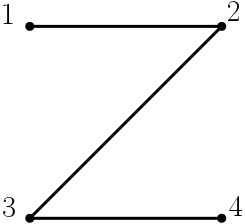
\includegraphics[scale=0.25]{g1}
	\end{subfigure}
\begin{subfigure}[b]{0.16\textwidth}
	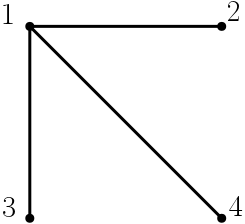
\includegraphics[scale=0.25]{g2}
\end{subfigure}
\begin{subfigure}[b]{0.16\textwidth}
	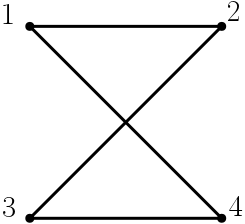
\includegraphics[scale=0.25]{g3}
\end{subfigure}
\begin{subfigure}[b]{0.16\textwidth}
	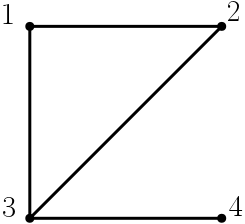
\includegraphics[scale=0.25]{g4}
\end{subfigure}
\begin{subfigure}[b]{0.16\textwidth}
	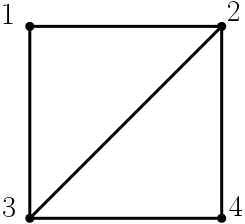
\includegraphics[scale=0.25]{g5}
\end{subfigure}
\begin{subfigure}[b]{0.16\textwidth}
	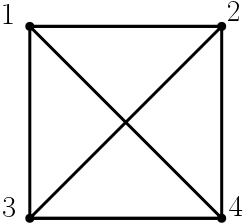
\includegraphics[scale=0.25]{g6}
\end{subfigure}\\
\vspace{0.3cm}
\begin{subfigure}[b]{0.16\textwidth}
	\centering
	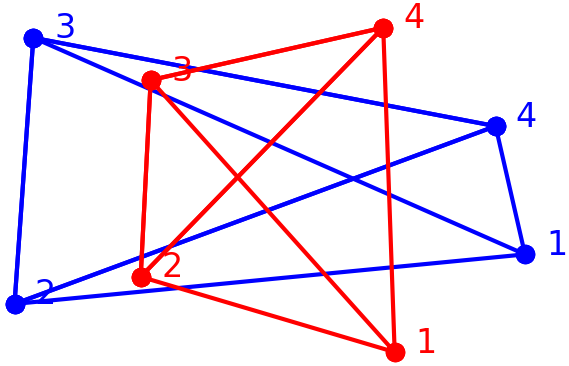
\includegraphics[scale=0.3]{g1_comb}
\end{subfigure}
\begin{subfigure}[b]{0.16\textwidth}
	\centering
	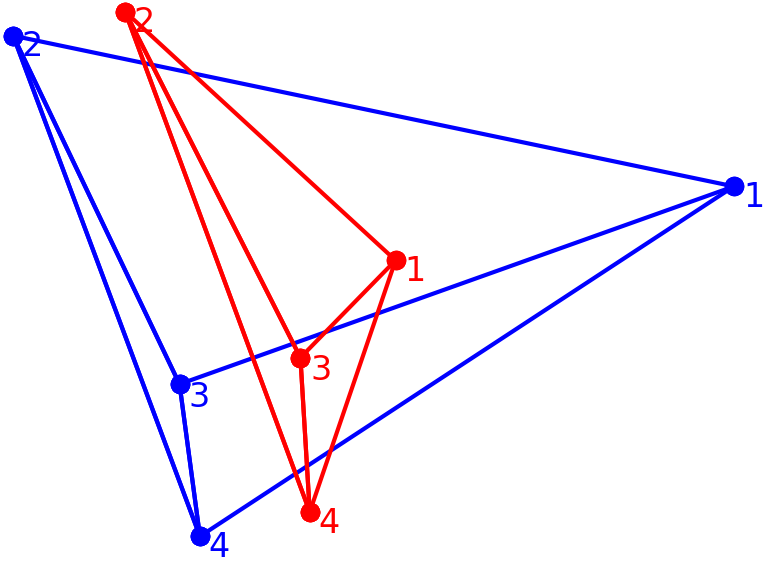
\includegraphics[scale=0.3]{g2_comb}
\end{subfigure}
\begin{subfigure}[b]{0.16\textwidth}
	\centering
	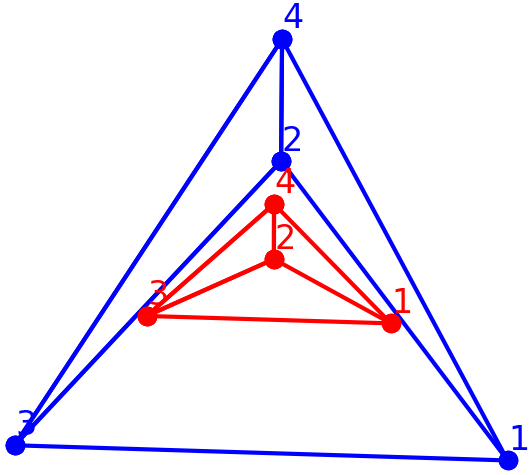
\includegraphics[scale=0.3]{g3_comb}
\end{subfigure}
\begin{subfigure}[b]{0.16\textwidth}
	\centering
	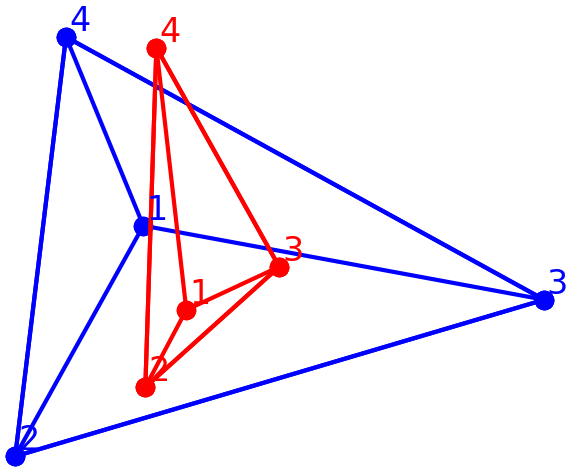
\includegraphics[scale=0.3]{g4_comb}
\end{subfigure}
\begin{subfigure}[b]{0.16\textwidth}
	\centering
	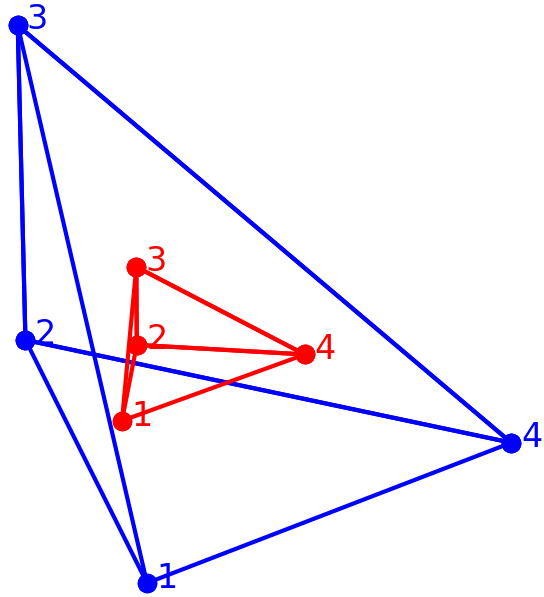
\includegraphics[scale=0.3]{g5_comb}
\end{subfigure}
\begin{subfigure}[b]{0.16\textwidth}
	\centering
	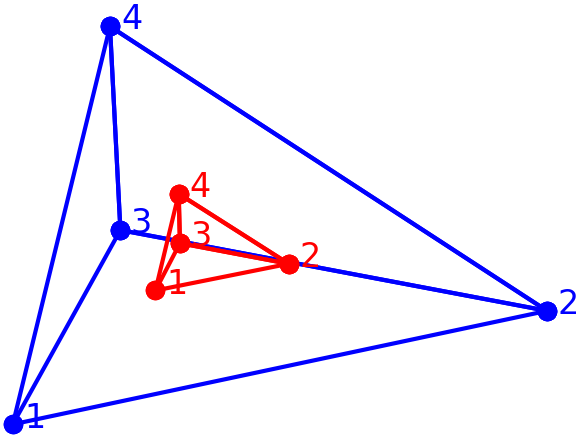
\includegraphics[scale=0.3]{g6_comb}
\end{subfigure}\\
\vspace{0.3cm}
\begin{subfigure}[b]{0.16\textwidth}
	\centering
	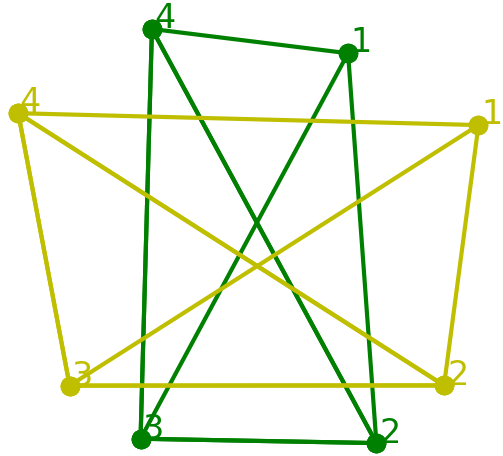
\includegraphics[scale=0.3]{g1_norm}
\end{subfigure}
\begin{subfigure}[b]{0.16\textwidth}
	\centering
	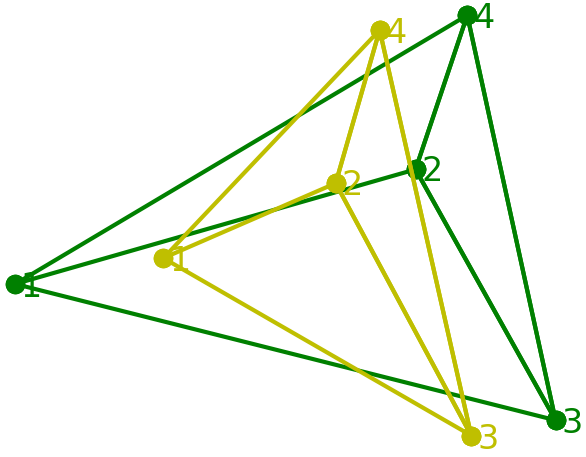
\includegraphics[scale=0.3]{g2_norm}
\end{subfigure}
\begin{subfigure}[b]{0.16\textwidth}
	\centering
	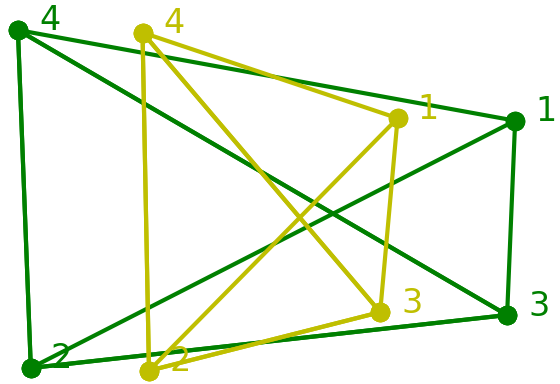
\includegraphics[scale=0.3]{g3_norm}
\end{subfigure}
\begin{subfigure}[b]{0.16\textwidth}
	\centering
	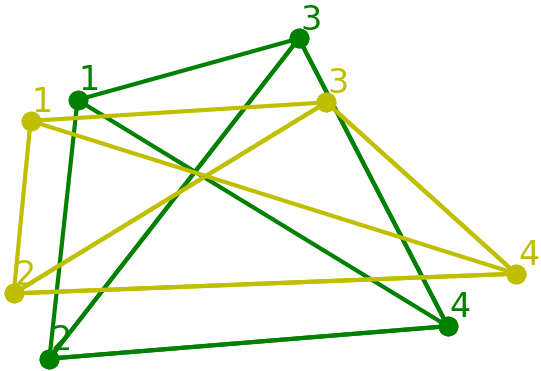
\includegraphics[scale=0.3]{g4_norm}
\end{subfigure}
\begin{subfigure}[b]{0.16\textwidth}
	\centering
	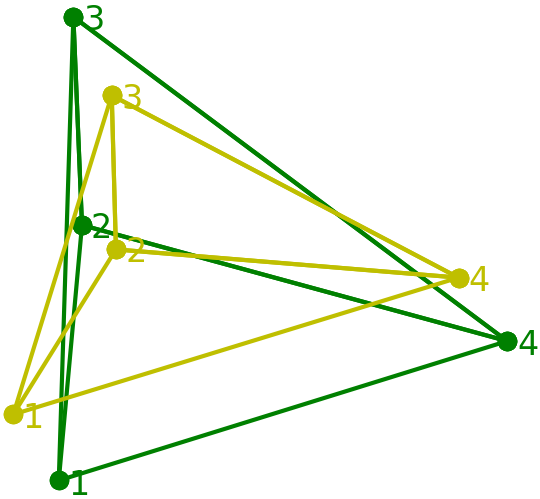
\includegraphics[scale=0.3]{g5_norm}
\end{subfigure}
\begin{subfigure}[b]{0.16\textwidth}
	\centering
	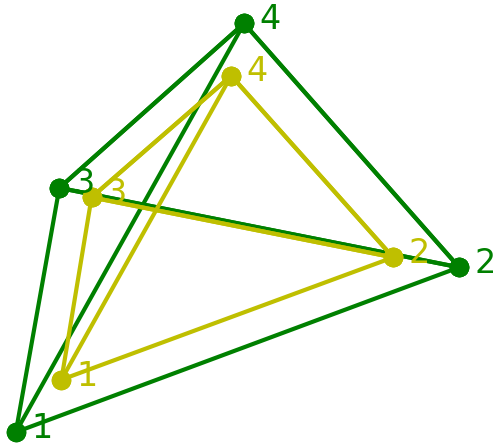
\includegraphics[scale=0.3]{g6_norm}
\end{subfigure}\\

\vspace{0.3cm}
\begin{subfigure}[b]{0.16\textwidth}
	\centering
	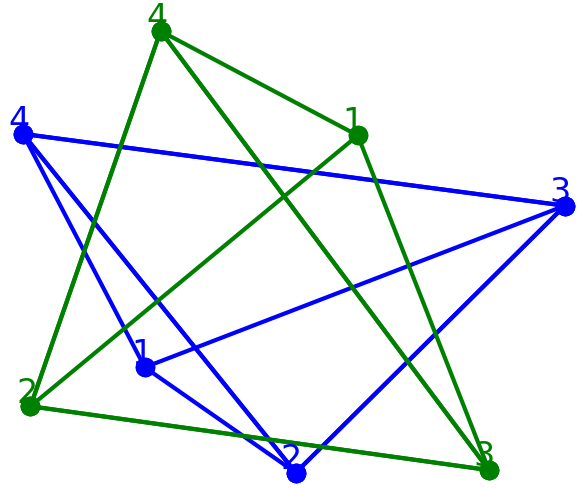
\includegraphics[scale=0.3]{g1_norm_comb}
\end{subfigure}
\begin{subfigure}[b]{0.16\textwidth}
	\centering
	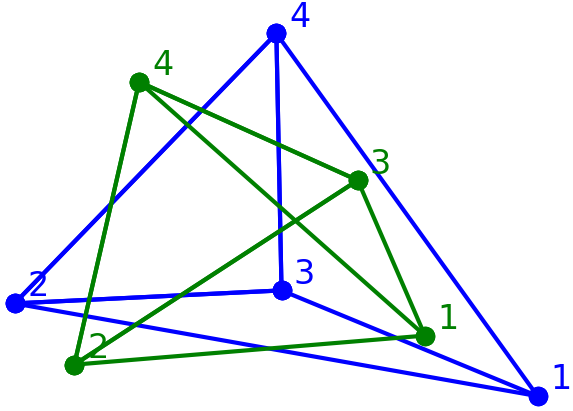
\includegraphics[scale=0.3]{g2_norm_comb}
\end{subfigure}
\begin{subfigure}[b]{0.16\textwidth}
	\centering
	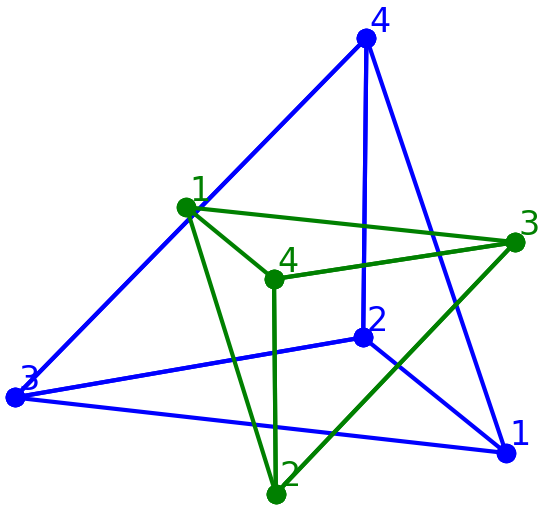
\includegraphics[scale=0.3]{g3_norm_comb}
\end{subfigure}
\begin{subfigure}[b]{0.16\textwidth}
	\centering
	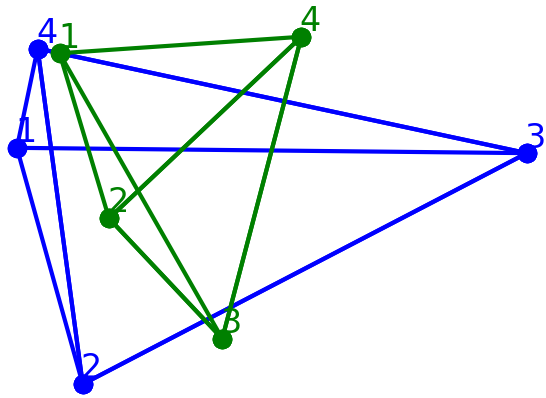
\includegraphics[scale=0.3]{g4_norm_comb}
\end{subfigure}
\begin{subfigure}[b]{0.16\textwidth}
	\centering
	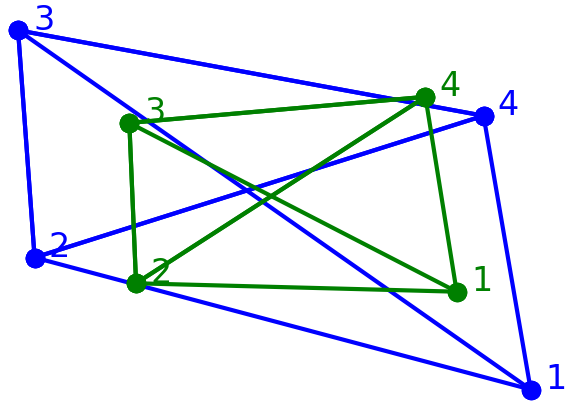
\includegraphics[scale=0.3]{g5_norm_comb}
\end{subfigure}
\begin{subfigure}[b]{0.16\textwidth}
	\centering
	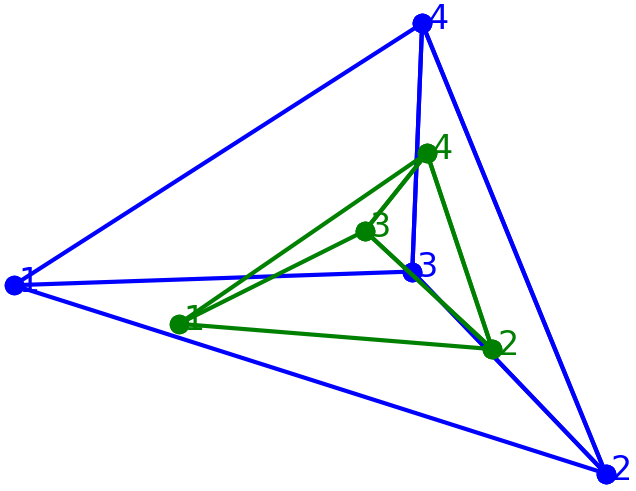
\includegraphics[scale=0.3]{g6_norm_comb}
\end{subfigure}\\
\vspace{0.3cm}
\begin{subfigure}[b]{0.16\textwidth}
	\centering
	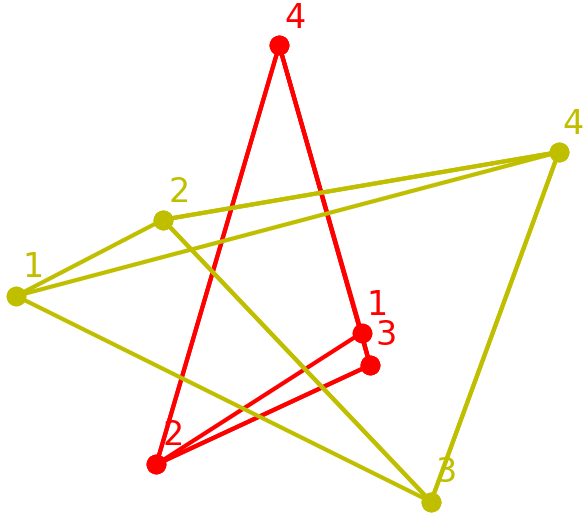
\includegraphics[scale=0.3]{g1_norm_comb_inv}
\end{subfigure}
\begin{subfigure}[b]{0.16\textwidth}
	\centering
	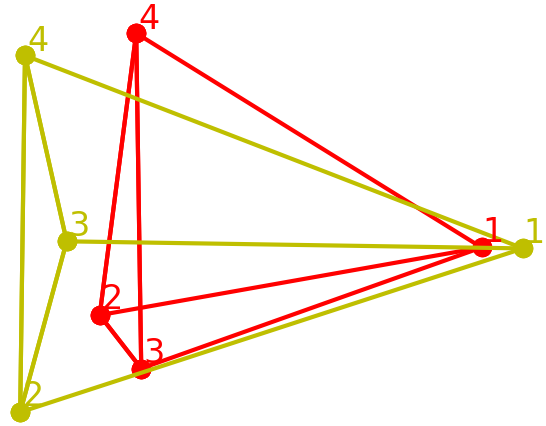
\includegraphics[scale=0.3]{g2_norm_comb_inv}
\end{subfigure}
\begin{subfigure}[b]{0.16\textwidth}
	\centering
	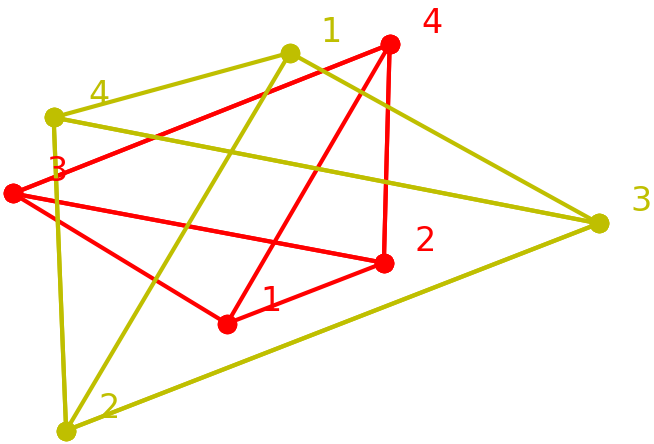
\includegraphics[scale=0.3]{g3_norm_comb_inv}
\end{subfigure}
\begin{subfigure}[b]{0.16\textwidth}
	\centering
	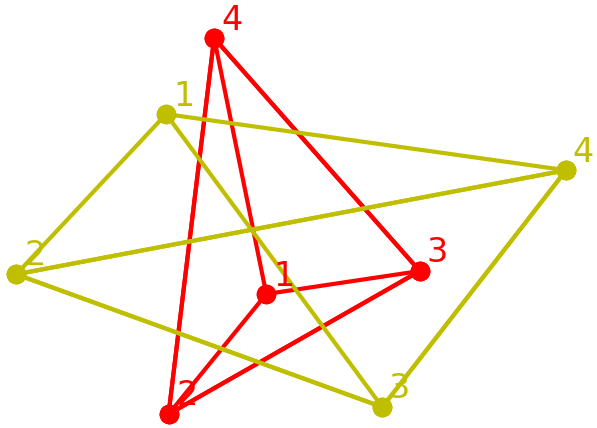
\includegraphics[scale=0.3]{g4_norm_comb_inv}
\end{subfigure}
\begin{subfigure}[b]{0.16\textwidth}
	\centering
	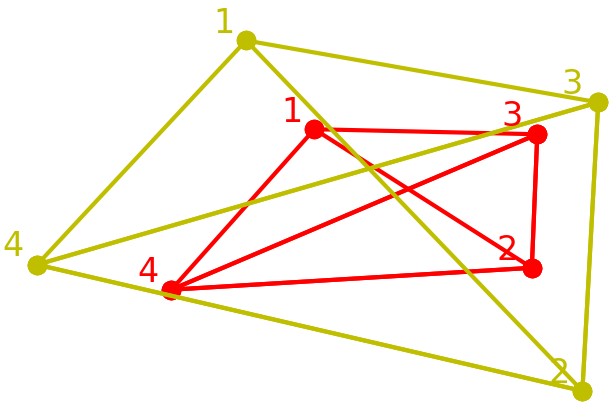
\includegraphics[scale=0.3]{g5_norm_comb_inv}
\end{subfigure}
\begin{subfigure}[b]{0.16\textwidth}
	\centering
	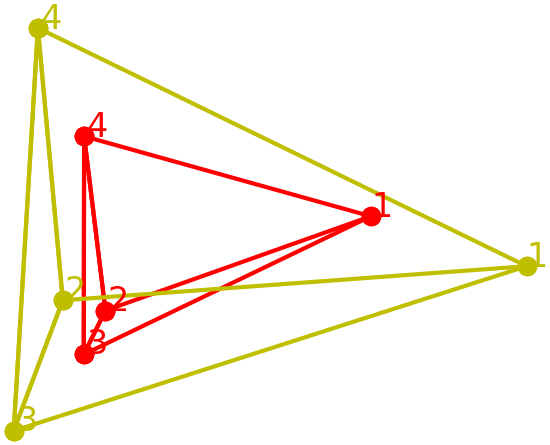
\includegraphics[scale=0.3]{g6_norm_comb_inv}
\end{subfigure}
\caption{The six  unique unweighted  graphs on four vertices, up to isomorphism, and a comparison of all of their simplices. Below each graph in the first row are  its two combinatorial simplices  ($\splx_G$ and $\splx_G^+$), then its two  normalized simplices ($\splxn_G$ and $\splxn_G^+$), then its combinatorial and normalized simplex ($\splx_G$ and $\splxn_G$), followed in  the final  row  by the two inverse simplices ($\splx_G^+$ and $\splxn_G^+$).  The combinatorial simplex and its  inverse are coloured blue and red respectively, and the normalized simplex and its inverse are in green and yellow respectively. The relative size of the the simplices in each subfigure are to scale but the same scale  is not maintained across figures.  }
\label{fig:all_simplices}
\end{figure}











\end{document}
